\documentclass[11pt, a4paper, openany]{book}
\usepackage[a4paper, left=2.5cm, right=2.5cm, top=3cm, bottom=3cm]{geometry}

% Header title
\usepackage{fancyhdr}
\setlength{\headheight}{14pt} % Fix the warning (slightly above suggested)
\pagestyle{fancy}
\fancyhf{} % clear all headers/footers
% \fancyhead[LE,RO]{\thepage}   % Left pages: page number left, right pages: right
% \fancyhead[LO]{\nouppercase{\rightmark}} % Chapter name on odd pages
\fancyhead[LE]{\nouppercase{\leftmark}}  % Section name on even pages
\fancyhead[RO]{\nouppercase{Longitudinal UAD}} % Right pages: short book title
\fancyfoot[C]{\thepage}
\renewcommand{\headrulewidth}{0.4pt}     % Header line thickness
% \renewcommand{\footrulewidth}{0pt}       % No footer line


% \usepackage{arxiv}

\usepackage[utf8]{inputenc} % allow utf-8 input
\usepackage[T1]{fontenc}    % use 8-bit T1 fonts
\usepackage[english]{babel}
\usepackage{csquotes}

% Include cover page
\usepackage{pdfpages}

% Bibliography
\usepackage[
  backend=biber,
  style=numeric,
  % style=alphabetic,
  sorting=none,
  backref=true,
  doi=true,
  url=true,
]{biblatex}
\usepackage{doi}
\AtEveryBibitem{\clearfield{urldate}}
\DeclareSourcemap{  %ignore urldate field to not show (visit on)
  \maps[datatype=bibtex]{
    \map[overwrite=true]{
      \step[fieldset=urldate, null]
    }
  }
}
\addbibresource{references.bib}

% Acronyms
\usepackage[nohyperlinks]{acronym}

%% Math and scientific typesetting
%% The amssymb package provides various useful mathematical symbols
\usepackage{amsfonts}       % blackboard math symbols
\usepackage{nicefrac}       % compact symbols for 1/2, etc.
\usepackage{microtype}      % microtypography
\usepackage[multi-part-units=single]{siunitx}
\sisetup{
  scientific-notation = true,
  retain-unity-mantissa = false,
  exponent-product = \times,
  detect-all=true,
  % detect-inline-weight = math,
  separate-uncertainty,
  output-exponent-marker=\ensuremath{\mathrm{e}}
}

\usepackage{amsmath}
\usepackage{amssymb}
\usepackage{bm}
\usepackage{amssymb}
\usepackage{textcomp}  % for \textuparrow / \textdownarrow

\usepackage{amsmath,amsfonts,bm,amssymb,mathtools,amsthm}
\usepackage{color,xcolor,xspace}
\usepackage{booktabs}
\usepackage{thm-restate}

\newtheorem{theorem}{Theorem}
\newtheorem{definition}{Definition}
\newtheorem{proposition}{Proposition}
\newtheorem{lemma}{Lemma}
\newtheorem{assumption}{Assumption}
\newtheorem{example}{Example}

\newcommand{\figleft}{{\em (Left)}}
\newcommand{\figcenter}{{\em (Center)}}
\newcommand{\figright}{{\em (Right)}}
\newcommand{\figtop}{{\em (Top)}}
\newcommand{\figbottom}{{\em (Bottom)}}
\newcommand{\captiona}{{\em (a)}}
\newcommand{\captionb}{{\em (b)}}
\newcommand{\captionc}{{\em (c)}}
\newcommand{\captiond}{{\em (d)}}
\newcommand{\bb}[1]{{\mathbb{#1}}}
\newcommand{\norm}[1]{{\lVert {#1} \rVert}}
\newcommand{\diff}{\mathrm{d}}
\newcommand{\newterm}[1]{{\bf #1}}


\def\figref#1{figure~\ref{#1}}
\def\Figref#1{Figure~\ref{#1}}
\def\twofigref#1#2{figures \ref{#1} and \ref{#2}}
\def\quadfigref#1#2#3#4{figures \ref{#1}, \ref{#2}, \ref{#3} and \ref{#4}}
\def\secref#1{section~\ref{#1}}
\def\Secref#1{Section~\ref{#1}}
\def\twosecrefs#1#2{sections \ref{#1} and \ref{#2}}
\def\secrefs#1#2#3{sections \ref{#1}, \ref{#2} and \ref{#3}}
\def\eqref#1{Eq.~(\ref{#1})}
\def\Eqref#1{Equation~(\ref{#1})}
\def\plaineqref#1{\ref{#1}}
\def\chapref#1{chapter~\ref{#1}}
\def\Chapref#1{Chapter~\ref{#1}}
\def\rangechapref#1#2{chapters\ref{#1}--\ref{#2}}
\def\algref#1{algorithm~\ref{#1}}
\def\Algref#1{Algorithm~\ref{#1}}
\def\twoalgref#1#2{algorithms \ref{#1} and \ref{#2}}
\def\Twoalgref#1#2{Algorithms \ref{#1} and \ref{#2}}
\def\partref#1{part~\ref{#1}}
\def\Partref#1{Part~\ref{#1}}
\def\twopartref#1#2{parts \ref{#1} and \ref{#2}}

\def\ceil#1{\lceil #1 \rceil}
\def\floor#1{\lfloor #1 \rfloor}
\def\1{\bm{1}}
\newcommand{\train}{\mathcal{D}}
\newcommand{\valid}{\mathcal{D_{\mathrm{valid}}}}
\newcommand{\test}{\mathcal{D_{\mathrm{test}}}}

\def\eps{{\epsilon}}

\def\tq{{\overline{q}}}
\newcommand{\defeq}{\vcentcolon=}
\newcommand{\eqdef}{=\vcentcolon}

\def\reta{{\textnormal{$\eta$}}}
\def\ra{{\textnormal{a}}}
\def\rb{{\textnormal{b}}}
\def\rc{{\textnormal{c}}}
\def\rd{{\textnormal{d}}}
\def\re{{\textnormal{e}}}
\def\rf{{\textnormal{f}}}
\def\rg{{\textnormal{g}}}
\def\rh{{\textnormal{h}}}
\def\ri{{\textnormal{i}}}
\def\rj{{\textnormal{j}}}
\def\rk{{\textnormal{k}}}
\def\rl{{\textnormal{l}}}
\def\rn{{\textnormal{n}}}
\def\ro{{\textnormal{o}}}
\def\rp{{\textnormal{p}}}
\def\rq{{\textnormal{q}}}
\def\rr{{\textnormal{r}}}
\def\rs{{\textnormal{s}}}
\def\rt{{\textnormal{t}}}
\def\ru{{\textnormal{u}}}
\def\rv{{\textnormal{v}}}
\def\rw{{\textnormal{w}}}
\def\rx{{\textnormal{x}}}
\def\ry{{\textnormal{y}}}
\def\rz{{\textnormal{z}}}

\def\rvepsilon{{\mathbf{\epsilon}}}
\def\rvtheta{{\mathbf{\theta}}}
\def\rva{{\mathbf{a}}}
\def\rvb{{\mathbf{b}}}
\def\rvc{{\mathbf{c}}}
\def\rvd{{\mathbf{d}}}
\def\rve{{\mathbf{e}}}
\def\rvf{{\mathbf{f}}}
\def\rvg{{\mathbf{g}}}
\def\rvh{{\mathbf{h}}}
\def\rvu{{\mathbf{i}}}
\def\rvj{{\mathbf{j}}}
\def\rvk{{\mathbf{k}}}
\def\rvl{{\mathbf{l}}}
\def\rvm{{\mathbf{m}}}
\def\rvn{{\mathbf{n}}}
\def\rvo{{\mathbf{o}}}
\def\rvp{{\mathbf{p}}}
\def\rvq{{\mathbf{q}}}
\def\rvr{{\mathbf{r}}}
\def\rvs{{\mathbf{s}}}
\def\rvt{{\mathbf{t}}}
\def\rvu{{\mathbf{u}}}
\def\rvv{{\mathbf{v}}}
\def\rvw{{\mathbf{w}}}
\def\rvx{{\mathbf{x}}}
\def\rvy{{\mathbf{y}}}
\def\rvz{{\mathbf{z}}}

\def\erva{{\textnormal{a}}}
\def\ervb{{\textnormal{b}}}
\def\ervc{{\textnormal{c}}}
\def\ervd{{\textnormal{d}}}
\def\erve{{\textnormal{e}}}
\def\ervf{{\textnormal{f}}}
\def\ervg{{\textnormal{g}}}
\def\ervh{{\textnormal{h}}}
\def\ervi{{\textnormal{i}}}
\def\ervj{{\textnormal{j}}}
\def\ervk{{\textnormal{k}}}
\def\ervl{{\textnormal{l}}}
\def\ervm{{\textnormal{m}}}
\def\ervn{{\textnormal{n}}}
\def\ervo{{\textnormal{o}}}
\def\ervp{{\textnormal{p}}}
\def\ervq{{\textnormal{q}}}
\def\ervr{{\textnormal{r}}}
\def\ervs{{\textnormal{s}}}
\def\ervt{{\textnormal{t}}}
\def\ervu{{\textnormal{u}}}
\def\ervv{{\textnormal{v}}}
\def\ervw{{\textnormal{w}}}
\def\ervx{{\textnormal{x}}}
\def\ervy{{\textnormal{y}}}
\def\ervz{{\textnormal{z}}}

\def\rmA{{\mathbf{A}}}
\def\rmB{{\mathbf{B}}}
\def\rmC{{\mathbf{C}}}
\def\rmD{{\mathbf{D}}}
\def\rmE{{\mathbf{E}}}
\def\rmF{{\mathbf{F}}}
\def\rmG{{\mathbf{G}}}
\def\rmH{{\mathbf{H}}}
\def\rmI{{\mathbf{I}}}
\def\rmJ{{\mathbf{J}}}
\def\rmK{{\mathbf{K}}}
\def\rmL{{\mathbf{L}}}
\def\rmM{{\mathbf{M}}}
\def\rmN{{\mathbf{N}}}
\def\rmO{{\mathbf{O}}}
\def\rmP{{\mathbf{P}}}
\def\rmQ{{\mathbf{Q}}}
\def\rmR{{\mathbf{R}}}
\def\rmS{{\mathbf{S}}}
\def\rmT{{\mathbf{T}}}
\def\rmU{{\mathbf{U}}}
\def\rmV{{\mathbf{V}}}
\def\rmW{{\mathbf{W}}}
\def\rmX{{\mathbf{X}}}
\def\rmY{{\mathbf{Y}}}
\def\rmZ{{\mathbf{Z}}}

\def\ermA{{\textnormal{A}}}
\def\ermB{{\textnormal{B}}}
\def\ermC{{\textnormal{C}}}
\def\ermD{{\textnormal{D}}}
\def\ermE{{\textnormal{E}}}
\def\ermF{{\textnormal{F}}}
\def\ermG{{\textnormal{G}}}
\def\ermH{{\textnormal{H}}}
\def\ermI{{\textnormal{I}}}
\def\ermJ{{\textnormal{J}}}
\def\ermK{{\textnormal{K}}}
\def\ermL{{\textnormal{L}}}
\def\ermM{{\textnormal{M}}}
\def\ermN{{\textnormal{N}}}
\def\ermO{{\textnormal{O}}}
\def\ermP{{\textnormal{P}}}
\def\ermQ{{\textnormal{Q}}}
\def\ermR{{\textnormal{R}}}
\def\ermS{{\textnormal{S}}}
\def\ermT{{\textnormal{T}}}
\def\ermU{{\textnormal{U}}}
\def\ermV{{\textnormal{V}}}
\def\ermW{{\textnormal{W}}}
\def\ermX{{\textnormal{X}}}
\def\ermY{{\textnormal{Y}}}
\def\ermZ{{\textnormal{Z}}}

\def\vzero{{\bm{0}}}
\def\vone{{\bm{1}}}
\def\vmu{{\bm{\mu}}}
\def\vtheta{{\bm{\theta}}}
\def\vpsi{{\bm{\psi}}}
\def\va{{\bm{a}}}
\def\vb{{\bm{b}}}
\def\vc{{\bm{c}}}
\def\vd{{\bm{d}}}
\def\ve{{\bm{e}}}
\def\vf{{\bm{f}}}
\def\vg{{\bm{g}}}
\def\vh{{\bm{h}}}
\def\vi{{\bm{i}}}
\def\vj{{\bm{j}}}
\def\vk{{\bm{k}}}
\def\vl{{\bm{l}}}
\def\vm{{\bm{m}}}
\def\vn{{\bm{n}}}
\def\vo{{\bm{o}}}
\def\vp{{\bm{p}}}
\def\vq{{\bm{q}}}
\def\vr{{\bm{r}}}
\def\vs{{\bm{s}}}
\def\vt{{\bm{t}}}
\def\vu{{\bm{u}}}
\def\vv{{\bm{v}}}
\def\vw{{\bm{w}}}
\def\vx{{\bm{x}}}
\def\vy{{\bm{y}}}
\def\vz{{\bm{z}}}
\def\vpi{{\bm{\pi}}}
\def\vomega{{\bm{\omega}}}
\def\vlambda{{\bm{\lambda}}}
\def\vtheta{{\bm{\theta}}}
\def\vphi{{\bm{\phi}}}
\def\vmu{{\bm{\mu}}}
\def\Hw{{H_\vomega(\vx)}}
\def\Et{{E_\vtheta(\vx)}}
\def\HE{{\Hw + \Et}}
\newcommand{\at}[2][]{#1|_{#2}}
\def\otheta{{\vtheta^*}}
\def\oomega{{\vomega^*}}
\def\ophi{{\vphi^*}}
\def\vJ{{\bm{J}}}
\def\vK{{\bm{K}}}
\def\vP{{\bm{P}}}
\def\vQ{{\bm{Q}}}
\def\vS{{\bm{S}}}
\def\vU{{\bm{U}}}
\def\vW{{\bm{W}}}
\def\vI{{\bm{I}}}

\def\evalpha{{\alpha}}
\def\evbeta{{\beta}}
\def\evepsilon{{\epsilon}}
\def\evlambda{{\lambda}}
\def\evomega{{\omega}}
\def\evmu{{\mu}}
\def\evpsi{{\psi}}
\def\evsigma{{\sigma}}
\def\evtheta{{\theta}}
\def\eva{{a}}
\def\evb{{b}}
\def\evc{{c}}
\def\evd{{d}}
\def\eve{{e}}
\def\evf{{f}}
\def\evg{{g}}
\def\evh{{h}}
\def\evi{{i}}
\def\evj{{j}}
\def\evk{{k}}
\def\evl{{l}}
\def\evm{{m}}
\def\evn{{n}}
\def\evo{{o}}
\def\evp{{p}}
\def\evq{{q}}
\def\evr{{r}}
\def\evs{{s}}
\def\evt{{t}}
\def\evu{{u}}
\def\evv{{v}}
\def\evw{{w}}
\def\evx{{x}}
\def\evy{{y}}
\def\evz{{z}}

\def\mA{{\bm{A}}}
\def\mB{{\bm{B}}}
\def\mC{{\bm{C}}}
\def\mD{{\bm{D}}}
\def\mE{{\bm{E}}}
\def\mF{{\bm{F}}}
\def\mG{{\bm{G}}}
\def\mH{{\bm{H}}}
\def\mI{{\bm{I}}}
\def\mJ{{\bm{J}}}
\def\mK{{\bm{K}}}
\def\mL{{\bm{L}}}
\def\mM{{\bm{M}}}
\def\mN{{\bm{N}}}
\def\mO{{\bm{O}}}
\def\mP{{\bm{P}}}
\def\mQ{{\bm{Q}}}
\def\mR{{\bm{R}}}
\def\mS{{\bm{S}}}
\def\mT{{\bm{T}}}
\def\mU{{\bm{U}}}
\def\mV{{\bm{V}}}
\def\mW{{\bm{W}}}
\def\mX{{\bm{X}}}
\def\mY{{\bm{Y}}}
\def\mZ{{\bm{Z}}}
\def\mBeta{{\bm{\beta}}}
\def\mPhi{{\bm{\Phi}}}
\def\mLambda{{\bm{\Lambda}}}
\def\mSigma{{\bm{\Sigma}}}

\DeclareMathAlphabet{\mathsfit}{\encodingdefault}{\sfdefault}{m}{sl}
\SetMathAlphabet{\mathsfit}{bold}{\encodingdefault}{\sfdefault}{bx}{n}
\newcommand{\tens}[1]{\bm{\mathsfit{#1}}}
\def\tA{{\tens{A}}}
\def\tB{{\tens{B}}}
\def\tC{{\tens{C}}}
\def\tD{{\tens{D}}}
\def\tE{{\tens{E}}}
\def\tF{{\tens{F}}}
\def\tG{{\tens{G}}}
\def\tH{{\tens{H}}}
\def\tI{{\tens{I}}}
\def\tJ{{\tens{J}}}
\def\tK{{\tens{K}}}
\def\tL{{\tens{L}}}
\def\tM{{\tens{M}}}
\def\tN{{\tens{N}}}
\def\tO{{\tens{O}}}
\def\tP{{\tens{P}}}
\def\tQ{{\tens{Q}}}
\def\tR{{\tens{R}}}
\def\tS{{\tens{S}}}
\def\tT{{\tens{T}}}
\def\tU{{\tens{U}}}
\def\tV{{\tens{V}}}
\def\tW{{\tens{W}}}
\def\tX{{\tens{X}}}
\def\tY{{\tens{Y}}}
\def\tZ{{\tens{Z}}}


\def\gA{{\mathcal{A}}}
\def\gB{{\mathcal{B}}}
\def\gC{{\mathcal{C}}}
\def\gD{{\mathcal{D}}}
\def\gE{{\mathcal{E}}}
\def\gF{{\mathcal{F}}}
\def\gG{{\mathcal{G}}}
\def\gH{{\mathcal{H}}}
\def\gI{{\mathcal{I}}}
\def\gJ{{\mathcal{J}}}
\def\gK{{\mathcal{K}}}
\def\gL{{\mathcal{L}}}
\def\gM{{\mathcal{M}}}
\def\gN{{\mathcal{N}}}
\def\gO{{\mathcal{O}}}
\def\gP{{\mathcal{P}}}
\def\gQ{{\mathcal{Q}}}
\def\gR{{\mathcal{R}}}
\def\gS{{\mathcal{S}}}
\def\gT{{\mathcal{T}}}
\def\gU{{\mathcal{U}}}
\def\gV{{\mathcal{V}}}
\def\gW{{\mathcal{W}}}
\def\gX{{\mathcal{X}}}
\def\gY{{\mathcal{Y}}}
\def\gZ{{\mathcal{Z}}}

\def\sA{{\mathbb{A}}}
\def\sB{{\mathbb{B}}}
\def\sC{{\mathbb{C}}}
\def\sD{{\mathbb{D}}}
\def\sF{{\mathbb{F}}}
\def\sG{{\mathbb{G}}}
\def\sH{{\mathbb{H}}}
\def\sI{{\mathbb{I}}}
\def\sJ{{\mathbb{J}}}
\def\sK{{\mathbb{K}}}
\def\sL{{\mathbb{L}}}
\def\sM{{\mathbb{M}}}
\def\sN{{\mathbb{N}}}
\def\sO{{\mathbb{O}}}
\def\sP{{\mathbb{P}}}
\def\sQ{{\mathbb{Q}}}
\def\sR{{\mathbb{R}}}
\def\sS{{\mathbb{S}}}
\def\sT{{\mathbb{T}}}
\def\sU{{\mathbb{U}}}
\def\sV{{\mathbb{V}}}
\def\sW{{\mathbb{W}}}
\def\sX{{\mathbb{X}}}
\def\sY{{\mathbb{Y}}}
\def\sZ{{\mathbb{Z}}}

\def\emLambda{{\Lambda}}
\def\emA{{A}}
\def\emB{{B}}
\def\emC{{C}}
\def\emD{{D}}
\def\emE{{E}}
\def\emF{{F}}
\def\emG{{G}}
\def\emH{{H}}
\def\emI{{I}}
\def\emJ{{J}}
\def\emK{{K}}
\def\emL{{L}}
\def\emM{{M}}
\def\emN{{N}}
\def\emO{{O}}
\def\emP{{P}}
\def\emQ{{Q}}
\def\emR{{R}}
\def\emS{{S}}
\def\emT{{T}}
\def\emU{{U}}
\def\emV{{V}}
\def\emW{{W}}
\def\emX{{X}}
\def\emY{{Y}}
\def\emZ{{Z}}
\def\emSigma{{\Sigma}}

\newcommand{\etens}[1]{\mathsfit{#1}}
\def\etLambda{{\etens{\Lambda}}}
\def\etA{{\etens{A}}}
\def\etB{{\etens{B}}}
\def\etC{{\etens{C}}}
\def\etD{{\etens{D}}}
\def\etE{{\etens{E}}}
\def\etF{{\etens{F}}}
\def\etG{{\etens{G}}}
\def\etH{{\etens{H}}}
\def\etI{{\etens{I}}}
\def\etJ{{\etens{J}}}
\def\etK{{\etens{K}}}
\def\etL{{\etens{L}}}
\def\etM{{\etens{M}}}
\def\etN{{\etens{N}}}
\def\etO{{\etens{O}}}
\def\etP{{\etens{P}}}
\def\etQ{{\etens{Q}}}
\def\etR{{\etens{R}}}
\def\etS{{\etens{S}}}
\def\etT{{\etens{T}}}
\def\etU{{\etens{U}}}
\def\etV{{\etens{V}}}
\def\etW{{\etens{W}}}
\def\etX{{\etens{X}}}
\def\etY{{\etens{Y}}}
\def\etZ{{\etens{Z}}}

\newcommand{\pdata}{p_{\rm{data}}}
\newcommand{\ptrain}{\hat{p}_{\rm{data}}}
\newcommand{\Ptrain}{\hat{P}_{\rm{data}}}
\newcommand{\pmodel}{p_{\rm{model}}}
\newcommand{\Pmodel}{P_{\rm{model}}}
\newcommand{\ptildemodel}{\tilde{p}_{\rm{model}}}
\newcommand{\pencode}{p_{\rm{encoder}}}
\newcommand{\pdecode}{p_{\rm{decoder}}}
\newcommand{\precons}{p_{\rm{reconstruct}}}

\newcommand{\laplace}{\mathrm{Laplace}} %

\newcommand{\E}{\mathbb{E}}
\newcommand{\Ls}{\mathcal{L}}
\newcommand{\R}{\mathbb{R}}
\newcommand{\emp}{\tilde{p}}
\newcommand{\lr}{\alpha}
\newcommand{\reg}{\lambda}
\newcommand{\rect}{\mathrm{rectifier}}
\newcommand{\softmax}{\mathrm{softmax}}
\newcommand{\sigmoid}{\sigma}
\newcommand{\softplus}{\zeta}
\newcommand{\KL}{D_{\mathrm{KL}}}
\newcommand{\DF}{D_f}
\newcommand{\Var}{\mathrm{Var}}
\newcommand{\standarderror}{\mathrm{SE}}
\newcommand{\Cov}{\mathrm{Cov}}
\newcommand{\normlzero}{L^0}
\newcommand{\normlone}{L^1}
\newcommand{\normltwo}{L^2}
\newcommand{\normlp}{L^p}
\newcommand{\normmax}{L^\infty}

\newcommand{\parents}{Pa} %

\DeclareMathOperator*{\argmax}{arg\,max}
\DeclareMathOperator*{\argmin}{arg\,min}

\DeclareMathOperator{\sign}{sign}
\DeclareMathOperator{\Tr}{Tr}
\let\ab\allowbreak
\newcommand\numberthis{\addtocounter{equation}{1}\tag{\theequation}}

\newcommand{\js}[1]{{\color{teal} [JS: #1]}}
\newcommand{\se}[1]{{\color{magenta} [SE: #1]}}
\newcommand{\kk}[1]{{\color{blue} [KK: #1]}}
\renewcommand{\emptyset}{\varnothing}
\newcommand{\dop}{\mathrm{do}}
\newcommand{\supp}{\mathrm{supp}}

%% Figures and Tables format and placement
\usepackage{float}
\usepackage{placeins}
\usepackage{booktabs}       % professional-quality tables
\usepackage{subcaption}
\usepackage{framed,multirow}
\usepackage{graphicx}
\usepackage{xcolor}
\usepackage{adjustbox}

% MiniToC for ToC at the beginning of each chapter
\usepackage{minitoc}
\dominitoc  % activate minitocs

% Support for easy cross-referencing
\usepackage[capitalize]{cleveref}
\crefname{section}{Sec.}{Secs.}
\Crefname{section}{Section}{Sections}
\Crefname{table}{Table}{Tables}
\crefname{table}{Tab.}{Tabs.}
\crefname{equation}{E.q}{E.qs}
\Crefname{equation}{E.q}{E.qs}
% \crefname{app}{Appendix}{Appendices}
% \Crefname{app}{Appendix}{Appendices}

\newcommand{\cmark}{\ding{51}}%
\newcommand{\xmark}{\ding{55}}
\newcommand{\subsubsubsection}[1]{%
  \vspace{1em}%
  \noindent\textbf{#1}\quad
}

%% Hyperref
\usepackage{url}            % simple URL typesetting
\usepackage{xurl}
\usepackage{hyperref}
\hypersetup{
  breaklinks=true,
  colorlinks=true,
  linkcolor=blue,
  citecolor=blue,
  urlcolor=magenta
}

\title{Longitudinal Unsupervised Anomaly Detection (UAD) with diffusion models}

%\date{September 9, 1985}  % Here you can change the date presented in the paper title
%\date{}           % Or removing it

\author{ Ba-Khuong Dang\\
  ENSAI\\
INRIA Grenoble }

% Uncomment to remove the date
\date{}

% Uncomment to override  the `A preprint' in the header
% \renewcommand{\headeright}{Preprint}
% \renewcommand{\undertitle}{}
% \renewcommand{\shorttitle}{Behrendt et al. \textit{Conditioned Diffusion Models for UAD in Brain MRIs}}

%%% Add PDF metadata to help others organize their library
%%% Once the PDF is generated, you can check the metadata with
%%% $ pdfinfo template.pdf
% \hypersetup{
% pdftitle={A template for the arxiv style},
% pdfsubject={q-bio.NC, q-bio.QM},
% pdfauthor={David S.~Hippocampus, Elias D.~Striatum},
% pdfkeywords={First keyword, Second keyword, More},
% }

\begin{document}

% Cover page
% \pagestyle{empty}
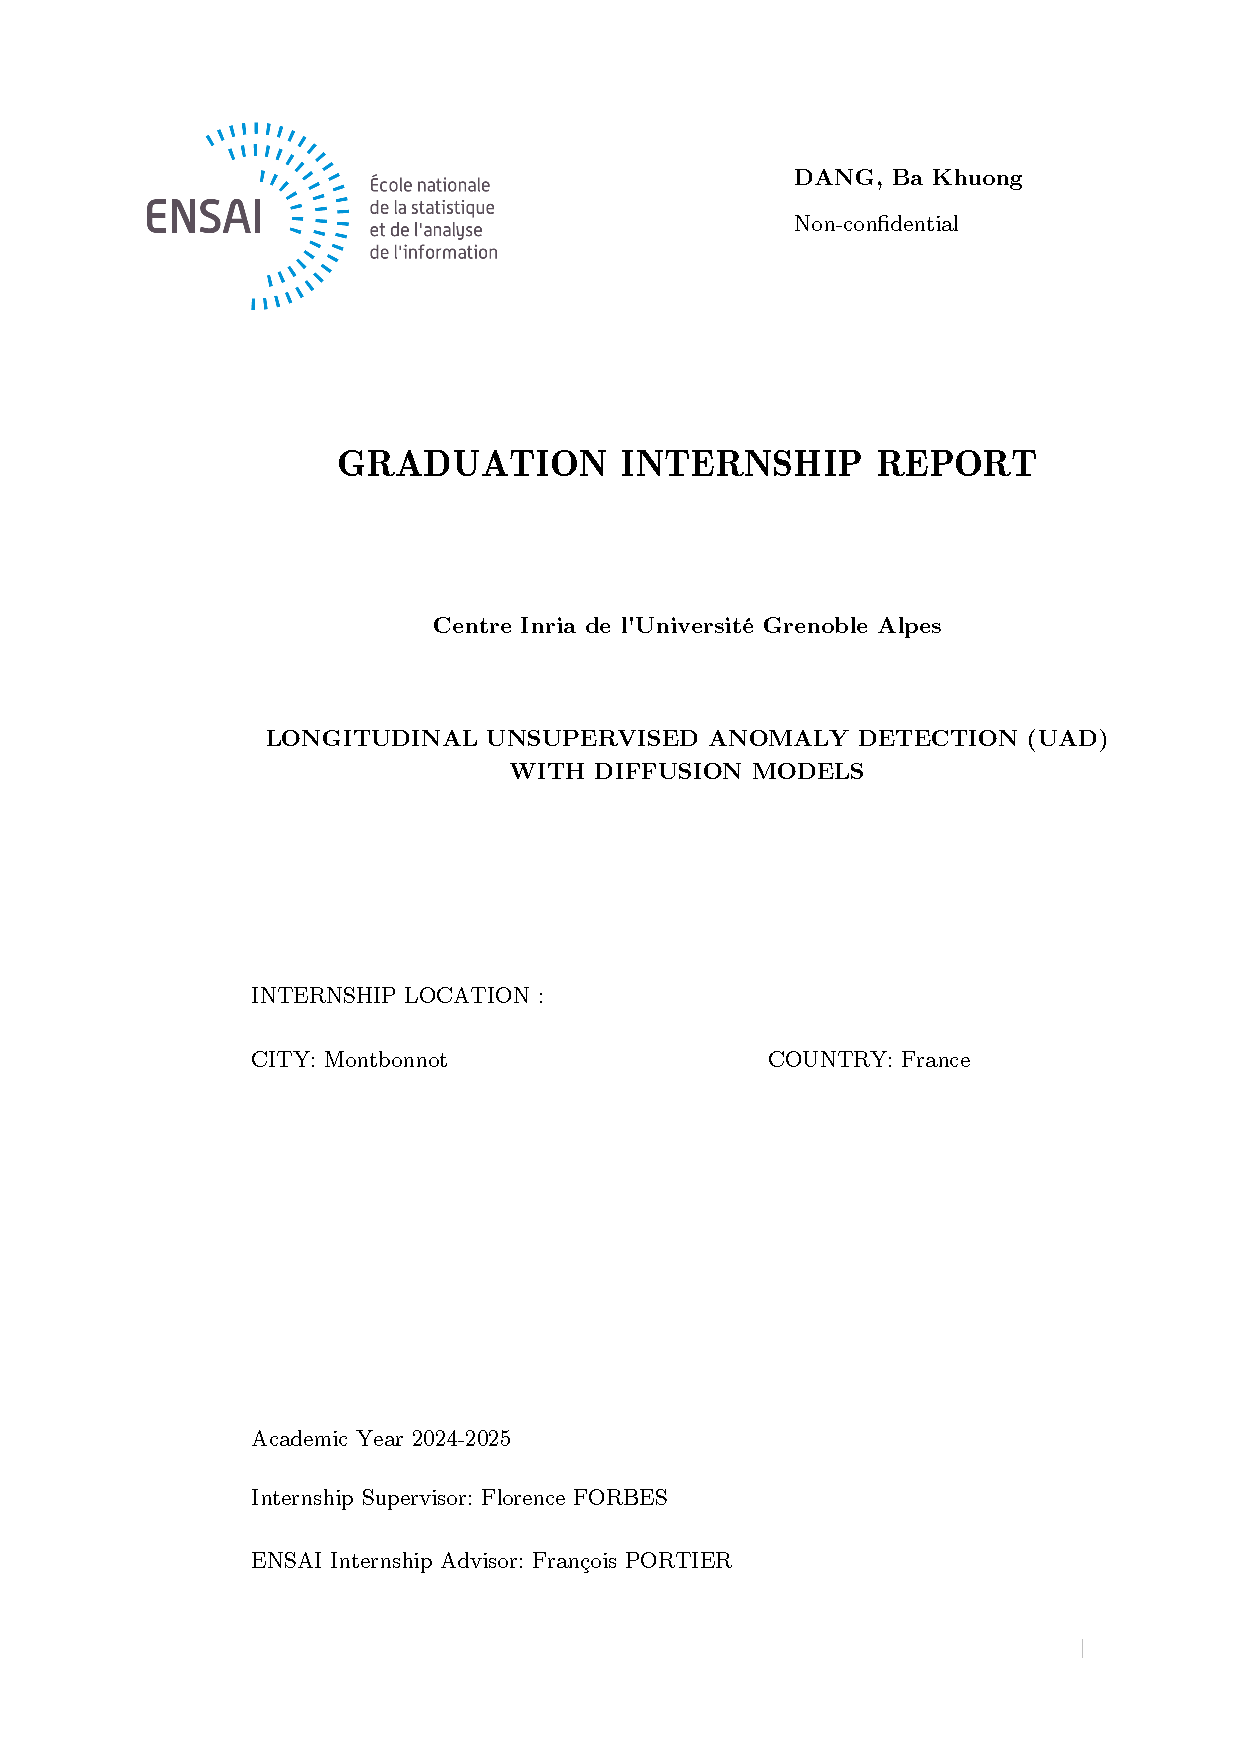
\includepdf[pages={1}]{cover.pdf}
\setcounter{page}{1}

% Title page
\frontmatter
\maketitle

% \begin{abstract}
% The application of supervised models to clinical screening tasks is challenging due to the need for annotated data for each considered pathology. Unsupervised Anomaly Detection (UAD) is an alternative approach that aims to identify any anomaly as an outlier from a healthy training distribution. A prevalent strategy for UAD in brain MRI involves using generative models to learn the reconstruction of healthy brain anatomy for a given input image. As these models should fail to reconstruct unhealthy structures, the reconstruction errors indicate anomalies. However, a significant challenge is to balance the accurate reconstruction of healthy anatomy and the undesired replication of abnormal structures. While diffusion models have shown promising results with detailed and accurate reconstructions, they face challenges in preserving intensity characteristics, resulting in false positives.
% \end{abstract}


% Acknowledgement
\chapter*{Acknowledgements}
I would like to express my sincere gratitude for the opportunity to work on this
project with Statify team at Inria Grenoble. Special thanks to my internship supervisors Dr. Florence Forbes
for her constructive feedback and advice throughout the entire project. Her expertise and insightful guidance were instrumental in addressing some of our key challenges. Additionally, I extend my appreciation to my ENSAI professors, specially my internship advisor professor Francois Portier, for their amazing academic guidance.
\clearpage

% ToC
\tableofcontents

% Define acronym
\chapter*{List of Acronyms}
\begin{acronym}[AUPRC]
  \acro{AD}{Anomaly Detection}
  \acro{AUROC}{Area Under the Receiver Operating Characteristic curve}
  \acro{AUPRC}{Area Under the Precision-Recall curve}
  \acro{DDIMs}{Denoising implicit models}
  \acro{DDPMs}{Denoising Probabilistic Diffusion Models}
  \acro{DMs}{Diffusion Models}
  \acro{FA}{Feature Attention}
  \acro{FAM}{Feature Attention Module}
  \acro{FN}{False Negative}
  \acro{FP}{False Positive}
  \acro{GAN}{Generative Adversarial Networks}
  \acro{GMs}{Generative Models}
  \acro{LAF}{Longitudinal Attention Fusion}
  \acro{LAFM}{Longitudinal Attention Fusion Module}
  \acro{SDM}{Spatial Diffusion Model}
  \acro{TDM}{Temporal Diffusion Model}
  \acro{TN}{True Negative}
  \acro{TP}{True Positive}
  \acro{UAD}{Unsupervised Anomaly Detection}
  \acro{VAE}{Variational Autoencoders}
\end{acronym}

% List of Notations / Symbols
\chapter*{List of Notations / Symbols}
% \resizebox{\textwidth}{!}{%
\begin{tabular}{l@{\hspace{1.5cm}}p{13cm}}
  % \hline
  % \textbf{Symbol} & \textbf{Description} \\
  % \hline
  $\mathbf{X}^i_{1 \leq i \leq N}$ & Set of observed images of patient $i$ through time \\
  $N$ & Number of patients \\
  $\rvx^i_l$ & Observation of patient $i$ at time point $l$. We often omit superscript $i$ and subscript $l$ for brevity. \\
  $l \in [1 \dots L]$ & Longitudinal time point (time indexed) \\
  $\rvx$      & Original image (potential anomalous) $\in \mathbb{R}^{h \times w}$ \\
  $\hat\rvx$      & Reconstructed image (can be psuedo-healthy) $\in \mathbb{R}^{h \times w}$\\
  $D_p$      & Pixel anomaly score map / pixel distance $\in \mathbb{R}^{h \times w}$\\
  $D_f$ & Feature distance $\in \mathbb{R}^{h \times w}$\\
  $q(\rvx)$ & True probability distribution of $\rvx$ that we want to learn and sample from. \\
  $p_{\theta}(\rvx)$ & Estimated distribution of $\rvx$ from diffusion model. \\
  $\epsilon_{\theta}$ & Output of diffusion model, with parameter $\epsilon$. \\
  $\mu_{\theta}(t), \Sigma_{\theta}(t)$ & Mean and variance of predicted posterior of diffusion model. \\
  $\text{Enc}_{\phi}$ & Semantic encoder with parameter $\phi$ \\
  $\rvy$ ($\rvy_{\text{sem}}$) & Semantic representation of $\rvx \in \mathbb{R}^d$ \\
  $\beta_t$ & Noise schedule of diffusion model. \\
  $t \in [1 \dots T]$ & Time step of diffusion model \\
  $\Phi$ ($\text{FE}_{\Phi}$) & Feaure extractor network from FAM, with parameter $\Phi$ \\
  $\lambda_{DL}$ & Hyperparameter of Feature Extract network controls the strength of distillation losses \\
  $v$ & Hyperparameter of FAM that controls the importance of pixel error \\
  $\rvs$, $D_{\text{anomaly}}$ & Anomaly score map $\in \mathbb{R}^{h \times w}$ from FAM \\
  $\mathbf{S}_i$ & Set of anomaly score map for $L$ time point for 1 patient $i$ \\
  $\rvs_{\text{ref}}$ & Reference anomaly score map $\in \mathbb{R}^{(L-1) \times h \times w}$ for 1 target anomaly score map (LAFM module)\\
  $\rvs_{\text{temp}}$ & Updated anomaly score map from LAFM after temporal smoothing operator \\
  $\mathbf{S}_{\text{temp}}$ & Set of updated anomaly score map from LAFM $\in \mathbb{R}^{L \times h \times w}$ \\
  $\beta$, $\gamma$ & Hyperparameters of LAFM that control the correction of false positive and false negative \\
  $k_{mf}$ & Kernal size of median filter of LAFM \\
  $\mathbf{X}_i^{\mathcal{O}}$ & Set of observed data for patient $i$. We often omit subscript $i$ for brevity \\
  $\mathbf{X}_i^{\mathcal{M}}$ & Set of missing data for patient $i$. We often omit subscript $i$ for brevity \\
  $\text{Enc}_{\omega}$ & Semantic encoder of TDM (RRDB net) \\
  $\mathbf{Z}$ & List of semantic representation from semantic encoder RRDB in TDM \\
  $\mathbf{z}_{\text{sem}, i} \in \mathbf{Z}$ & Semantic representation from block $i$ of RRDB $\in \mathbb{R}^{h \times w}$ \\
  % \hline
\end{tabular}

% List of figures
\listoffigures

% List of Tables
\listoftables

% Main sections
% \clearpage
% \pagestyle{plain}
% \setcounter{page}{1}
\mainmatter
\chapter{Introduction}
\label{chap:introduction}
\minitoc

\ac{AD} and anomaly localization in medical images refer to the process of identifying abnormal areas or regions within images of various modalities, one of which is Magnetic Resonance Imaging (MRI) scans. Fully supervised deep learning approaches have demonstrated robust performance in assisting radiologists with MRI interpretation and automating tasks such as anomaly segmentation. For example, UNet-based algorithms have significantly contributed to advancements in automatic lesion segmentation. However, these methods require large datasets with image-level labels and pixel-level annotations for training, which are typically expensive and time consuming to obtain. Furthermore, the subtle nature of certain anomalies makes them difficult to detect, even for human experts. Consequently, rare and subtle anomalies may be underrepresented or entirely absent from training datasets, reducing the robustness of supervised approaches. An alternative is \ac{UAD}, which relies solely on healthy data rather than annotated pathological examples. The objective is to learn the underlying distribution of healthy brain MRI scans, and then to detect anomalies as deviations from this learned distribution. In recent study, \cite{lagogiannisUADStudyOfSOTA} categorize UAD methods into four groups: image reconstruction-based, feature-modeling, attention-based and self-supervised anomaly detection methods. In this project, we will focus on the reconstruction-based method, in particular using diffusion models. Additionally, longitudinal data in MRI scans provide repeated measurements of the same subject over time, offering valuable insights into disease progression and temporal patterns. In the context of \ac{UAD}, most \ac{DMs} treat each image independently (spatial dimension), without considering longitudinal dependencies (temporal dimension). Our goal is to investigate the viability of leveraging additional information provided by longitudinal data. Our source code is available at \url{https://github.com/khuongdb/spatio-temporal-DM}\footnote{At the time of writing, we are still developing and expanding the project. The source code is not yet fully refined.}.  

\section{Reconstruction-based UAE with diffusion models}
\label{sec:introduction-sdm}

\begin{figure}
    \centering
    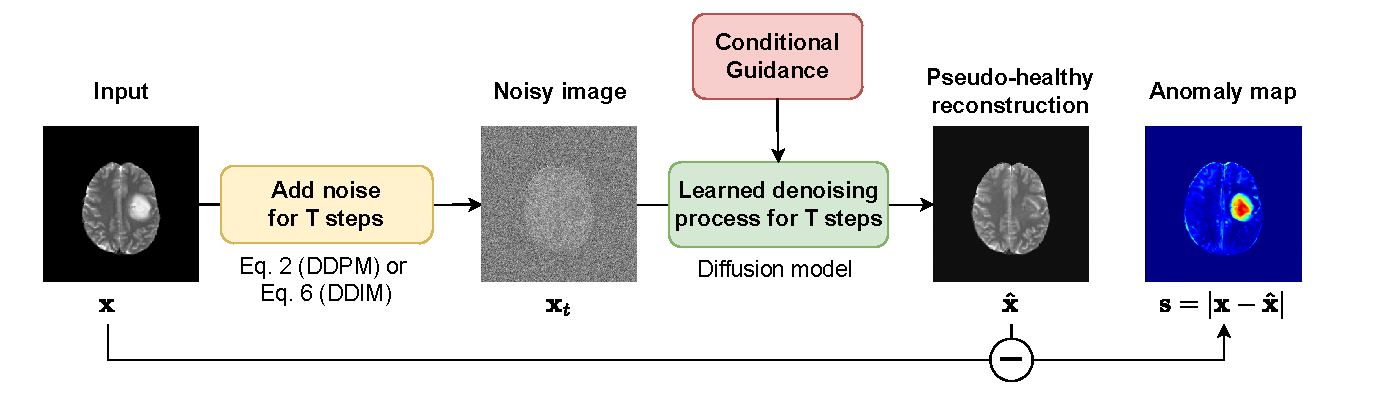
\includegraphics[width=1\linewidth]{figures/uad-overview.pdf}
    \caption[Overview of reconstruction-based UAD]{Overview of reconstruction-based anomaly segmentation with diffusion models. During training, the model learns the distribution of healthy dataset. At inference, we translate an input image to its pseudo-healthy counterpart $\hat\rvx$. The pixel-wise anomaly score map is given by the difference between input and output $D_p = |\rvx - \hat\rvx|$. Figure from \cite{berceaDDPMforMedicalImagesStudy2024}}
    \label{fig:general-uad-diffusion-methods}
\end{figure}

In reconstruction-based \ac{UAD}, a model is trained exclusively on healthy data and, during inference, attempts to generate a pseudo-healthy version of the input image. The core assumption is that since the model has only seen healthy examples during training, it will fail to accurately reconstruct pathological regions while still producing realistic healthy structures. The discrepancy between the input and its pseudo-healthy reconstruction is used to generate a residual map, where high error values indicate potential anomalies. The residual error map is often quantified using the pixel-wise $l$1-error: $D_p = | \rvx - \hat\rvx |$. \ac{GMs} known for their impressive ability to synthesize realistic images, have become prominent tools in this domain. In particular, \ac{VAE} \cite{zimmerer2019VAE-UAD} and \ac{GAN} \cite{fAnoGAN} have been explored, as well as their variants. Recently, \ac{DMs} have shown promise as generative models for \ac{UAD}, due to their ability to produce high resolution synthesized images with accurate inpainting \cite{pinaya2022fastUAD-DDPM, wolleb2022DDPM-weaksupervise, behrendt2025cDDPM}. \cref{fig:general-uad-diffusion-methods} shows an overview of anomaly segmentation task with diffusion models. Nevertheless, reconstruction-based \ac{UAD} methods in general and diffusion models in particular face some critical challenges, mainly:

\begin{description}
    \item[Reconstruction quality]: even though generative models can produce very high quality samples, it is very unlikely that we can achieve near-exact reconstruction images, even those of healthy subjects. This introduces many false positive regions in our anomaly map, specially small errors in the background and around sharp edges of the object. This underlines the importance of developing models that can distinguish between residual errors caused by anomalies and those caused by model limitations.
    
    % As a consequence, selecting an appropriate threshold remains a critical and ongoing challenge for binarizing the anomaly score map to have accurate segmentation without false positive. 
    
    \item[Structure preservation]: in diffusion model, we gradually add noise to input image (\emph{forward process}) and remove them to recover healthy image (\emph{denoise process}). The quantity and quality of noise added to image plays a crucial role in diffusion process, and this aspect is well studied in the literature. \cite{behrendt2025cDDPM} highlight that a key challenge is to limit the reconstruction to healthy brain anatomy. On the one hand, we want to avoid models with limited reconstruction accuracy, which produce imperfect reconstructions everywhere. On the other hand, models that generate highly accurate reconstructions tend to perform a "copy task", resulting in unhealthy structures still reflected in the pseudo-healthy reconstructions. \cite{autoDDPM} refer to this as the \emph{noise paradox}, which states that adding too much noise can destroy not only the anomalous regions but also the healthy structures of the brain. However, adding too little noise can preserve the structure but fail to corrupt the anomaly region, resulting in pseudo-healthy reconstructions that still contain unhealthy structures. 

    \item[Thresholding anomaly score]: Using a trained model, we can produce residual maps that can be interpreted as anomaly scores at both the pixel level and the image level. For anomaly segmentation task, a threshold is required to binarize the score map. At the image level, the goal is to determine a threshold that separates healthy subjects from anomalous ones based on their anomaly scores. However, selecting an appropriate threshold remains an ongoing challenge in \ac{UAD}. Most existing methods in the literature employ greedy algorithms to search for the optimal theoretical threshold based on evaluation metrics (e.g., AUROC, AUPRC). This approach, however, requires a test dataset with fully labeled images and ground-truth segmentations, which violates the principle of unsupervised learning. Other approaches either rely on fixed, predefined threshold values or use quantiles (e.g., the 95th or 97th percentile) of the training or test dataset. In general, selecting an appropriate threshold is challenging and can vary between datasets and applications.
\end{description}

\section{Longitudinal data modeling}
\label{sec:introduction-tdm}

In the context of \ac{UAD} in MRI images, longitudinal data represents repeated MRI scans of a patient at different time points. Unlike timeseries, the number of observations of a single patient is relatively small, and their frequency can be sparse due to patient dropouts, irregular follow-up intervals, and varying lengths of observation periods. Moreover, the complexity of patient metadata, such as age, sex, and disease stage, also affects the progression of disease in different ways. Therefore, we need a solution that can effectively capture both cohort-level (population-wide) and subject-level (individual) trajectories. In recent study, \cite{yangSurveyDiffusionModelsSpatioTemporal2024} show that spatio-temporal diffusion models have achieved state-of-the-art results across many modalities, including images, speech, video, and time series. However, the application of diffusion models to longitudinal data analysis, particularly for MRI anomaly detection, remains underexplored.

Existing literature on longitudinal diffusion models has largely focused on data imputation. However, these approaches rarely exploit the temporal dimension to strengthen spatial anomaly detection. We aim to analyze image sequences across different time points and fuse their information to improve detection and localization of anomalies. This approach can help identify anomalies at earlier stages (reducing false negatives) while filtering out nonpersistent anomalies (reducing false positives). Furthermore, we aim to predict missing observations using the available data and use these imputed images as additional information to improve anomaly localization in future scans.

Our project is inspired by recent advances in longitudinal modeling. \cite{SautyLongitudinalVAE2022} successfully combined a linear mixed-effects model with a \ac{VAE}. In their approach, temporal dependencies are imposed in the latent space of the \ac{VAE}. The mixed-effects model is used to capture the progression of biomarkers in Alzheimer's patients, while spatial variance is learned through the standard \ac{VAE}. By jointly training these two components, their framework demonstrates the ability to model both spatial and temporal aspects in a unified manner. One major difference between these models and diffusion models is that, in \ac{VAE} and normalizing flow frameworks, each observation $\rvx$ corresponds to a single latent variable $\rvz$. Furthermore, this latent variable is typically chosen to have a lower dimensionality, $d \ll D$. In contrast, in diffusion models, each $\rvx$ is associated with a sequence of latent variables $\rvz_t$ that have the same dimensionality as $\rvx$, making it more challenging to impose a temporal structure.

\section{Problem setting}

In this section, we present our problem setting and notations, and we outline the main challenges that we will try to address in this internship. Let ${\rmX^i_{1 \leq i \leq N}}$ be our set of observed $N$ individuals through time, assumed sampled \textit{i.i.d.} from an unknown distribution $p$ that does not depend on $i$. Each patient $i = 1, \ldots , N$ is a sequence of observations through time: $\rvx^i = (\rvx^i_1, \dots, \rvx^i_{L_i})$, where, for each $j, \rvx^i_l \in \mathcal{X} := R^{H \times W \times D}$ is a high dimensional data (2D images or 3D MRI scans) and $L_i$ is the number of observations for a given individual. We note that $L_i \neq L_j$ for any $i \neq j$, which reflects our sparse longitudinal setting: different patients will have different number of observations at different time points. We use notation $L$ to denote longitudinal time point to distinguish from the time step $T$ of diffusion models. 

Given a training set $\mathbf{\mathcal{H} = \{X^{H,i}\}}$ of healthy subjects, our goal is to learn the underlying distribution $q(\rvx^{H, i}_j)$ of each individual sample at any given time. At inference, an anomaly sample $\rvx^{A, i}_j$ is input to our model to produce a pseudo-healthy reconstruction $\hat\rvx^{PH, i}_j$ that follows healthy distribution $q_{\theta}(\rvx^{H, i})$ the network estimates. A residual map is calculated as the difference between original image and its reconstruction $|\rvx - \hat\rvx|$. We will refer to this initial residual map as our pixel-level distance $D_p$ (which can be used for anomaly segmentation). Later on, we will introduce an additional feature distance $D_f$ that focuses more on perceptual difference between two images. 

Our project aims to address some main challenges outlined in \cref{sec:introduction-sdm} and \cref{sec:introduction-tdm}. Our main contributions in this project are summarized as follows: 

\begin{itemize}
    \item Reconstruction quality: we improve the generative power of the diffusion model by enhancing the quality of the conditioning information injected into it. This helps guide the denoising process closer to the true distribution of the input. Secondly, by applying the appropriate noise level, we seek to preserve as much structural detail as possible while ensuring that anomaly regions are fully corrected.
    \item Pixel anomaly score: we introduce feature attention module to combine raw pixel distance with feature distance to further refine our residual map, and eliminate false positive caused by the model errors.
    % We use notation $\rvs$ to denote the anomaly score map, with $\rvs^{pixel}$ and $\rvs^{img}$ represent anomaly score at pixel level and image level, respectively. 
    % \item Image anomaly score: from the pixel anomaly map, we want to find another function to assign a single image anomaly score $\rvs^{img} = \mathcal{F}^{img}(\rvs^{pixel})$. Similarly, this image-level score needs to be thresholded due to the problem of reconstruction quality. 
    \item We employ an automatic thresholding algorithm to remain fully consistent with the unsupervised learning framework.
    \item We incorporate the temporal structure of data to improve the reliability of the spatial diffusion model. Our temporal smoothing module is used to fuse and capture information across different time points. 
    \item When considering the temporal dimension separately, we apply a temporal-aware diffusion model that captures the progression of healthy subjects and generates follow-up images from any given baseline image.
\end{itemize}

% \subsection{Related works}

% \subsubsection{Conditional diffusion models}

% Our project is inspired by recent advances in longitudinal modeling. \cite{SautyLongitudinalVAE2022} successfully combined a linear mixed-effects model with a \ac{VAE}. In their approach, temporal dependencies are imposed in the latent space of the \ac{VAE}. The mixed-effects model is used to capture the progression of biomarkers in Alzheimer's patients, while spatial variance is learned through the standard \ac{VAE}. By jointly training these two components, their framework demonstrates the ability to model both spatial and temporal aspects in a unified manner. One major difference between these models and diffusion models is that, in \ac{VAE} and normalizing flow frameworks, each observation $\rvx$ corresponds to a single latent variable $\rvz$. Furthermore, this latent variable is typically chosen to have a lower dimensionality, $d \ll D$. In contrast, in diffusion models, each $\rvx$ is associated with a sequence of latent variables $\rvz_t$ that have the same dimensionality as $\rvx$, making it more challenging to impose a temporal structure.

% Motivated by the same principle, \cite{ca23LongitudinalNormalizingFlow} use normalizing flow to model the dependencies between observation through time. 



\chapter{Background}
\label{chap:background}

This chapter provides an overview of the mathematical background of diffusion models. We first discuss denoising probabilistic diffusion models in \cref{sec:ddpm}, which form the theoretical foundation for modern diffusion-based generation. Next, we introduce denoising diffusion implicit models (DDIMs) in \cref{sec:ddim}, that uses a non-Markovian process to accelerate the sampling process of the original diffusion models. Finally, we cover the principle of guided diffusion models in \cref{sec:guided-dms}, which uses conditions or contexts to steer the generation process, enabling more controlled and targeted outputs.

\minitoc

\section{Denoising Probabilistic Diffusion Models}
\label{sec:ddpm}

\newcommand{\ExpMp}[2]{\mathrm{Exp}^{\rmM}_{#1, t}(#2)}
\newcommand{\tangentM}{\rmT_{\rvp}\rmM}

\ac{DDPMs} \cite{hoDDPM} are generative models aim to learn a probability distribution $p_{\theta}(\rvx)$ that closely resembles the real data distribution $q(\rvx)$. In diffusion-based generative models learn, we gradually add noise to our original clean image, each step will slightly corrupt the image until it becomes almost featureless distribution. Normally, we choose the noise so that at the end of the diffusion process, we end up with a normal distribution $\gN(0, \rmI)$, which is easy to sample from in our generative process. \ac{DDPMs} is composed of two processes: \textit{forward process} and \textit{backward process} (generative process).

\subsubsubsection{Forward process} In the forward process, we gradually add noises to our input $\rvx \sim q(\rvx)$ to generate a series of noisy images $(\rvx_1, \rvx_2, ..., \rvx_T)$ for many time steps $T$. The noise level $t$ of an image $\rvx_t$ is predefined by a noise schedule $\beta_t \quad t \in [1, T]$, which is originally implemented as a linear schedule going from $\beta_0 = 10^{-4}$ to $\beta_T = 0.02$ in \cite{hoDDPM}. The forward process is a non-homogenous Markov chain process, with the following kernel transition: 
\begin{align}
    q(\rvx_{1:T} \mid \rvx_0) &:= \prod_{t=1}^{T} q(\rvx_t \mid \rvx_{t-1}) \\
    q(\rvx_t \mid \rvx_{t-1}) &= \gN\left(\rvx_t;\, \sqrt{1 - \beta_t}\, \rvx_{t-1},\, \beta_t I\right) \label{eq:forward} \quad \text{for } t = 1,\ldots,T
\end{align}

\cite{hoDDPM} defines $\alpha = 1 - \beta_t$ and $\bar\alpha = \prod_{s=1}^{t} \alpha_t$, and the forward process has a special property that we can use to jump directly from $\rvx_0$ to any noisy $\rvx_t$ given a time step $t$ \footnote{This is referred to as the Nice property of diffusion model. See math derivation from \cite{soto2024ddpmLecture}}:
\begin{align}
 q(\rvx_t | \rvx_0) = \gN(\rvx_t; \sqrt{\bar\alpha}\rvx_0, (1 - \bar\alpha_t) \rmI) \label{eq:q-xt} 
\end{align}
Using the reparameterization trick, we can express $\rvx_t$ as: 
\begin{align}
    \rvx_t = \sqrt{\bar\alpha} \rvx_0 + \sqrt{\bar\alpha_t} \epsilon \quad \mathrm{with} \quad \epsilon \sim \gN(0, \rmI) \label{eq:xt-from-x0}
\end{align}

We see that with large enough $T$ (normally $T=1000$), $\bar\alpha_t \to 0$, and $\rvx_t$ converge to a Gaussian distribution $\gN(0, \rmI)$. With a learned reversed process, we can sample from this normal distribution to generate new image from the original distribution. 

\subsubsubsection{Generation process} for image generation, we start from a random variable $\rvx_T \sim \gN(0, \rmI)$ and the generation process is given by: 
\begin{align}
    p(\rvx_{0:T}) &= p(\rvx_T) \prod_{t=1}^T{p_{\theta}(\rvx_{t-1} | \rvx_t)} \\
    \mathrm{with} \quad p_{\theta}(\rvx_{t-1} \mid \rvx_t) &= \gN (\rvx_{t-1}; \mu_{\theta}(\rvx_t, t), \Sigma_{\theta} (\rvx_t, t)) \label{eq:ddpm-sample}
\end{align}

The denoising network $p_{\theta}$ is learned by optimizing model parameters $\theta$ to predict $\rvx_{t-1}$ from $\rvx_t$, for each $t \in [1 ... T]$. This is equivalent to gradually remove noise at each time step, so we can generate noise-free image $\hat{\rvx}$ at $t = 0$. Instead of learning both $\mu_{\theta}$ and $\Sigma_{\theta}$, \cite{hoDDPM} show that by conditioning the true posterior on $\rvx_0$, we can fix $\Sigma_\theta(\rvx_t, t) = \Sigma(t)$, and the mean $\mu_\theta$ can be derived using a noise prediction network $\epsilon_{\theta}$ \cite{soto2024ddpmLecture}: 
\begin{align}
    \Sigma_\theta(\rvx_t, \rvx_0, t) &= \Sigma(t) = \frac{1 - \alpha_{t-1}}{1 - \alpha_t} \, \beta_t \mathbf{I} \\
    \mu_{\theta} (\rvx_t, \rvx_0, t) &= \frac{1}{\sqrt{\alpha_t}} ( \rvx_t -\frac{\beta_t}{\sqrt{1 - \bar{\alpha}_t}} \, \epsilon_{\theta} (\rvx_t, t)) \label{eq:epsilon}
\end{align}

\subsubsubsection{Learning objective}: $\epsilon_\theta (\rvx_t, t)$ in 
\cref{eq:epsilon} is the output of a time conditioned network, which \cite{hoDDPM} use UNet architecture to predict the noise added to the original image $\rvx_0$ at time $t$. The network is trained with loss function: 
\begin{align}
    \mathcal{L} (\theta) &= ||\epsilon - \epsilon_{\theta} (\rvx_t, t) ||^2 = || \epsilon - \epsilon_{\theta}(\sqrt{\bar\alpha} \rvx_0 + \sqrt{\bar\alpha_t} \epsilon)||^2 \label{eq:loss-ddpm} \\
    \mathrm{where} &\quad \rvx_0 \sim q(\rvx_0), \quad t \sim \mathrm{Unif}[1, T], \quad \epsilon \sim \gN(0, \rmI) \nonumber
\end{align}

\section{Denoising Diffusion Implicit Models}
\label{sec:ddim}

\subsubsubsection{DDIM sampling scheme}: one disadvantage of \ac{DDPMs} is during inference, we have to go through each step in reverse $t \in [T ... 0]$, and with large $T$ comes with longer inference time. \ac{DDIMs} \cite{songDDIM} accelerate \ac{DDPMs} by introducing a non-Markovian sampling process $q_{\sigma}(\rvx_{t-1} \mid \rvx_t, \rvx_0)$. \ac{DDIMs} defines a new variance schedule $\sigma$ that is chosen to have the same marginal distribution as in \cref{eq:q-xt}. So the training procedure and objective stay the same as in \ac{DDPMs}, but only the sampling process is different. Based on \cref{eq:xt-from-x0}, we can predict noise-free observation $\hat\rvx$ as: 
\begin{align}
    \hat\rvx_0 = f_{\theta}(t, \rvx_t) = \frac{\rvx_t - \sqrt{1 - \alpha_t} \cdot \epsilon_{\theta}(\rvx_t, t)}{\sqrt{\alpha_t}} \label{eq:pred-x0-from-xt}
\end{align}

\cite{songDDIM} generalize the \ac{DDPMs} sampling scheme as: 
\begin{align}
    \rvx_{t-1} = \sqrt{\alpha_{t-1}} \, f_{\theta}(t, \rvx_t) + \sqrt{1 - \alpha_{t-1} - \sigma_t^2} \, \epsilon_{\theta}(\rvx_t, t) + \sigma_t \, \epsilon \label{eq:ddim-sample-xt}
\end{align}

where $\epsilon \sim \gN(0, \rmI)$ and $\sigma_t$ controls the stochasticity of the sampling process. For \ac{DDPMs}, we choose $\sigma_t = \sqrt{(1 - \bar{\alpha}_{t-1})/(1 - \bar{\alpha}_t)} \sqrt{1 - \bar{\alpha}_t/\bar{\alpha}_{t-1}}$, thus \ac{DDPMs} will always have a stochastic element in its sampling step \footnote{This is also why we have to perform \ac{DDPMs} sample step by step instead of deriving $\rvx_0$ directly from $\rvx_T$ by reversing \cref{eq:xt-from-x0}. \cite{soto2024ddpmLecture} show both the mathematical and intuitive reasons behind this}. On the other hand, if we set $\sigma_t = 0$, we have an extreme case of deterministic DDIM sampling process, which means that $\rvx_{t-1}$ is fully determined given $\rvx_0$ and $\rvx_t$. Formally, the deterministic DDIM sampling scheme is defined as: 
\begin{align}
    p_{\theta}(\rvx_{t-1} \mid \rvx_t) &= \mathcal{N} (\sqrt{\alpha_{t-1}} \, f_{\theta}(t, \rvx_t) + \sqrt{1 - \alpha_{t-1}} \, \epsilon_{\theta}(\rvx_t, t), 0)\label{eq:ddim-posterior-deterministic} \\
    \rvx_{t-1} &= \sqrt{\alpha_{t-1}} \, f_{\theta}(t, \rvx_t) + \sqrt{1 - \alpha_{t-1}} \, \epsilon_{\theta}(\rvx_t, t) \label{eq:ddim-sample-deterministic}
\end{align}

\subsubsubsection{DDIM noise encoding}: As derived in \cite{songDDIM}, \cref{eq:ddim-sample-deterministic} can be viewed as the  Euler method to solve an ordinary differential equation (ODE). Consequently,  we can reverse the generation process by using the reversed ODE. With enough discretization steps, we can encode $\rvx_{t+1}$ given $\rvx_t$ with: 
\begin{align}
    \rvx_{t+1} = \rvx_t + \sqrt{\bar\alpha_{t+1}} \left[ \left(\sqrt{\frac{1}{\bar\alpha_t}} - \sqrt{\frac{1}{\bar\alpha_{t+1}}} \right) \rvx_t + \left( \sqrt{\frac{1}{\bar\alpha_{t+1}} - 1} - \sqrt{\frac{1}{\bar\alpha_t} - 1}\right) \epsilon_{\theta} (\rvx_t, t) \right] \label{ep:ddim-encode}
\end{align}

By applying \cref{ep:ddim-encode} for $t \in \{1, ..., T-1\}$, we can encode a clean image into a noisy image $\rvx_T$. We refer to this $\rvx_T$ as \emph{stochastic subcode} of $\rvx_0$, and \cite{DiffAE} show that this stochastic encoding process stores fine-grain detail about $\rvx_0$. Starting from this stochastic subcode, we can then decode it using \cref{eq:ddim-sample-xt} to have a near-exact reconstruction of $\rvx_0$ \cite{DiffAE, lozuponeLDAE2025, wolleb2022DDPM-weaksupervise}.

\section{Guided diffusion models}
\label{sec:guided-dms}

Diffusion models described in \cref{sec:ddpm} is designed to generate unconditional images, but many downstream tasks require generating images that adhere to a specific condition. Given an input image $\rvx$ and its corresponding class or context $\rvy$, we want to train a diffusion model that can generate images belong to a given class $\rvy$ \footnote{I slightly abuse the term "class" here to align with common usage in the literature, even though in the UAD setting we typically do not have access to the true class label of the anomalous subject. Throughout the rest of this report, the terms "class" and "context" will be used interchangeably.}. In this section, we briefly discuss several techniques that are used to guide the diffusion process. 

\subsubsubsection{Gradient guided diffusion}: \citeauthor{dhariwalDiffusionModelsBeatGAN2021}~\cite{dhariwalDiffusionModelsBeatGAN2021} incorporate the class guidance into the denoising process by training a separate classifier network $C$ to distinguish between class labels. The network $C(\rvy \mid \rvx_t, t)$ is trained at every noise step $t$ with corresponding noisy image $\rvx_t$ obtained by \cref{eq:xt-from-x0}. During DDIM sampling, the predicted noise in \cref{eq:ddim-sample-deterministic} is modified as: 
\begin{align}
    \hat{\epsilon}_{\theta} = \epsilon_{\theta} (\rvx_t, t) - s \sqrt{1 - \bar\alpha_t} \nabla_{\rvx_t} \log C(\rvy \mid \rvx_t, t) \label{eq:class-guide-epsilon}
\end{align}

where $s$ is a parameter controls the strength of the guidance, and $\nabla_{\rvx_t} \log C(\rvy \mid \rvx_t, t)$ can be interpreted as log gradient of the likelihood of class $\rvy$ given a noisy image $\rvx_t$. From probabilistic model perspective, by taking a step in the opposite direction of this gradient, we can move toward region with higher density, and theoretically that will allow us to arrive at the mode of the true distribution $p(\rvy \mid \rvx_t)$. In the context of diffusion sampling process, this steers the generation of $\rvx_{t-1}$ toward the desire class $\rvy$. We note that this highlights the connection between diffusion models and score-based models \cite{songScoreBasedGenerativeModeling2021}, and we can reformulate $\epsilon_{\theta}$ in \cref{eq:ddim-sample-xt} to be a score-based function, which estimated the deviation should happen at each time step $t$ to arrive at a clean image $\rvx_0 \sim q(\rvx)$, as shown in \cite{DDAD, luoUnderstandingDiffusionModels2022}: 
\begin{align}
    \nabla_{\rvx_t} \log p_{\theta} (\rvx_t) = - \frac{1}{\sqrt{1 - \bar{\alpha}_t}} \epsilon_{\theta} (\rvx_t, t) \label{eq:connection-epsilon-score-func}
\end{align}

\subsubsubsection{Classifier-free guided diffusion}: one major disadvantage of gradient guidance method is that we need to train an additional class condition network $C(\rvy \mid \rvx_t, t)$, and output quality depends on the performance of the classification network, introducing potential bias \cite{berceaDDPMforMedicalImagesStudy2024}. For the network to learn effectively, For the network to learn effectively, we need to train it for each class $\rvy$, at every noise level$t$, and for every $\rvx_0$. This approach is computationally expensive. There are some alternative methods that leverage this score-based function without needing to train a classifier network. One approach is to inject the context directly into the UNet to provide guidance for the network. Formally, given a noisy image $\rvx_t$ at time step $t$ and a context $\rvy$, we want to update our noise prediction output from \cref{eq:epsilon} become $\epsilon_{\theta}(\rvx_t, t, \rvy)$ to incorporate this information.
 Our loss function in \cref{eq:loss-ddpm} becomes:
\begin{align}
    \mathcal{L} (\theta) &= || \epsilon - \epsilon_{\theta}(\rvx_t, t, \rvy)||^2 \label{ep:loss-cond-ddpm}
\end{align}

There are several methods for implementing conditioning mechanisms. Some earlier approaches use the input $\rvx$ directly as context and concatenate this information with the noisy image $\rvx_t$. In this implementation, the context is \emph{spatial context}, i.e. $\rvy \in \mathbb{R}^{h \times w}$. However, this strategy has the potential drawback of revealing the target to the network, since subtracting $\rvx$ from $\rvx_t$ yields the exact noise that was added. To address this, more recent approaches use \emph{non-spatial context} $\rvy \in \mathbb{R}^d$, which is generated by a semantic encoder network. LDM \cite{rombachLDM} employs a cross-attention module to inject context at every step of the UNet, while cDDPM \cite{behrendt2025cDDPM} concatenates the context with the time embedding. 

% \begin{itemize}
%     \item DDAD \cite{DDAD} 
% \end{itemize}

% \subsection{Longitudinal data analysis}

% \subsubsection{Reimannian manifold}

% We made the hypothesis that the data of interest belong to a particular subspace of the feature space, that individual trajectories are described by curves on this subspace and that the repeated observations are points on these curves. This subspace is thus central to the disease modeling as it entirely defines the space of possible measurements and consequently the individual spatiotemporal trajectories.

% \begin{description}
%     \item[Manifold]: is a topological space for which each point presents a neighborhood that is homeomorphic to the Euclidean space. To this extend, there exist collections of mapping (\emph{atlas}) that transform local neighborhood around point $\mathbf{p}$ to a linear space.
    
%     \item[Tangent space]: for any point $\rvp$ in a smooth manifold $\rmM \in \sR^{n}$, its \emph{tangent} space $\rmT_{\rvp}\rmM$ is a linear approximation of local \emph{region} around $\rvp$

%     \item[Geodesic]: The geodesics correspondes to the shortest path betwen two points on the manifold $\rmM$, similar to a straight line in Euclidean space. Given $\gamma : I \in \sR \to \rmM$, is a geodesic of $\rmM$ if $\nabla_{\dot\gamma}\dot\gamma = 0$, i.e. a smooth curve with zero acceleration. $I$ is an interval of real number, which represents the parameter domain — usually time or some abstract "path parameter" along the curve. $\gamma$ is a function that maps $t \in I$ to a point $\gamma(t)\rmM$. It is a parametrized curve that traces out a path on the manifold $\rmM$. 
    
%     Intuition about $\gamma$: Think of $\gamma(t)$ as a particle moving along the surface of $\rmM$ as time $t$ varies:
%     \begin{itemize}
%         \item You input a time  or parameter $t$
%         \item You get a point on the manifold $\rmM$

%         \item The \emph{image} of $\gamma$ is defined as: $\mathrm{Im}(\gamma) = \{\gamma(t) \in \rmM | t \in I\}$
%     \end{itemize}

%     \item[Exponential map]: at any point $\rvp$ in $\rmM$ and a vector $\rvv \in \tangentM$, the mapping $\ExpMp{\rvp}{\rvv}$ is Riemannian exponential map, that is the point we can reach at time $t$ from $\rvp$ by taking a sequence of steps from $\rvp$ with velocity $\rvv$. 

%     \item[Parallel-transport]: 
% \end{description}

% \subsubsection{Spatiotemporal disease progression modeling}

% \begin{align}
%     \rvy_{i,j} &= \eta^{\rvw_i}(\gamma_0, \psi_i(t_{i,j})) + \varepsilon_{i,j} \label{eq:mix-effect} \\
%     \psi_i(t_{i,j}) &= t_{i, j} \to \alpha_i \left( t - \tau_i - t_0 \right) + t_0 \label{eq:temporal-effect} \\
%     \psi_i(t_{i,j}) &= t_{i, j} \to \rvv_0 e^{\xi_t} \left( t - \tau_i \right) + t_0 \label{eq:temporal-effect2}\\
%     \eta^{\rvw_i} (\gamma_0, t) &:= \mathrm{Exp}_{\gamma_0(t)}(P_{\gamma_0, t_0, t}(\rvw_i)) \label{eq:spartial-effect} \\
%     \gamma_0: I \in \sR \to \rmM \in \sR^N &:= (\rvp_0, t_0, \rvv_0) \label{eq:fix-effect} \\
%     \rvp_0 &= \gamma_0 (t_0) \\
%     \rvv_0 &= \dot\gamma_0 (t_0) 
% \end{align}

% \href{https://leaspy.readthedocs.io/en/latest/mathematics.html#riemanian-framework}{leaspy documentation} that explains: 
% \begin{description}
%     \item[Population trajectory and fix effect]: The \textbf{fixed-effects} of the model are the parameters of the average geodesic given in \cref{eq:fix-effect}. This population trajectory is fully described by its initial condition: the point \(\rvp_0\) on the manifold, the time-point \(t_0\) and the velocity \(\rvv_0\). 

%     \item[Individula trajectory with spartial random effects] is defined by \emph{space shift} $\rvw_i \in \tangentM$ in \cref{eq:spartial-effect}. It represents the direction in which the group-average trajectory is shifted to approximate the data $(\rvy_{i,j})_{1 \leq j \leq k}$ of the $i$-th individual. We note that $\rvw_i$ is only one vector defined at the starting point $(\rvp_0, t_0)$, and is parallel-transport along the curve $\gamma_0$ at any given $t$. This gives us the directional vector that should happen at any $t$ to derive the individual curve from population curve. The resulting vector writes $P_{\gamma_0, t_0, t} (\rvw_i)$. The exponential map of the collection of these vector writes $\mathrm{Exp}_{\gamma_0 (t)} (P_{\gamma_0, t_0, t} (\rvw_i))$ defines the individual trajectory $\eta^{\rvw_i} (t)$.  

%     \item[Individual trajectory with temporal random effects] in \cref{eq:temporal-effect} is defined by \emph{time shift} $\tau_i \in \sR$ and \emph{accelerator shift} $\alpha_i \in \sR$. For each individual patient $i$, $\psi_i(t_{i,j})$ is the temporal reparameterization that represents patient timeline. It transforms the individual observation time point from chronological time (real patient age) to disease time point. This transformation accounts for difference between individual reference time (\emph{onset age}) $\tau_i$ and population reference time $t_0$, and the speed at which a patient disease progresses $\alpha_i$. If a patient starts to have symptoms of the disease earlier (resp. later) than the average population, it impacts the initial condition with $(\tau_i - t_0) > 0$ (resp. $(\tau_i - t_0) < 0$). Similarly, if a patient has a faster (resp. slower) disease progression, the individual trajectory is impacted by acceleration factor $\alpha_i > 0$ (resp. $\alpha_i < 0$). In line with \cite{SautyLongitudinalVAE2022}, we can rewrite $\alpha_i = e^{\xi_i}$ with $\xi_i$ as individual log speed factor in \cref{eq:temporal-effect2}, similar to the implementation in the \texttt{leaspy} package. \footnote{List of \texttt{leaspy} notations and DAG names can be found on \href{https://leaspy.readthedocs.io/en/latest/notations.html}{https://leaspy.readthedocs.io/en/latest/notations.html}}. These two parameters $(\xi_i, \tau_i)$ form the temporal part of the \textbf{random effects} and explain the temporal variability in our dataset.  

%     \item[Residual noise]: finally, we denote $\epsilon_{i, j}$ as random noise at time $j$ that the model does not capture. 
% \end{description}



\chapter{Proposed Frameworks for Spatial-Temporal UAD}
\label{chap:sdm}

In this section, we introduce our proposed framework for Spatial-Temporal unsupervised anomaly detection, comprises two main modules: \ac{SDM} (\cref{sec:sdm}) and Anomaly Detection Module (\cref{sec:fam}). During the training of \ac{SDM}, we remove all temporal dependencies between samples and treat them as \emph{i.i.d} sample. \ac{SDM} accounts only for the spatial representations of the input. At inference, we add back the temporal dependencies using longitudinal module to increase the accuracy of anomaly segmentation. 

\minitoc

\section{Spatial Diffusion Model for pseudo-healthy data generation}
\label{sec:sdm}

\begin{figure}[htbp]
    \centering
    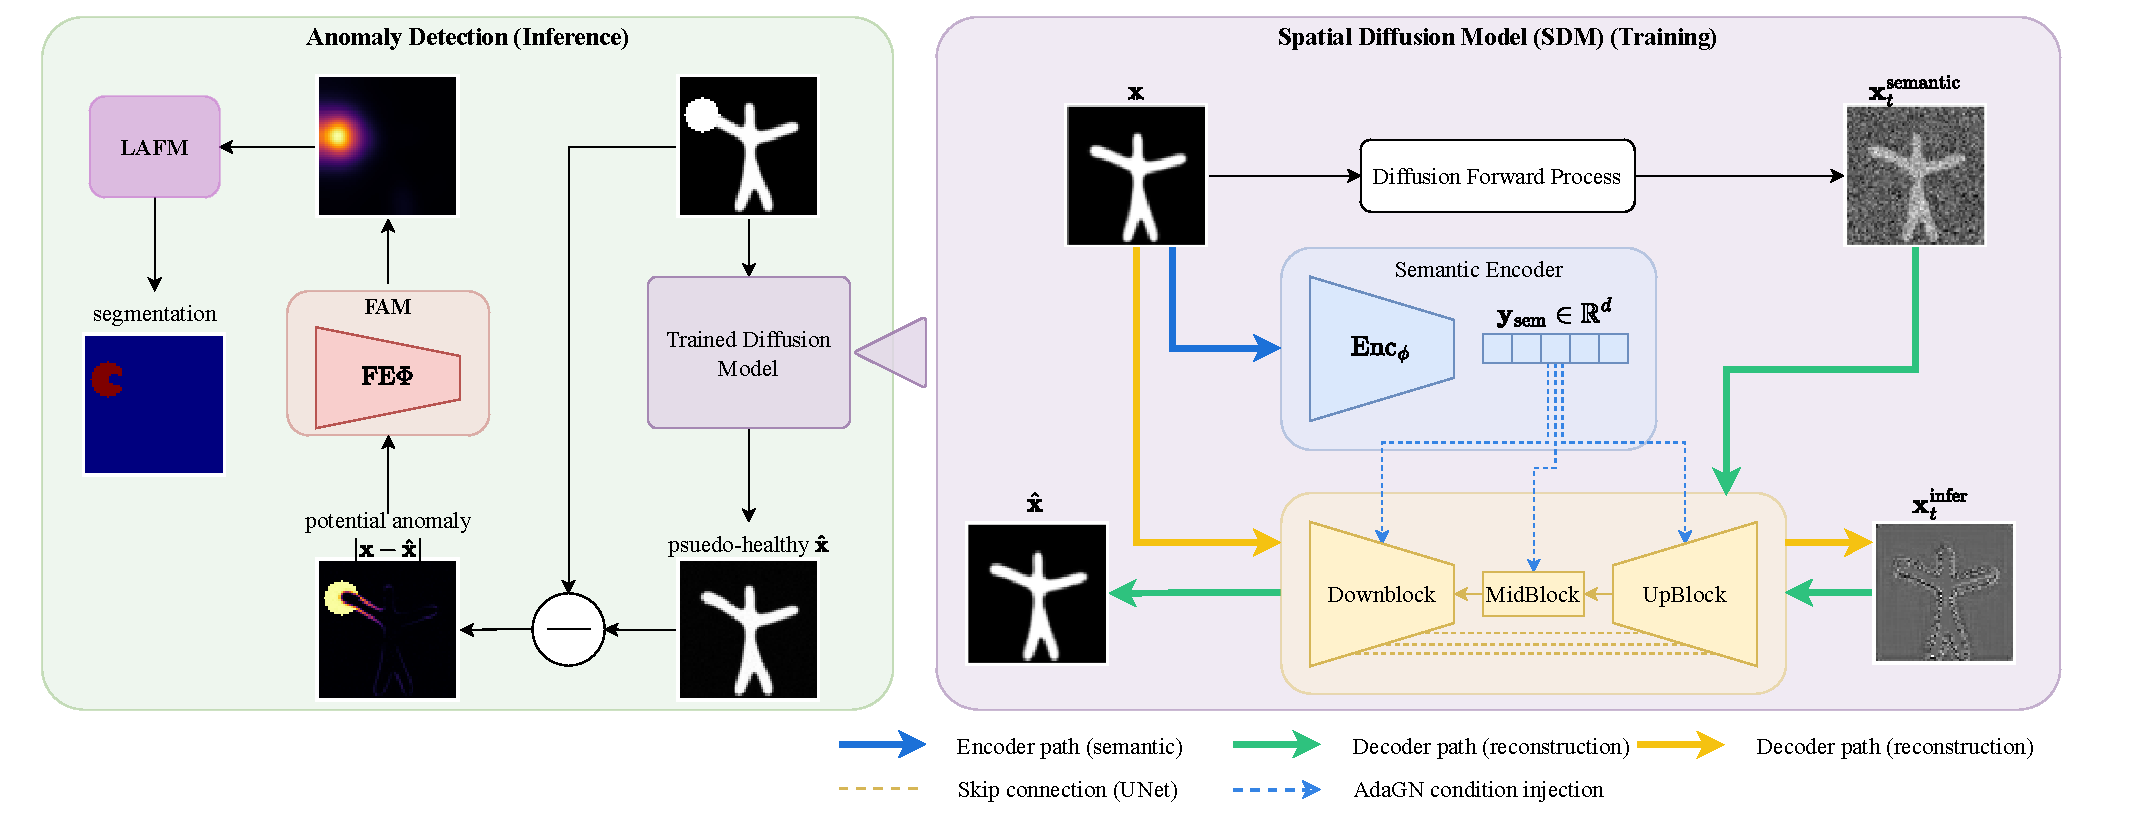
\includegraphics[width=1\linewidth]{figures/model-sdm.pdf}
    \caption[Overview of Spatial-Temporal UAD framework]{Overview of our \ac{SDM} framework for unsupervised anomaly detection using reconstruction-based method. Our model consists of four keys components: (i) \textbf{semantic encoder} extracts a non-spatial representation of input $(\rvx \to \rvy_{\text{sem}})$, (ii) \textbf{denoising UNet} comprises a down block, a middle block and up block with skip connection to concatenate information from down blocks to corresponding up blocks, (iii) \textbf{Feature Attention Module (FAM)}, and (iv) \textbf{Longitudinal Attention Fusion Module (LAFM)}. The semantic representation is injected as conditions into our diffusion process. Conditional diffusion UNet acts as both a stochastic encoder $(\rvx \to \rvx_T^{\text{infer}})$ and a decoder (DDIM denoising step) $(\rvx_T \to \widehat{\rvx})$. During inference, we use trained SDM to reconstruct pseudo-healthy image of input, and potential anomaly map is calculated as residual $|\rvx - \hat{\rvx}|$. We use \ac{FAM} to clean residual map, and \ac{LAFM} module further fuses information from other time points to have final anomaly segmentation.} 
    \label{fig:model-sdm}
\end{figure}

We now introduce the framework of our proposed SDM, with anomaly detection process during inference. Our SDM comprises four keys blocks: a semantic encoder (\cref{sec:method-semantic-encoder}), a denoising UNet (\cref{sec:method-unet}), a \ac{FAM} (\cref{sec:feature-extractor-network}) and a \ac{LAFM} (\cref{sec:method-lafm}). These four components, summarized in \cref{fig:model-sdm}, collectively can address the challenges we outlined in the introduction. We structure the description of SDM into two parts: this section provides a detailed explanation of diffusion model for image reconstruction (training phase). \cref{sec:fam} will discuss anomaly detection during inference phase. In training process, our SDM is designed as a conditional diffusion model that treats each $\rvx^i_l \quad (l = 1, ..., L_i)$ as independent cross-sectional data. To simplify the notation, we omit the superscript $i$ and subscript $l$ from here onward. During inference, we introduce \ac{FAM} and \ac{LAFM} after the denoising process to achieve final anomaly prediction and anomaly segmentation. 

\subsection{Semantic Encoder}
\label{sec:method-semantic-encoder}

The goal of the semantic encoder $\mathrm{Enc}_\phi(\rvx)$ is to summarize an input image into a meaningful non-spatial representation $\rvy_{\text{sem}} \in \mathbb{R}^d$ with enough information to help the decoder $p_\theta(\rvx_{t - 1}|\rvx_t, \rvy_{\text{sem}})$ denoise and predict the output image. We employ ResNet-50 \cite{ResNet50} as our semantic encoder. ResNet-50 has 50 layers, and is built around residual connections that enable stable training of very deep models. It comprises four main residual blocks operating at progressively lower spatial resolutions that capture hierarchical feature representations of the input. We replace the last classifier layer with an MLP that produces a non-spatial representation of the input. Together with time step $t$, $\rvy_{\text{sem}}$ form the condition that we will inject into diffusion UNet. 

\subsection{Diffusion UNet}
\label{sec:method-unet}

The core component of our SDM is denoising UNet module $\epsilon_{\theta}$ with trainable parameter $\theta$, adapted from \cite{dhariwalDiffusionModelsBeatGAN2021}. Given a clean image $\rvx$ and a time step $t$, we add noise to the image using \cref{eq:xt-from-x0}. The time step $t$ controls the amount of added noise and is sampled from $t \sim \mathrm{Uniform}(1 \ldots T )$. When $t=T$, the image $\rvx$ is transformed into pure noise $\rvx_T \sim \mathcal{N}(0, \mathbf{I})$. Subsequently, $\rvx_t$ is passed through the UNet, which predicts the added noise. We condition the backward process on context vector comprises time step and semantic representation $c=(t, \rvy_{\text{sem}})$. Time step is embedded using sinusoidal positional embeddings, originated from \cite{vaswani2023attentionneed}, while semantic representation is the output of our semantic encoder. To provide context $c$ into UNet, we use FiLM-style adaptive group norm (\textrm{AdaGN}), following \cite{dhariwalDiffusionModelsBeatGAN2021}. We formulate our \textrm{AdaGN} operation as: 
\begin{align}
    \mathrm{AdaGN}(\rvh, t, \rvy_{\text{sem}}) = \rvy_{\text{sem}}^s (\rvt_s . \mathrm{GroupNorm}(\rvh) + \rvt_b) + \rvy_{\text{sem}}^b \label{eq:adagn}
\end{align}
% To provide context, we use a semantic encoder to map the original image $\rvx$ to $\rvy_{\text{sem}} \in \mathbb{R}^d$, together with the corresponding time step $t$. The time step is embedded using sinusoidal positional embeddings. Both $t$ and $\rvy_{\text{sem}}$ are injected into the UNet via FiLM-style adaptive group normalization, following \cite{dhariwalDiffusionModelsBeatGAN2021}.

where $\rvh$ denotes the hidden feature map at each level of the UNet. The pairs $[\rvy_{\text{sem}}^s, \rvy_{\text{sem}}^b]$ and $[\rvt_s, \rvt_b]$ are obtained via linear projections of $\rvy_{\text{sem}}$ and $t$, respectively. They represent the \emph{shift} and \emph{scale} parameters applied to the feature maps, effectively adjusting them according to the conditioning signals. This design enables the model to guide the denoising process using high-level semantic codes. Compared to using a cross-attention module as in \cite{rombachLDM}, this approach is simpler, and unlike concatenating $\rvy$ with $t$ as in \cite{behrendt2025cDDPM}, it does not increase the hidden dimensionality of $\rvh$.

The semantic encoder is jointly trained with UNet with updated loss function: 
\begin{align}
    \mathcal{L} (\theta, \phi) &= || \epsilon - \epsilon_{\theta}(\rvx_t, t, \mathrm{Enc}_{\phi}(\rvx)||^2 \label{ep:loss-cond-encoder-ddpm}
\end{align}

We can interpret this training algorithm as forcing the semantic encoder $\mathrm{Enc}\phi$ to capture as much information about $\rvx$ as possible. Theoretically, if $\rvy_{\text{sem}} = \mathrm{Enc}\phi(\rvx) \in \mathbb{R}^d$ retains all the information of the input, we can achieve exact reconstruction \cite{lozuponeLDAE2025}. 

During inference, our trained model can generate a new sample by denoising process using \cref{eq:ddpm-sample}, starting from pure noise $\rvx_T \sim \mathcal{N}(0, \mathbf{I})$. We elevate the sampling process using DDIM sampling scheme, using \cref{eq:ddim-sample-deterministic}. We set $\sigma=0$ to have a deterministic process. It is worth noting that although the training process is performed with $T = 1000$ steps, it is not necessary to reconstruct healthy images from pure noise. In fact, since our main objective is not to generate entirely new images but rather to heal anomalous regions, it is preferable to start decoding from a noise level $t < T$. Using this approach, we preserve some high-level structure of the original image, in contrast to starting from pure noise. The noisy image $\rvx_t$ is obtained by adding noise to $\rvx_0$ with \cref{eq:xt-from-x0}.

\subsection{Stochastic Encoder and Conditional Decoder}

% As shown in \cite{DiffAE, lozuponeLDAE2025}
Here, we provide further insights into our encode and decode processes. We refer to our semantic encoder in \cref{sec:method-semantic-encoder} as \emph{semantic encoder}, which map input into its nonspatial representation. We will refer to $\rvy_{\text{sem}}$ as our \emph{semantic subcode}. In addition, our denoising network $\epsilon_\theta$ plays a dual role in our model. Its main purpose is to act as a \emph{conditional decoder} that can generate healthy images from noisy input. On the other hand, it can also serve as a \emph{stochastic encoder} by using deterministic DDIM sampling scheme. Given a clean image $\rvx$, SDM can encode it to a stochastic subcode using \cref{ep:ddim-encode}. \cite{DiffAE, lozuponeLDAE2025} demonstrates that this stochastic subcode contains fine grain details about $\rvx$ that is not captured by semantic encoder. We note that, unlike the standard noising process \cref{eq:xt-from-x0}, the stochastic subcode does not necessarily follow Gaussian noise, since it retains residual information about the input. We refer to \emph{stochastic subcode} of original image $\rvx$ as $\rvx_t^{\mathrm{infer}}$, and normal noisy image as $\rvx_t^{\textrm{semantic}}$ (or $\rvx_t$) \footnote{We note that in our report, $\rvx_t^{\text{semantic}}$ and $\rvx_t$ are used interchangeably. $\rvx_t^{\text{semantic}}$ is used in the context of comparison with $\rvx_t^{\text{infer}}$ to emphasize the differences, whereas $\rvx_t$ is used elsewhere for the sake of brevity.}, with $t \leq T$. 

% \subsection{Anomaly Detection with SDM}
\section{Unsupervised Anomaly Detection Module}
\label{sec:fam}

% However, this approach faces several challenges when we have to deal with subtle anomaly. First, we will almost never achieve a perfect reconstruction even with healthy images, and the \textit{l1}-distance at pixel level rarely reachs $0$. This often results in false negatives, especially along sharp edges of objects. Second, pixel-wise comparisons can lead to false positives when slight distortions appear in the background, that the UNet model may not learn during training, and hence does not reconstruct accurately during inference. 

In the simplest case, reconstruction-based method relies on pixel wise difference between the original image $\rvx$ and psuedo-healthy reconstructed image $\hat{\rvx}$ to generate the anomaly map, which will be used as our anomaly segmentation. To address the challenges mentioned in \cref{sec:introduction-sdm}, we aim to employ techniques that: (i) ignore small outliers in the background, (ii) discard minor reconstruction errors around object edges, and (iii) emphasize differences within the critical anomaly region (i.e., the region of interest). \cite{zhang2018unreasonableeffectivenessdeepfeatures} introduce the effectiveness of using image features as perceptual metrics, which are robust to minor pixel-level differences that do not alter the overall image structure. Features are sensitive to changes in texture and shape, but can be robust against slight transformation where pixel level distance might fail. We follow method of DDAD \cite{DDAD} that defines anomaly score as combination of both pixel and feature errors. By utilizing both pixel differences and features differences, we can achieve high precision in anomaly localization. We refer to this process that wraps around the feature extractor network as our \ac{FAM}. We discuss the methodology of \ac{FAM} in the section below. 

%Based on this reasoning, PatchCore \cite{PatchCoretotalrecall} introduce anomaly score system that is entirely relies on feature distances. It uses locally aware patch features to build a memory bank of reference features extracted from healthy images. While PatchCore achieves state-of-the-art performance with $99.1\%$ AUROC without pixel level erros,  we think they are still good indicators for anomaly localization. 

\subsection{Feature Attention Module}
\label{sec:feature-extractor-network}

\paragraph{Anomaly score as combination of feature distances and pixel distances} Given an input image $\rvx$, and it's psuedo-healthy reconstruction $\hat{\rvx}$, we define a pixel-wise distance function $D_p$ and a feature-wise distance function $D_f$ to derive the anomaly heatmap. $D_p$ is calculated based on the $\gL_1$ norm in pixel space. At the feature level, we use adaptive average pooling to spatially smooth each individual feature map. Feature distance $D_f$ is then calculated as a cosine-similarity. Formally we have: 
\begin{align}
D_p(\rvx, \hat{\rvx}) &= \mathcal{L}_1(\rvx - \hat{\rvx}) \\
D_f(\rvx, \hat{\rvx}) &= \sum_{j \in J} \operatorname{Interp}\left(1 - \cos\left(\Phi_j(\rvx), \Phi_j(\hat{\rvx})\right)\right)
\end{align}

where $\Phi$ is a pre-trained feature extractor network and $j$ refers to the level (or stage) that we want to extract feature from, and $\operatorname{Interp}$ is the interpolation operator of feature maps to match input's resolution. We note that for each feature level $j$, the cosine similarity is calculated along channel dimension and for each pixel. Formally, we have $\rvx, \hat\rvx \in \mathbb{R}^{h \times w}$, $\Phi_j(\rvx), \Phi_j(\hat\rvx)$, and $\mathrm{cos}(., .) \in \mathbb{R}^{h_j \times w_j}$, with $h_j, w_j$ are dimensions of feature map $j$. 

We utilize our trained semantic encoder $\mathrm{Enc}_{\phi}$, and we train a copy of it as feature adaptation step. We give detail about this step in section \ref{sec:feature-extractor-network}. We follow the convention with existing literatures for ResNet-like architecture, so that $j \in \{1, 2, 3, 4\}$ indicating the final output of respective spatial resolution blocks. The final anomaly score (pixel wise) will be given as \cite{DDAD}: 
\begin{align}
    \rvs = D_\textnormal{anomaly} (\rvx, \hat{\rvx}) = \left( v \cdot D_p + D_f \frac{\max(D_p)}{\max(D_f)} \right)
\end{align}

where $v$ is the parameter to control the importance of the errors at pixel level, $D_{\textnormal{anomaly}}(., .) \in \sR^{h \times w}$ is spatial representation that retains the same height and width as the input, allowing for pixel-wise localization of anomalies. We use notation $\rvs$ to denote pixel-wise anomaly score map.  

% The feature extractor network $\Phi$ can be initialized using any pre-trained CNN model that provides hierarchical feature representations. However, these models are typically trained on generic datasets (e.g., ImageNet) and may not adapt well to the domain-specific characteristics of anomaly detection tasks or particular object categories. 
\paragraph{Feature Extractor Network}: is a trainable model \textrm{FE} with parameter $\Phi$. Following DDAD method \cite{DDAD}, \textrm{FE} is initialized from our semantic encoder $\mathrm{Enc}_{\phi}$, which is already jointly trained with conditioned diffusion UNet. Although it is trained specifically on our dataset to capture high semantic structure of input, it serves a slightly different purpose compared to $\Phi$. $\mathrm{Enc}_{\phi}$ is used to compress and capture as much information as possible about $\rvx$ to use as guidance in our diffusion process, while $\Phi$ needs to be trained to ignore discrepancies between $\rvx$ and $\hat{\rvx}$ that are not semantically meaningful. We train an extra step by converging different extracted layers from two nearly identical images.

Given an input $\rvx$ and a trained denoising model $\epsilon_{\theta}$, we go through a complete inference process of $\rvx \to \rvx_{T} \to \hat{\rvx}$ to create its reconstruction image. We then extract their features from $\Phi$, denoted as $\Phi_j (\rvx)$ and $\Phi_j (\hat{\rvx})$ respectively. Since we train the network on healthy training dataset only, we can make assumption that $\hat{\rvx} \sim \rvx$, thus their features should be similar. Therefore, our network $\Phi$ is fine-tuned by minimizing the distance between extracted features. We use cosine-similarity as our loss function, which is calculated for each of the final activation layers of the $j$th spatial resolution block. Similarly to \cite{DDAD}, we incorporate a distillation loss from a frozen feature extractor $\bar\phi = \textnormal{Enc}_{\phi}$ as a safeguard mechanism to prevent the network from losing its generalization it has been trained before. Formally, our loss function can be expressed as: 

\begin{align}
\gL_{\textnormal{sim}} &= \sum_{j \in J} \left( 1 - \cos\left(\Phi_j(\hat{\rvx}), \Phi_j(\rvx)\right) \right) \notag \\
&\quad + \lambda_{DL} \sum_{j \in J} \left( 1 - \cos\left(\Phi_j(\hat{\rvx}), \bar{\phi}_j(\hat{\rvx})\right) \right) \notag \\
&\quad + \lambda_{DL} \sum_{j \in J} \left( 1 - \cos\left(\Phi_j(\rvx), \bar{\phi}_j(\rvx)\right) \right) \label{eq:fe-dl-loss}
\end{align}

where $\lambda_{DL}$ controls the strength of our distillation losses. This network $\Phi$ will help to transfer the trained semantic encoder $\textnormal{Enc}_{\phi}$ to feature-distance network $\Phi$. Similar to \cite{DDAD, PatchCoretotalrecall} we set $j \in J = \{2, 3\}$, we only consider middle-sized blocks in our ResNet to retain the generality of the used features.

\subsection{Longitudinal Attention Fusion Module}
\label{sec:method-lafm}

\begin{figure}[htbp]
    \centering
    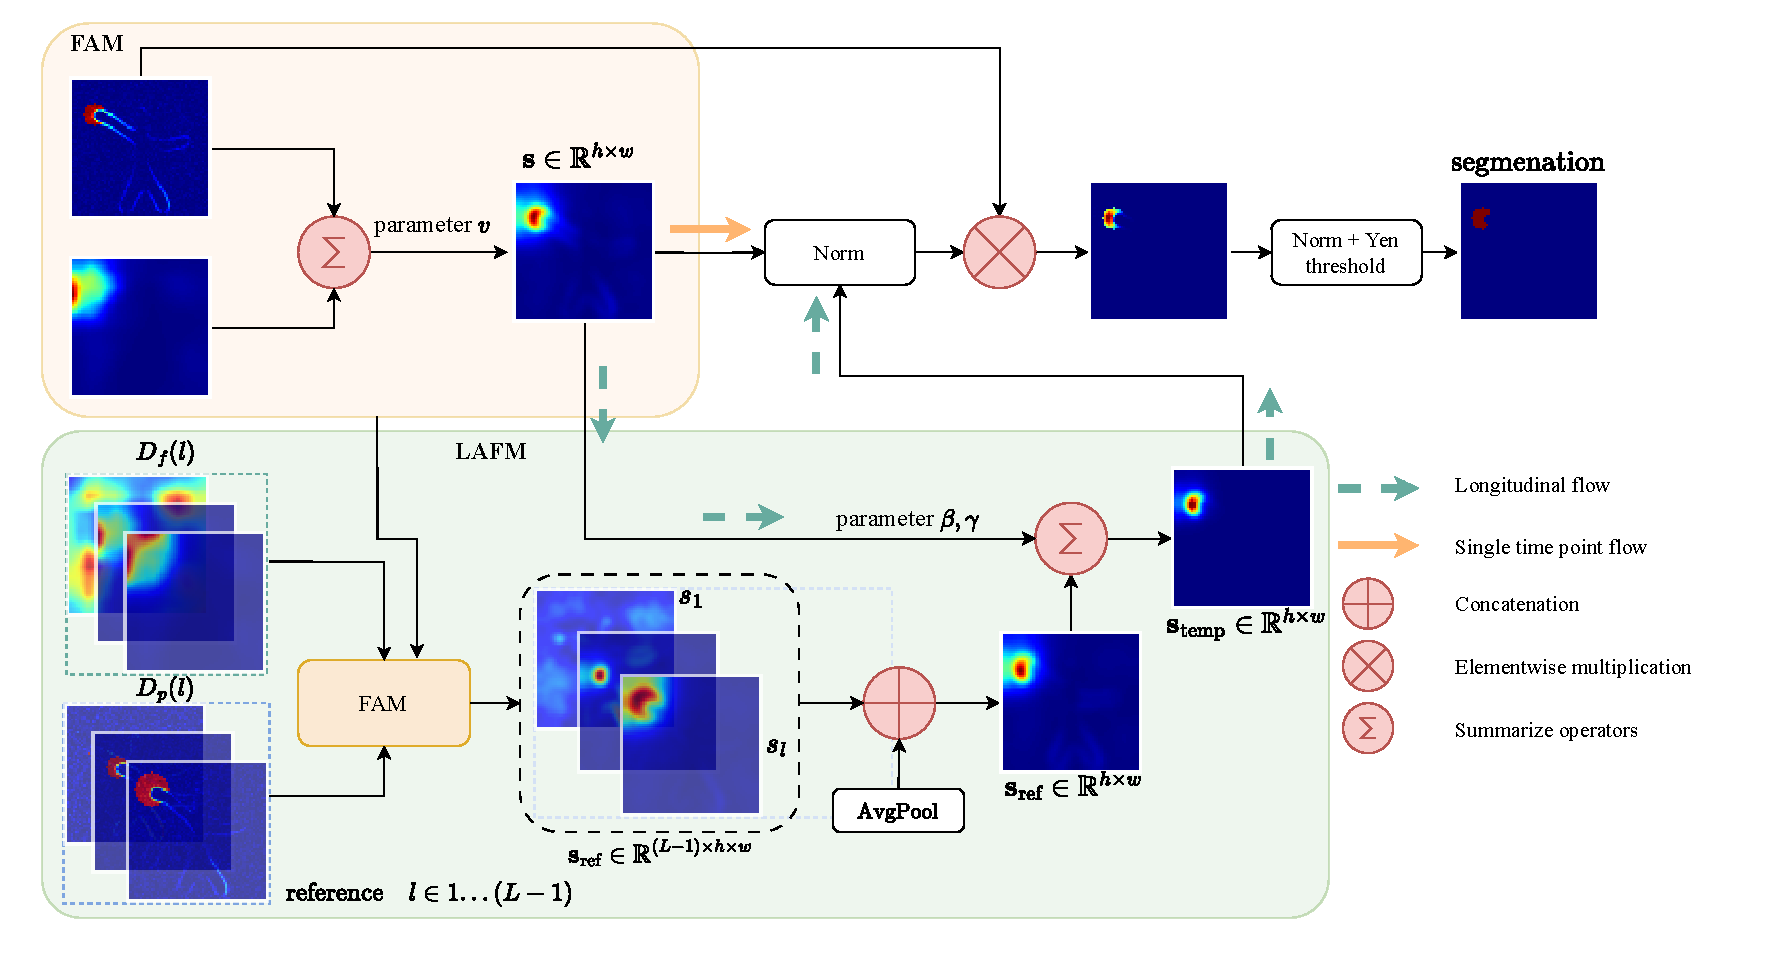
\includegraphics[width=0.95\linewidth]{figures/model-fam-lafm.pdf}
    \caption[Overview of FAM and LAFM module]{The overall structure of Feature Attention Module and Longitudinal Attention Fusion Module. For single time point (\textcolor{orange}{orange arrow}), anomaly segmentation is calculated directly from the output of FAM. With longitudinal data (\textcolor{green}{green arrow}), each time point anomaly score map is processed by FAM, concatenated together and applied the $F_{\text{mean}}$ operator with Gaussian weights (\cref{eq:laf_fusion}). The referenced anomaly score map $\rvx_{\text{ref}}$ is used to update the targeted anomaly score to have $\rvs_{\text{temp}}$ (\cref{eq:temp-smooth})}. 
    \label{fig:model-fam-lafm}
\end{figure}

Up to now, we have considered each sample as an i.i.d. draw from $p(\rvx)$. After combining feature distances and pixel distances from \cref{sec:feature-extractor-network}, each image $\rvx_0$ is associated with an anomaly score map $\rvs^{pixel} \in \mathbb{R}^{h \times w}$ that ideally contains sufficient information to determine which pixels are anomalous. Unfortunately, this is often not the case: if we detect anomalies independently at each time point, the anomaly score map can be noisy and exhibit: (i) false positives that appear at one time and then vanish, and (ii) missing of real anomalies (false negatives), especially when the anomalies are subtle. We assume that, in reality, anomalies usually have temporal persistence: they do not appear and disappear randomly\footnote{This might not be the case for patients undergoing treatment, but this scenario requires a different type of model and is beyond the scope of our experiment.}. Similar to \cite{wangEPDiffErasurePerception2025}, we design our \ac{LAFM} that acts as a temporal filter, enforcing the persistence of anomalies and smoothing out noise. We note that, in principle, our \ac{LAF} module is similar to the MAF module in \cite{wangEPDiffErasurePerception2025}, but instead of attending to information from multiple modalities at the same time point, here we concatenate information from a single modality across different time points. \cref{fig:model-fam-lafm} shows the overall structure of LAFM. 

We consider the full set of images collected for each patient, 
\[
\mathbf{X}_i = \{\rvx_1, \rvx_2, \dots, \rvx_L\}, \quad \rvx_l \in \mathbb{R}^{h \times w}, \quad l \in [1, \dots, L],
\] 
where $\rvx_l$ represents an image at a single time point $l$. Different patients may have a different total number of visits and images acquired at different time points. All images in the set $\mathbf{X}_i$ are processed through our \ac{SDM} model and \ac{FAM} as described above, yielding a corresponding set of anomaly score maps, 
\[
\mathbf{S}_i = \{\rvs_1, \rvs_2, \dots, \rvs_L\}.
\] 
We denote $\rvx$ as the target image and $\rvs$ as its corresponding anomaly score map at target time point $l_{\textnormal{target}}$. We further define the reference set 
\[
\rvs_{\text{ref}} = \mathbf{S}_i \setminus \{\rvs\}
\] 
as the set of anomaly score maps from other time points, excluding the target. Note that the length of $\rvs_{\text{ref}}$ is $L - 1$, and $\rvs_{\text{ref}} \in \mathbb{R}^{(L-1) \times h \times w}$.

Similar to MAF from \cite{wangEPDiffErasurePerception2025}, the role of \ac{LAFM} is to perform the weighted fusion of complementary information from reference time points, and ultimately to obtain the accurate anomaly masks. To fuse key information across time points and align it into a single output, we apply pixel-wise average pooling with a receptive field of 1. This gives us our mean response map $F_{mean}$ To account for the relative importance of each reference time point with respect to the target time point, we weight the reference anomaly score maps using a Gaussian kernel. Formally, we have: 

% We first concatenate all $\mathbf{S}_{\textnormal{ref}}$ together to obtain $\rvs_{\textnormal{ref}} \in \mathbb{R}^{(L-1) \times h \times w}$. 

\begin{equation}
\label{eq:laf_fusion}
\begin{aligned}
    \rvs_{\text{ref}} &= \oplus \{\rvs_l\}, \quad l \in [1, \dots, L], \; l \neq l_{\text{target}} \\
    \rvw &= \exp\Bigg(-\frac{(\rvl - l_\text{target}\mathbf{I})^2}{2\sigma^2}\Bigg) \\
    F_{\text{mean}} &= \mathrm{AvgPool}(\rvs_{\text{ref}} \odot \rvw) \in \mathbb{R}^{h \times w} 
\end{aligned}
\end{equation}

where 
\begin{itemize}
    \item $\mathbf{l} = [\, l_1, l_2, \dots, l_L \,]^\top$ is the vector of reference time points.
    \item \(l_\text{target}\) is the target time point.  
    \item \(\mathbf{w} = [\, w_1, w_2, \dots, w_L \,]^\top\) is the vector of Gaussian weights. 
    \item \(\sigma\) controls the temporal decay rate.
    \item $\oplus$ denotes concatenation and $\odot$ denotes element wise multiplication. 
\end{itemize}

Finally, we combine $\rvs_{\textnormal{ref}}$ with target anomaly score $\rvs$ using: 
\begin{align}
    \rvs_{\text{temp}} &= \underbrace{\rvs \times (1 - \beta \times (1 - \mathrm{Norm}(\rvs_{\text{ref}})))}_{\text{eliminate false positive}} + \underbrace{\gamma \times \rvs_{\text{ref}}}_{\text{eliminate false negative}} \label{eq:temp-smooth}
\end{align}

We refer to this as \emph{temporal smoothing operation} of $\rvs$, and it can be interpreted as follows: first, we normalize $\rvs_{\text{ref}}$ using min-max normalization. This transforms raw anomaly score into the scaled anomaly probability at each pixel. The first expression of RHS of \cref{eq:temp-smooth} is to eliminate false negative in target image. For example, if pixel $p_{i, j}$ is flagged as anomalous in $\rvs$, we check to see if it is consistent over time period. If this is a false positive, meaning this is pixel error cause by reconstruction process, it will not persist over time and thus its reference value across time will be small, i.e. $p_{i, j}^{\text{ref}, \text{norm}} \approx 0$. We negate its value and subtract it from $\rvs$, efficiently reducing its anomaly score. We note that here we are working with normalized scaled anomaly score $(1 - \mathrm{Norm}(\rvs_{\text{ref}})) \in [0, 1]$, so the target score will be scaled down according to its reference. Conversely, if the error persists over time, its reference value will be higher $p_{i, j}^{\text{ref}, \text{norm}} \approx 1$, and in this case we keep it unchanged. $\beta \in [0, 1]$ is hyperparameter controls how much the reference information influences the final anomaly score. In our setting, we choose $\beta = 1$ to strictly limit false positive, because in our experiments we observed that our model performs well in detecting anomalies, but tends to produce false positives on small pixel errors in healthy data. The second expression on the RHS of \cref{eq:temp-smooth} helps to decrease false negative. In particular, if a pixel $p_{i, j}^{\text{ref}, \text{norm}}$ is consistently flagged as anomalous across reference time points, but our model is false to detect in the current anomaly score map $\rvs$, we want to increase its value $p_{i, j}$. Hyperparameter $\gamma$ controls how much information is incorporated from $\rvs_{\text{ref}}$ to $\rvs$. As note earlier, false negatives are not a major issue in our model, so we set a relatively small $\gamma = 0.1$ as a safeguard mechanism. 

\subsection{Post Processing}
\label{sec:post-process}
\begin{description}
    \item[Pixel anomaly score]: We adapt some common post-processing technique used in UAD domain to further clean the residual map $\rvs_{l}$ before binarizing it to obtain anomaly segmentation \cite{behrendt2025cDDPM, baur_autoencoders_2020}. First, we apply a median filter with kernel size $k_{mf} = 5 \times 5$ to smooth out the anomaly score map, and to reduce the influence of noise to obtain a more reliable distribution of the anomalies. Next, we apply min–max normalization on a per-patient basis. This differs from other methods (cDDPM \cite{behrendt2025cDDPM}, EPDiff \cite{wangEPDiffErasurePerception2025}) where the authors apply normalization at each image/volume individually. 
    % By grouping all images from a single patient and performing the operation jointly, we provide more informatioachieve a more accurate separation between anomalous and healthy pixels. 
    \item[Pixel anomaly segmentation]: To obtain the localization of anomalies, a binary map is obtained by thresholding the anomaly score map. In previous methods \cite{autoDDPM, behrendt2025cDDPM, DDAD}, the optimal threshold for segmentation was found using a greedy search strategy on the validation dataset, by calculating the AUPRC metric and find the best theoretical value. However, ground truth annotations need to be provided in order to perform these search, and we argue that using labeled data will compromise the unsupervised setup (\cref{sec:introduction-sdm}). We follow \cite{wangEPDiffErasurePerception2025} to employ Yen threshold technique \cite{YenThreshold}, which is an automatic image thresholding strategy that can separate background and foreground based on histogram of gray levels in the image. We can formulate our whole post-processing for pixel anomaly score as follows: 
    \begin{equation}
    \label{eq:post-process-pixel}
        \begin{aligned}
            \mathbf{S}_{\text{temp}} &= [\rvs_{\text{temp},1}, \rvs_{\text{temp},2}, \dots, \rvs_{\text{temp},L}] \\
            \mathbf{S}_{\text{temp}} &= \mathrm{Norm} (\mathrm{MedianFilter}(k_{mf})(\mathbf{S}_{\text{temp}})) \\
            \text{thres} &= \mathrm{YenThreshold}(\mathbf{S}) \\
            \text{m}_{i, j} &= 
            \begin{cases}
            0 & \text{if } s_{i,j} < \text{thres} \\
            1 & \text{if } s_{i,j} \geq \text{thres}
            \end{cases} \\
            \mathbf{D}_{p} &= \text{m} \odot \mathbf{D}_p \\
            \text{p\_thres} &= \mathrm{YenThreshold}(\mathbf{D}_p) \\
            \text{p\_m}_{i,j} &=
            \begin{cases}
            0 & \text{if } d_{i,j} < \text{p\_thres} \\
            1 & \text{otherwise}
            \end{cases} \\
            \text{ano\_m} &= \text{m} \cap \text{p\_m}
        \end{aligned}
    \end{equation}

    where $\mathbf{S} \in \mathbb{R}^{L \times h \times w}$ is batch of all anomaly score maps (updated from LAFM) for 1 patient $i$, and $\mathbf{D}_p \in \mathbb{R}^{L \times h \times w}$ is batch of all pixel distance maps. Here we drop the subscript $i$ for brevity. $\text{m}$ and $\text{p\_m}$ are anomaly score segmentation maps and pixel distance segmentation maps, respectively. The final anomaly segmentation maps are defined as intersection between the twos. 
    
    \item[Image anomaly score]: After post-processing step, we obtain the pixel-level anomaly score $\rvs \in \mathbb{R}^{h \times w}$ for each individual image. For image-level anomaly score, a common practice in the literature is taking the mean over all pixel values in the anomaly map. \cite{DDAD, lagogiannisUnsupervisedPathologyDetection2024} use the maximum value across pixels and assign it as the overall anomaly score of the image, with the argument that it should be independent of the anomaly size. \cite{wuUADPostSampling2024} combine both technique and design the image-wise anomaly score as the average of the largest $S$ pixel wise anomaly scores in $\rvs$ to mitigate false positives caused by image noise. We employ several similar techniques, which will be discussed in \cref{sec:image-auprc-auroc}.
\end{description}



% There are some common post-processing technique irst, we apply a median filter with kernal size of $K = 5 \times 5 \times 5$ to smooth the residual map. Next, we perform barin mask eroding for 3 iterations to filter out pixel differences caused by poor reconstructions along the sharp edge of the object. Finally, the binary segmentation map $\rvm \in \sR^{h \times w}$ is obtained by thresholding the post-processed residual map $\rvr \in \sR^{h \times w}$, using $m_{i, j} = 1$ if $\rvr_{i,j} > \mathrm{threshold}$, otherwise $m_{i, j} = $. As a final step, following the method of \cite{behrendt2025cDDPM}, we use connected component filtering to remove areas that include less than 7 voxels. In this step, we can make use of domain-specific knowledge to further remove false-positive predictions that are smaller than the anomalies considered in our study.  

% \subsubsubsection{Some other post-processing technique}

% \begin{description}
%     \item[\href{https://hal.science/hal-02995591/file/Papier_MEDIA_Alaverdyan_2020.pdf}{Regularized siamese autoencoder for UAD in MRI}]: 3 steps techniques that first normalizing the distance maps with respect to the intra-subject spatial variability. For that purpose, the distance maps of the control subjects are computed by performing a k-fold evaluation of the training set (i.e. for each fold of normal subjects, the distance maps are obtained with oc-SVMs trained on the remaining subjects). The second step is to pool all pixel-wise distance into a histogram and estimate the distribution with non-parametric method (kernel density estimation). 26 connectivity then used to define cluster. Finally, the third step consists in ranking the cluster. 

%     \item[\href{https://hal.science/hal-03962874v1/document}{Voxel based OC-SVM}]: perform Oc-SVM at each pixel/voxel, i.e each voxel will fit 1 OC-SVM model. Each voxel is represented by a feature vector $\mathbf{V}^d$ with ($d=2$), so OC-SVM is trained with $n$ vector of 2 dimensional. Given a test sample we will obtain a OC-SVM distance map by trained OC-SVM models for each voxel, we will use the raw score as OCSVM map. thresholding this score map is done by modeling the probability distribution of the OC-SVM scores for normal voxel. This normative score distribution was computed by performing a leave-one-out procedure on the normal subjects (or we can use $k-$fold strategy). Assuming we obtain $k$ score map (on healthy training dataset), $k$ corresponding histograms are calculate with the same bin width and value range, normative histogram is obtained by averaging all $k$ histogram. This distribution was then approximated by a non-parametric distribution using a kernel density estimator to convert score values into probability density estimates. We assume that the OC-SVM score distribution of any given test patient can be represented by this normative score distribution, except those are inside anomaly region which we can consider to be outlier of the distribution. The type I error can then be controlled by using a threshold value that corresponds to a given $p-$value on the normative distribution. 
%     The clustering process then consists in scanning the thresholded map in a lexico-graphical voxel order and aggregating all non-null voxels that are linked for the 26-connectivity rule. Descriptive statistics per cluster (size, minimum, maximum and mean of the voxel scores) are then computed. Each cluster is assigned a value that corresponds to the minimum OC-SVM score value of its constituting voxels, i.e. the smallest probability value of belonging to the normal class. Finally, a labelled cluster map is generated in which cluster order is given by the minimum (i.e. most pathological) OC-SVM score value.
% \end{description}

% \subsubsection{Pixel anomaly score and Image anomaly score}

% After post-processing step, we obtain the pixel-level anomaly score $\rvr \in \sR^{h \times w}$. For image-level anomaly score, a common practice in the literature is taking the mean over all pixel values in the anomaly map. \cite{DDAD, lagogiannisUnsupervisedPathologyDetection2024} use the maximum value across pixels and assign it as the overall anomaly score of the image, with the argument that it should be independent of the anomaly size. \cite{wuUADPostSampling2024} combine both technique and design the image-wise anomaly score as the average of the largest $S$ pixel wise anomaly scores in $\rvr$ to mitigate false positives caused by image noise. 

% \subsubsection{Anomaly threshold}

% In the field of UAD for medical images, selecting an appropriate threshold remains a critical and ongoing challenge—both for binarizing the anomaly score map to obtain pixel-level anomaly segmentation, and for assigning a single class label at the image level. 

% \subsection{One Class SVM}

% Reference from paper: \href{https://hal.science/hal-05164029/document}{OVSVM guided autoencoder for UAD}
% \\
% The dual form of OCSVM is as follow: 
% \begin{align}
%     \min_{\alpha} \frac{1}{2} \sum_{i=1}^{n}\sum_{j=1}^{n} \alpha_i \alpha_j k(\rvz_i, \rvz_j) \\
%     \text{subject to: } 0 \leq \alpha \leq \frac{1}{\nu n} \quad n \in [1, n] \notag \\
%     \sum\alpha_i = 1 \notag
% \end{align}

% OCSVM is solved using \texttt{cvxpy} package, in which we optimize over $\alpha^*$ with fixed kernel $K$. However, in the coupled setting we integrate our function into our neural network, and $K$ depends on the latent variable $\rvz_i$. The optimization problem ( \verb+CvxpyLayer+) solves for $\alpha$, but the loss depends on how the features $\rvx_i$ produce a good decision boundary.
% Backpropagation flows through the solution of the \verb+CVXPY+ problem (through the optimzed $\alpha*$ values), back to the parameters $\theta$ of our network. For this reason, we indirectly optimize $K$ using OCSVM. 

% \verb+CVXPY+ must recognize the problem as \emph{disciplined convex programming} (DCP) compliant, and we cannot have parameters appear in quadratic form. We utilize the fact that $K$ is positive semi-definite (a gram matrix) to rewrite the problem as: 
% \begin{align}
%     K &= K^{\frac{1}{2}T} K^{\frac{1}{2}} \\
%     \bm{\alpha}^TK \bm\alpha &= \bm\alpha^T K^{\frac{1}{2}T} K^{\frac{1}{2}} \bm\alpha \\
%     \bm{\alpha}^TK \bm\alpha &= \|K^{\frac{1}{2}}\bm\alpha\|^2
% \end{align}

% \subsubsection{OCSVM for Image-wise anomaly score}

% We will train our OCSVM model on semantic encoder output $\rvy_{\text{sem}} = \mathrm{Enc_{\phi}(\rvx)}$, based on the assumption that after diffusion training, $\rvy_{\text{sem}}$ captures the most important features of our input and can be use to generate new sample that shares the same structure as input. We also utilize OCSVM step to further reduce the dimension of $\rvy_{\text{sem}}$ for downstream task of longitudinal learning, thus we include a small autoencoder network in OCSVM $\rvz_{\text{sem}} = \mathcal{E}(\rvy_{\text{sem}})$ and OCSVM will learn the decision boundary on these latent variabls instead of directly on $\rvy_{\text{sem}}$. To minimize the underlying rank of $\rvz_{\text{sem}}$, we follow the method of \href{https://arxiv.org/abs/2010.00679}{implicit rank-minizing autoencoder} by adding $l$ linear transformation matrices between encoder and decoder. The latent variable $\rvz_{\text{sem}}$ becomes: 

% \begin{equation}
%     \rvz_{\text{sem}} = \mathcal{D}(W_l \dots W_2 W_1 \mathcal{E}(\rvy_{\text{sem}}))
% \end{equation}

% \textbf{Main idea of the paper}: a series of linear matrices $W_l \dots W_2 W_1$ form a linear neural network between the encoder and decoder, acting as an implicit regularization. During training, these matrices encourage latent variables to use a lower number of dimensions and effectively minimize the rank of covariance matrix of the latent space. Each $W_i \quad i \in [1 \dots L]$ is a square matrix that does not change the dimension between input and output. We note that these matrices are equivalent to a single linear layer at inference time, and thus they do not change the capacity of the autoencoder. 

% IRMAE \href{https://github.com/facebookresearch/irmae/blob/main/model.py}{github}



\chapter{Experiment}
\label{chap:experiment}
\minitoc

\section{Dataset}
\label{sec:dataset}

% \subsubsection{Synthetic Starmen dataset}

We use the \texttt{Starmen} dataset as a toy example to test and demonstrate the performance of our model. The \texttt{Starmen} dataset is a synthetic longitudinal dataset\footnote{The dataset is available at \href{https://zenodo.org/records/5081988}{https://zenodo.org/records/5081988}} consisting of $N = 1,000$ subject, each with $10$ visits at different time points. This dataset is specifically designed for studying longitudinal models, capturing both spatial and temporal variability. The temporal variability of the population is prescribed by a "starman" raising its left arm, generated according to a diffeomorphism model described in \cite{bôneStarmenDataset2018}. On the other hand, the spatial variability represents individual heterogeneity are characterized by the location of other four control points: the head, right arm and legs. This way, the effects of time progression, raising the left arm, are (spatially) independent of the inter-variability of the shapes. All subjects raise the left arm but vary in shape with different position of their legs and arms.

All images are gray scaled with 1 channel $(1 \times 64 \times 64)$, and pixel values are normalized in the range $[0, 1]$. We use $700$ patients for our training set, $150$ for validation set and $150$ for test set. We note that 1 patient has 10 visits, thus when we consider individual images we have $7000, 1500$ and $1500$ samples for train, validation and test set, respectively. We consider all images in these sets are healthy. Since this dataset does not have anomaly structure, we use \texttt{cv2} package to generate 3 types of synthetic anomaly to be used in our anomaly detection task: \texttt{growing\_circle}, \texttt{darker\_line} and \texttt{darker\_circle}. For each type of anomaly, we create an anomaly set of $20$ patients, corresponding to $200$ anomaly images. \cref{fig:example_starmen} shows 1 example of healthy patient and 3 synthetic anomaly types.

\begin{figure}
    \centering
    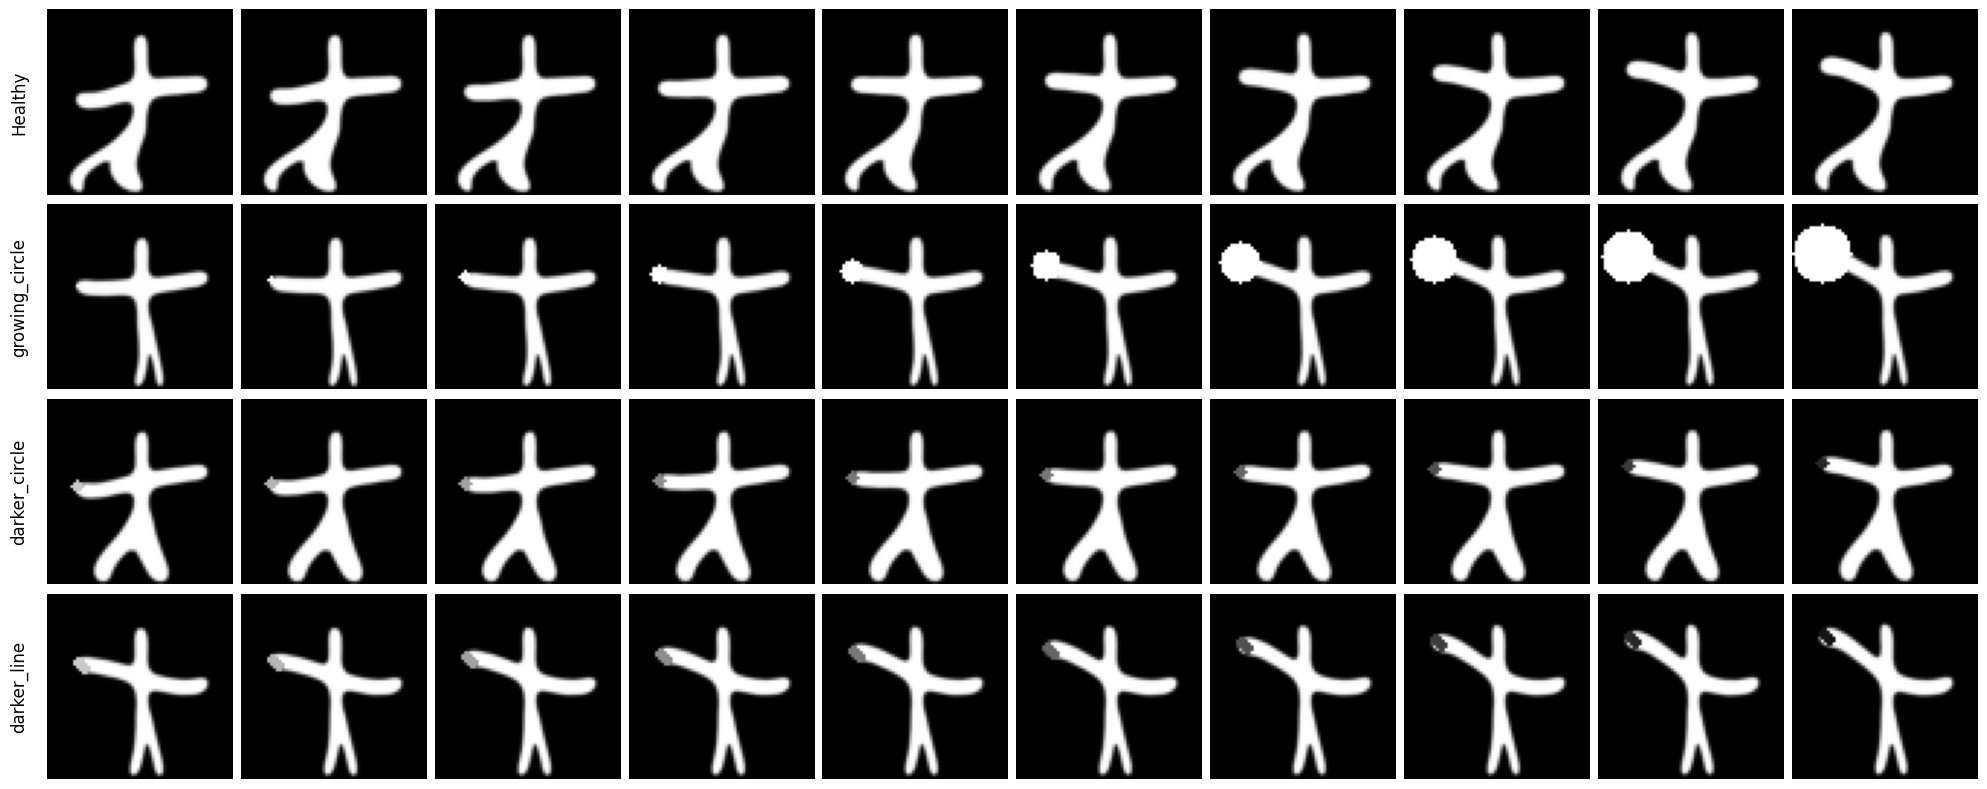
\includegraphics[width=0.75\linewidth]{figures/example_starmen.png}
    \caption[Example of \texttt{Starmen} dataset]{Examples of Starmen dataset images. The first row shows a healthy image. The last 3 rows show different anomaly type, from top to bottom: anomaly of type \texttt{growing\_circle}, anomaly of type \texttt{darker\_circle} and \texttt{darker\_line}. Each sample contains 10 sequential images at different time points, through time the mini starmen slowly raises its left hand, while maintaining all other parts of its body (head, legs and right hand). Anomalies are added using \texttt{cv2} and places at the left most points of the figure.}
    \label{fig:example_starmen}
\end{figure}

% Synthetic longitudinal dataset of starmen images  (64x64), based on the longitudinal diffeomorphic model. The cross-sectional variability of the population is prescribed by a diffeomorphism localized at four control points: the head, right arm and legs. The common progression timeline, on the other hand, is generated through a displacement of the left arm only.
% This way, the effects of time progression, raising the left arm, are (spatially) independent from the inter-variability of the shapes. All subjects raise the left arm but vary in shape with different position of their legs and arms. The dataset is comprised of $N=1000$ objects, each with $10$ visit at different time points. 

% The dynamics of progression is given by an affine reparametrization of the age at the visit, characterized by individual onset and acceleration factors, such that the true progression of the disease is given by. 

% The dataset description is given in \verb|df.csv| files, with columns: 

% \begin{itemize}
%     \item \texttt{tau}:  the onset age - the age at which a disease starts or a developmental process begins.
    
%     \item \texttt{t}: the actual age or observation time point.
    
%     \item \texttt{path}: absolute path to the subject gray scale image (1x64x64). The image is generated from `vtk` file. 
    
%     \item \texttt{id}: subject ID

%     \item \texttt{alpha}: the acceleration factor - how fast a disease developes. 
    
% \end{itemize}

% \subsubsection{Some useful github repos to process - visualize the dataset}

% \begin{itemize}
%     \item \href{https://github.com/MChen808/UOMETM/tree/main}{UOMETM repo}

% \end{itemize}

\section{Implementation details}
\label{sec:implementation}

\subsection{Spatial Diffusion Model}

\paragraph{UNet}: The baseline diffusion model is based on the DDIM model \cite{songDDIM}\footnote{Available at \href{https://github.com/openai/guideddiffusion}{https://github.com/openai/guideddiffusion}} with adaptation from LDAE \cite{lozuponeLDAE2025} \footnote{Available at \href{https://github.com/GabrieleLozupone/LDAE}{https://github.com/GabrieleLozupone/LDAE}}. The UNet comprises an input block, a middle block and an output block. The input block follows an encoder architecture that encodes and downsamples the original input. The output blocks are symmetric counterparts of the encoder, upsampling the encoded representation back to the original resolution. Each block contains one residual block (ResBlock), with channel multipliers of $[32, 64, 96]$. Each ResBlock begins with a GroupNorm layer and a SiLU activation, followed by a Conv2d layer with kernel size $(3, 3)$ and stride $(1, 1)$. Downsampling is performed with an AvgPool layer of kernel size $(2, 2)$, stride $(2, 2)$, and no padding. Attention layers are added at resolution scales of $[\tfrac{1}{2}, \tfrac{1}{4}]$ to capture dependencies across neighboring regions of the image and enhance spatial information exchange between feature maps. 
\paragraph{Condition signals}: time step condition $t$ is embedded using sinusoidal time step embeddings, originated from \cite{vaswani2023attentionneed}. The embedded $t$ is then projected through a linear layer followed by a SiLU activation to obtain a vector of dimension $d_{cond} = 128$. We use ResNet50 as the backbone for the semantic encoder $\mathrm{Enc}{\phi}$. The parameters $\phi$ are initialized from the pretrained ResNet module in PyTorch. The final classifier layer of ResNet is replaced with a fully connected layer to produce a non-spatial representation of the input, $\rvy_{sem} = \mathrm{Enc}_{\phi}(\rvx)$, with latent dimension $d = 512$. This representation is further projected via linear layers to match the dimension of the time step embedding. Finally, the conditioning variables $(\rvy_{sem}, t)$ are injected into the network using AdaGN. 
\paragraph{Training configuration}: \ac{SDM} is trained with a total number of diffusion time steps $T = 1000$ and a linear noise variance from $\beta_1 = 0.0001$ to $\beta_T = 0.02$. We use the Adam optimizer with a learning rate of $2 \times 10^{-5}$. Training is performed for 500 epochs with a training batch size of $2$ patients, corresponding to an effective batch size of $20$ samples. Following common practice in diffusion models \cite{lozuponeLDAE2025, rombachLDM}, we use an exponential moving average (EMA) to stabilize training and improve generalization. EMA decay rate is $0.999$, and EMA parameters are updated after every 10 batches. A full list of architectural and training parameters is provided in \cref{tab:sdm-config}.

\begin{table}[h]
\captionsetup{justification=raggedright,singlelinecheck=false}
\caption{Spatial Diffusion Model (SDM): configurations and parameters}
% \resizebox{\columnwidth}{!}{%

\begin{adjustbox}{max width=0.9\textwidth}
    \begin{tabular}{ll}
    \toprule
    \multicolumn{2}{l}{\textbf{Semantic Encoder $\mathrm{Enc}_{\phi}$}} \\
    \midrule
    Backbone & \texttt{ResNet50}\cite{ResNet50} \\
    Pretrained Init & ImageNet \\
    Input Modality & $1 \times 64 \times 64 $ \\
    Output layer & \texttt{Linear(in=1000, out=512)} \\
    Output Representation & non-spatial vector $\mathbf{y}_{sem} \in \mathbb{R}^{512}$ \\
    \midrule
    \multicolumn{2}{l}{\textbf{Diffusion UNet $\epsilon_{\theta}$}} \\
    \midrule
    Input Shape & $(\text{B}, 1, 64, 64)$, with batch size first \\
    Channels multipliers & [32, 64, 96] \\
    Residual Blocks per Level & 1 \\
    Attention Resolutions (factors) & [2, 4] \\
    Number of attention head & 1 \\
    Conditional injection & AdaGN (scale-shift norm) \\
    Dropout & 0.1 \\
    Time embedded dimension & $d_{cond} = 128$ \\
    Semantic encoder dimension & $d_{sem}=512$ \\
    Timestep & 1000 \\
    Beta Schedule & Linear, $\beta_t \in [10^{-4}, 2 \times 10^{-2}]$ \\
    \midrule
    \multicolumn{2}{l}{\textbf{Training Configuration}} \\
    \midrule
    Optimizer & Adam \\
    Learning Rate & $2.5 \times 10^{-5}$ \\
    EMA Decay & 0.999 \\
    Train Batch Size (effective) & 20 \\
    Training Duration & 500 epochs / $\sim$3 hours \\
    Hardware & 2 x Nvidia L40S (45 GiB) \\
    \bottomrule
    \end{tabular}
\end{adjustbox}
% }
\label{tab:sdm-config}
\end{table}

\subsection{Feature Extractor network of FAM}

Our FE network $\Phi$ is initialized from trained semantic encoder $\mathrm{Enc}_{\phi}$. To learn the similarity between samples, each training batch $\rvx \in \mathbb{R}^{B \times 1 \times 64 \times 64}$ is passed through the SDM model to obtain its reconstruction $\widehat{\rvx} \in \mathbb{R}^{B \times 1 \times 64 \times 64}$. We employ the DDIM sampling scheme in the denoising process with 100 steps to accelerate training. To improve generalization, we reconstruct $\rvx$ from different noise levels $[100, 250, 500, 1000]$, selected uniformly at each epoch. Cosine similarity loss is calculated on three layers of ResNet50, each at a different resolution, and the losses are summed to obtain the total loss. Distillation loss is incorporated from frozen $\mathrm{Enc}_{\phi}$ network, with parameter $\lambda_{DL} = 1$, using \cref{eq:fe-dl-loss}. FE is trained with 100 epochs, using Adam optimizer with learning rate $10^{-4}$. \cref{tab:fe-config} shows the details configurations of our FE network.  

\begin{table}[h]
\captionsetup{justification=raggedright,singlelinecheck=false}
\caption{Feature Extractor network (FE): configurations and parameters}
% \resizebox{\columnwidth}{!}{%
\begin{tabular}{ll}
\toprule
\multicolumn{2}{l}{\textbf{FE $\Phi$}} \\
\midrule
Backbone & \texttt{ResNet50}\cite{ResNet50} \\
Pretrained Init & Semantic Encoder $\mathrm{Enc}_{\phi}$ \\
Architecture & Same as $\mathrm{Enc}_{\phi}$ \\
Input Shape & $(B, 1, 64, 64)$, with leading dimension is batch size \\
Feature layers & [\texttt{layer1, layer2, layer3}] \\
Feature size - \texttt{layer1} & [256, 64, 64] \\
Feature size - \texttt{layer2} & [512, 8, 8] \\
Feature size - \texttt{layer3} & [1024, 4, 4] \\
DDIM samle step & 100 \\
Noise level & [100, 250, 500, 1000] \\
$\lambda_{DL}$ & 0.1 \\
Optimizer & Adam \\
Learning Rate & $1.0 \times 10^{-4}$ \\
Train Batch Size (effective) & 20 \\
Training Duration & 100 epochs / $\sim$4 hours \\
Hardware & 1 x Nvidia L40S (45 GiB) \\
\bottomrule
\end{tabular}
% }
\label{tab:fe-config}
\end{table}

\section{Evaluation metrics}

The performance of our model is evaluated based on two main criteria: reconstruction quality and anomaly detection score. In this section, we outline the details of our evaluation metrics for both tasks. 

\subsection{Reconstruction quality}

For both SDM and TDM, the goal of diffusion model is to reconstruct the ground truth image: it can be the original healthy image (in the case of SDM), or the ground truth missing image (in the case of TDM). To evaluate the overall reconstruction quality, we follow conventional methods in literature \cite{rombachLDM, lozuponeLDAE2025, behrendt2025cDDPM}, and calculate both pixel error metrics and similarity metrics between inputs and reconstructed images. For pixel error, we report both the $l1$ and $l2$ errors. For similarity, we consider the Structural Similarity Index Measure (SSIM), the Peak Signal To Noise Ratio (PSNR) and the Learned Perceptual Image Patch Similarity (LPIPS) as metrics to assess the reconstruction quality. To account for perceptual structures at both coarse scales and fine details scales, we also calculate the Multi Scale Structural Similarity (MSSIM), which is more aligned with human visual perception. For the feature based LPIPs metric, features are extracted by a \texttt{squeeze} network. All similarity metrics are implemented in \texttt{Monai} package \footnote{MONAI is an open-source framework for deep learning in healthcare imaging, available at \href{https://docs.monai.io/en/stable/index.html}{https://docs.monai.io/en/stable/index.html}}. 

Furthermore, for anomaly detection task, only healthy anatomy should be reconstructed. Similar to \cite{behrendt2025cDDPM}, we consider the $l1$-error of healthy and unhealthy anatomy separately, given the synthetic anomaly data sets. Specifically, we calculate the $l1$-error for both healthy and unhealthy anatomy, as indicated by the annotation masks and also calculate an $l1$-ratio as follows:
\begin{equation}
    l1\text{-ratio} = \frac{l1_{anomaly}}{l1_{healthy}}
    \label{eq:l1-ratio}
\end{equation}

For healthy region, we want to have as small error as possible, while for anomaly region it is better to have higher errors, which will help to separate anomaly part from healthy structure. A higher value for $l1$-ratio indicates that the model successfully remove the anomaly region while maintaining correct structure of healthy anatomy, and vice versa. 

\subsection{Anomaly scores}

To evaluate the performance of our models in anomaly detection, we use the ground-truth segmentation from our synthetic anomaly dataset. It is important to note that ground-truth labels/annotations are often unavailable in real-life MRI datasets, especially in unsupervised settings. Nevertheless, most common models still rely on datasets with ground-truth labels to assess their performance, as reported in Bercea’s study \cite{berceaDDPMforMedicalImagesStudy2024}.

\textbf{Image-level anomaly detection}: recall from \cref{sec:post-process} that from a spatial anomaly score map, we use several functions to summarize all pixel-level score into 1 single value that we can assign for image level anomaly score. The AUROC and AUPRC are popular metrics \cite{wu2024maskdiffusionposteriorMDPS, behrendt2025cDDPM, DDAD, wangEPDiffErasurePerception2025} due to their threshold independence, so we can assess the model's performance directly from raw anomaly score without having to find a threshold value. However, AUROC is reported to have potential misleading in imbalanced datasets dominated by the majority class \cite{berceaDDPMforMedicalImagesStudy2024}. The AUPRC focuses on precision recall trade-offs and offers better evaluations in imbalanced datasets where anomalies are scarce. 

\textbf{Pixel-level anomaly localization}: at pixel level, we care about the segmentation of anomaly. Following \cite{behrendt2025cDDPM, wangEPDiffErasurePerception2025}, we use the Dice score metric, which measures the overlap between the predicted and ground truth segmentations, providing a single value that balances false positives and false negatives \cite{berceaDDPMforMedicalImagesStudy2024}. The Dice score is given by: 

\begin{equation}
    \label{eq:dice-score}
    \mathrm{DICE} = \frac{2. |A \cap B|}{|A| + |B|}
\end{equation}

where $A$ and $B$ are the anomaly map and the ground truth segmentation, respectively. One disadvantage of this metric is that it requires setting a threshold value from our anomaly score maps to determine whether a pixel is classified as anomalous, which can significantly impact results. As mentioned in \cref{sec:post-process}, we will use Yen threshold technique, which can provide automatic threshold value without using any greedy search algorithm.  

\chapter{Results}
\label{chap:result}

\minitoc 

\section{Reconstruction with SDM}
\label{sec:result-sdm}

\subsection{Reconstruction quality}
\label{sec:result-reconstruction-error}

\begin{figure}
    \centering
    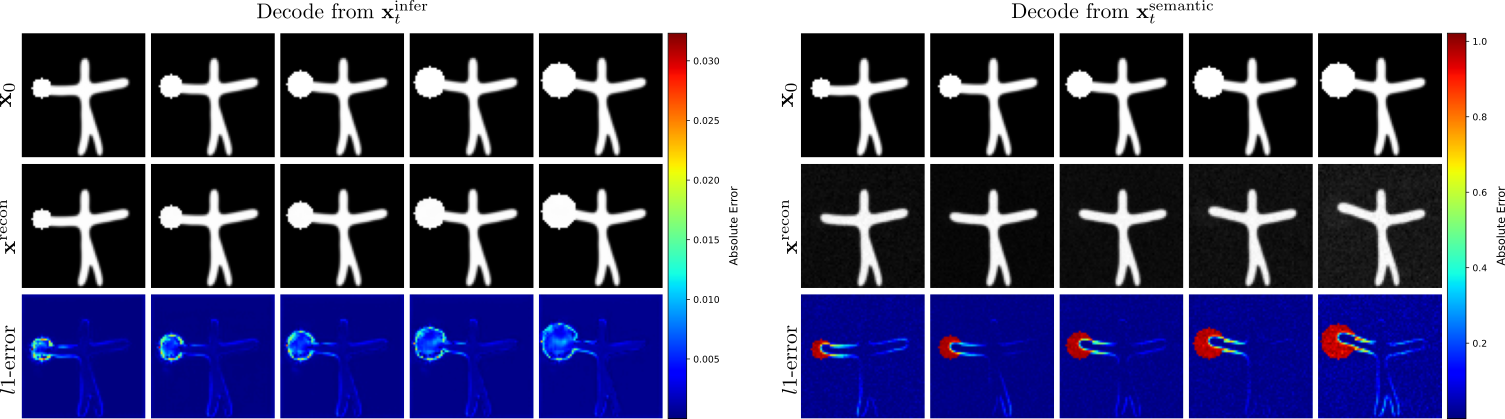
\includegraphics[width=0.75\linewidth]{figures/compare-effect-infer.png}
    \caption[Reconstructions from random noise and from stochastic subcode]{Reconstruction error when decoding from $\rvx_T^{\text{infer}}$ (left) and $\rvx_T^{\text{semantic}}$ (right). From top to bottom: the original image, the reconstructed image and residual error. Note that the color code is not on the same scale for all images.}
    \label{fig:compare-effect-infer}
\end{figure}

\autoref{tab:error-starmen} presents the quantitative results of reconstruction errors for two experiments: denoising from pure random noise and denoising from a stochastic subcode of the input $\rvx$. The term \texttt{semantic} indicates that $\rvx_T$ is obtained by adding random Gaussian noise, whereas \texttt{infer} refers to $\rvx_T$ generated by applying the reversed DDIM process (stochastic encoding) to $\rvx$. All results are evaluated by first noising the image to a noise level of $250$, followed by denoising using the DDIM sampling scheme with 250 denoising steps. We observe that using $\rvx_T^{\text{infer}}$ yields much smaller reconstruction errors and significantly higher similarity metrics. This improvement arises because $\rvx_T^{\text{infer}}$ retains fine-grained details about the input, which are absent in the semantic encoding, and thus better guides the diffusion process toward the true distribution of the original image. For the healthy dataset and subtle anomaly types \texttt{darker\_line} and \texttt{darker\_circle}, we observe extreme cases where MSSIM reaches $100\%$, indicating that perceptually the reconstructed image is indistinguishable from the original to a human observer. On the other hand, this raises a problem of “anomaly preservation", which indicates that the anomaly region is preserved in the reconstructed image. We can see this in the $l_1$-ratio for \texttt{growing\_circle}: it is much higher when denoising from $\rvx_T^{\text{semantic}}$ compared to $\rvx_T^{\text{infer}}$, because the former completely removes the anomaly, whereas the latter preserves it via information encoded in the stochastic subcode. For the case of very subtle anomalies, $l1$-ratio is higher when denoising from $\rvx_T^{\text{infer}}$, this is because the $l_1$-error within the anomaly region is relatively small, which can be attributed to the subtlety of the anomaly. Nevertheless, we can still observe the perceptual effects of anomaly preservation, as well as the qualitative results of different types of reconstruction errors, in \cref{fig:compare-effect-infer}. 

\begin{table}[htbp]
\centering
\caption[Comparison of reconstruction quality]{Comparison of the reconstruction quality of different test datasets. \texttt{\textcolor{blue}{test\_healthy}} refers to healthy dataset, while others correspond to various anomaly types. Dataset name follows format \texttt{<dataset> ($N$)}, where $N$ indicates the number of patients (each patient has 10 longitudinal samples). For all metrics, the mean ± standard deviation across whole dataset are reported. The arrows $\uparrow$ and $\downarrow$ indicate that higher and lower values are favorable, respectively.}
\label{tab:error-starmen}

\begin{subtable}{\textwidth}
    \centering
    \begin{adjustbox}{max width=\textwidth}
    % \resizebox{0.95\textwidth}{!}{%
    \begin{tabular}{lrrrr}
    \toprule
     & \multicolumn{2}{r}{\texttt{\textcolor{blue}{test\_healthy}} (150)} & \multicolumn{2}{r}{\texttt{\textcolor{red}{growing\_circle}} (20)} \\
     & semantic & infer & semantic & infer \\
    \midrule
    $l1 \mathrm{-All}$ (e-3) $\downarrow$ & 12.61 ± 23.94 & 1.04 ± 1.97 & 32.79 ± 125.79 & 0.75 ± 2.07 \\
    $l1 \mathrm{-Anomaly}$ (e-3) $\uparrow$ & - & - & 743.48 ± 372.27 & 6.52 ± 6.44 \\
    $l1 \mathrm{-Healthy}$ (e-3) $\downarrow$ & - & - & 16.44 ± 33.34 & 0.62 ± 1.63 \\
    $l1 \mathrm{-ratio} \uparrow$ & - & - & 45.23 & 10.58 \\
    \cline{1-5}
    $l2 \mathrm{-All}$ (e-3) $\downarrow$ & 0.73 ± 8.26 & 0.00 ± 0.03 & 16.90 ± 118.55 & 0.00 ± 0.08 \\
    $l2 \mathrm{-Anomaly}$ (e-3) $\uparrow$ & - & - & 691.34 ± 388.77 & 0.08 ± 0.45 \\
    $l2 \mathrm{-Healthy}$ (e-3) $\downarrow$ & - & - & 1.38 ± 13.98 & 0.00 ± 0.04 \\
    \cline{1-5}
    $D_{f} \mathrm{-All}$ (e-3) $\downarrow$ & 2.48 ± 2.02 & 0.01 ± 0.01 & 31.50 ± 81.52 & 0.02 ± 0.05 \\
    $D_{f} \mathrm{-Anomaly}$ (e-3) $\uparrow$ & - & - & 306.74 ± 165.98 & 0.10 ± 0.08 \\
    $D_{f} \mathrm{-Healthy}$ (e-3) $\downarrow$ & - & - & 25.17 ± 66.19 & 0.02 ± 0.05 \\
    \cline{1-5}
    SSIM $\uparrow$ & 85.70 ± 5.12 & 99.89 ± 0.02 & 75.00 ± 14.64 & 99.86 ± 0.05 \\
    MSSIM $\uparrow$ & 98.85 ± 0.50 & 100.00 ± 0.00 & 93.76 ± 5.09 & 99.99 ± 0.00 \\
    PSNR $\uparrow$ & 32.66 ± 3.00 & 53.27 ± 1.32 & 21.19 ± 6.57 & 53.19 ± 0.66 \\
    \bottomrule
    \end{tabular}
    \end{adjustbox}
    % }
\label{tab:error-starmen-a}
\caption{Reconstruction metrics for healthy dataset and growing circle anomaly}
\end{subtable}

\vspace{0.5em}

\begin{subtable}{\textwidth}
    \centering
    % \resizebox{0.95\textwidth}{!}{%
    \begin{adjustbox}{max width=\textwidth}
    \begin{tabular}{lrrrr}
    \toprule
     & \multicolumn{2}{r}{\texttt{\textcolor{red}{darker\_line}} (20)} & \multicolumn{2}{r}{\texttt{\textcolor{red}{darker\_circle}} (20)} \\
     & semantic & infer & semantic & infer \\
    \midrule
    $l1 \mathrm{-All}$ (e-3) $\downarrow$ & 14.93 ± 42.74 & 0.47 ± 1.88 & 14.60 ± 37.13 & 0.59 ± 2.09 \\
    $l1 \mathrm{-Anomaly}$ (e-3) $\uparrow$ & 400.49 ± 240.64 & 14.48 ± 10.88 & 385.45 ± 230.77 & 19.93 ± 14.25 \\
    $l1 \mathrm{-Healthy}$ (e-3) $\downarrow$ & 13.06 ± 28.79 & 0.41 ± 1.42 & 13.50 ± 28.58 & 0.53 ± 1.64 \\
    $l1 \mathrm{-ratio} \uparrow$ & 30.66 & 35.64 & 28.56 & 37.65 \\
    \cline{1-5}
    $l2 \mathrm{-All}$ (e-3) $\downarrow$ & 2.05 ± 27.42 & 0.00 ± 0.05 & 1.59 ± 19.48 & 0.00 ± 0.08 \\
    $l2 \mathrm{-Anomaly}$ (e-3) $\uparrow$ & 218.28 ± 216.30 & 0.33 ± 0.46 & 201.81 ± 198.32 & 0.60 ± 0.93 \\
    $l2 \mathrm{-Healthy}$ (e-3) $\downarrow$ & 1.00 ± 17.33 & 0.00 ± 0.03 & 1.00 ± 12.06 & 0.00 ± 0.05 \\
    \cline{1-5}
    $D_{f} \mathrm{-All}$ (e-3) $\downarrow$ & 5.65 ± 9.39 & 0.02 ± 0.05 & 3.94 ± 4.49 & 0.03 ± 0.07 \\
    $D_{f} \mathrm{-Anomaly}$ (e-3) $\uparrow$ & 42.74 ± 22.02 & 0.23 ± 0.07 & 25.94 ± 7.16 & 0.36 ± 0.11 \\
    $D_{f} \mathrm{-Healthy}$ (e-3) $\downarrow$ & 5.47 ± 8.92 & 0.02 ± 0.04 & 3.87 ± 4.32 & 0.03 ± 0.07 \\
    \cline{1-5}
    SSIM $\uparrow$ & 84.27 ± 4.92 & 99.94 ± 0.04 & 84.53 ± 4.91 & 99.92 ± 0.04 \\
    MSSIM $\uparrow$ & 98.30 ± 0.60 & 100.00 ± 0.00 & 98.52 ± 0.48 & 100.00 ± 0.00 \\
    PSNR $\uparrow$ & 27.36 ± 2.02 & 54.36 ± 0.91 & 28.43 ± 1.87 & 53.52 ± 1.40 \\
    \bottomrule
    \end{tabular}
    \end{adjustbox}
    % }
\label{tab:error-starmen-b}
\caption{Reconstruction metrics for darker line and darker circle anomaly}
\end{subtable}
\end{table}

\subsection{Stochastic subcode from diffusion model}
\cref{fig:compare-infer-hist} shows the histogram comparing pixel intensities of $\rvx_T^{\text{infer}}$ and $\rvx_T^{\text{semantic}}$. We observe that, because $\rvx_T^{\text{infer}}$ preserves fine-grained details of the original image, its histogram does not follow a strict Gaussian distribution. This effect is more pronounced for anomalous images. This result is in line with the findings of \cite{DiffAE,lozuponeLDAE2025}, which show that the stochastic subcode from the diffusion model preserves semantic information about the input image. This effect is a result of the DDIM deterministic sampling scheme. As shown in other studies, this characteristic is beneficial not only for reconstruction quality but also for image manipulation. As demonstrated in \cite{lozuponeLDAE2025}, by modifying the stochastic subcode, we can alter the original image while preserving its overall structure and semantic meaning. However, this requires training an additional network (for example, a classifier) to obtain the decision vector used to modify $\rvx_T^{\text{infer}}$. The challenges are: (i) the training dataset contains only healthy images, and (ii) $\rvx_T^{\text{infer}}$ is a spatial representation in $\mathbb{R}^{h \times w}$, which necessitates a patch-based approach or another representation learning network. Without deeper analysis, this presents a challenge in removing subtle anomalies in the context of UAD. We leave the exploration of this direction for future work.

\begin{figure}[h]
    \centering
    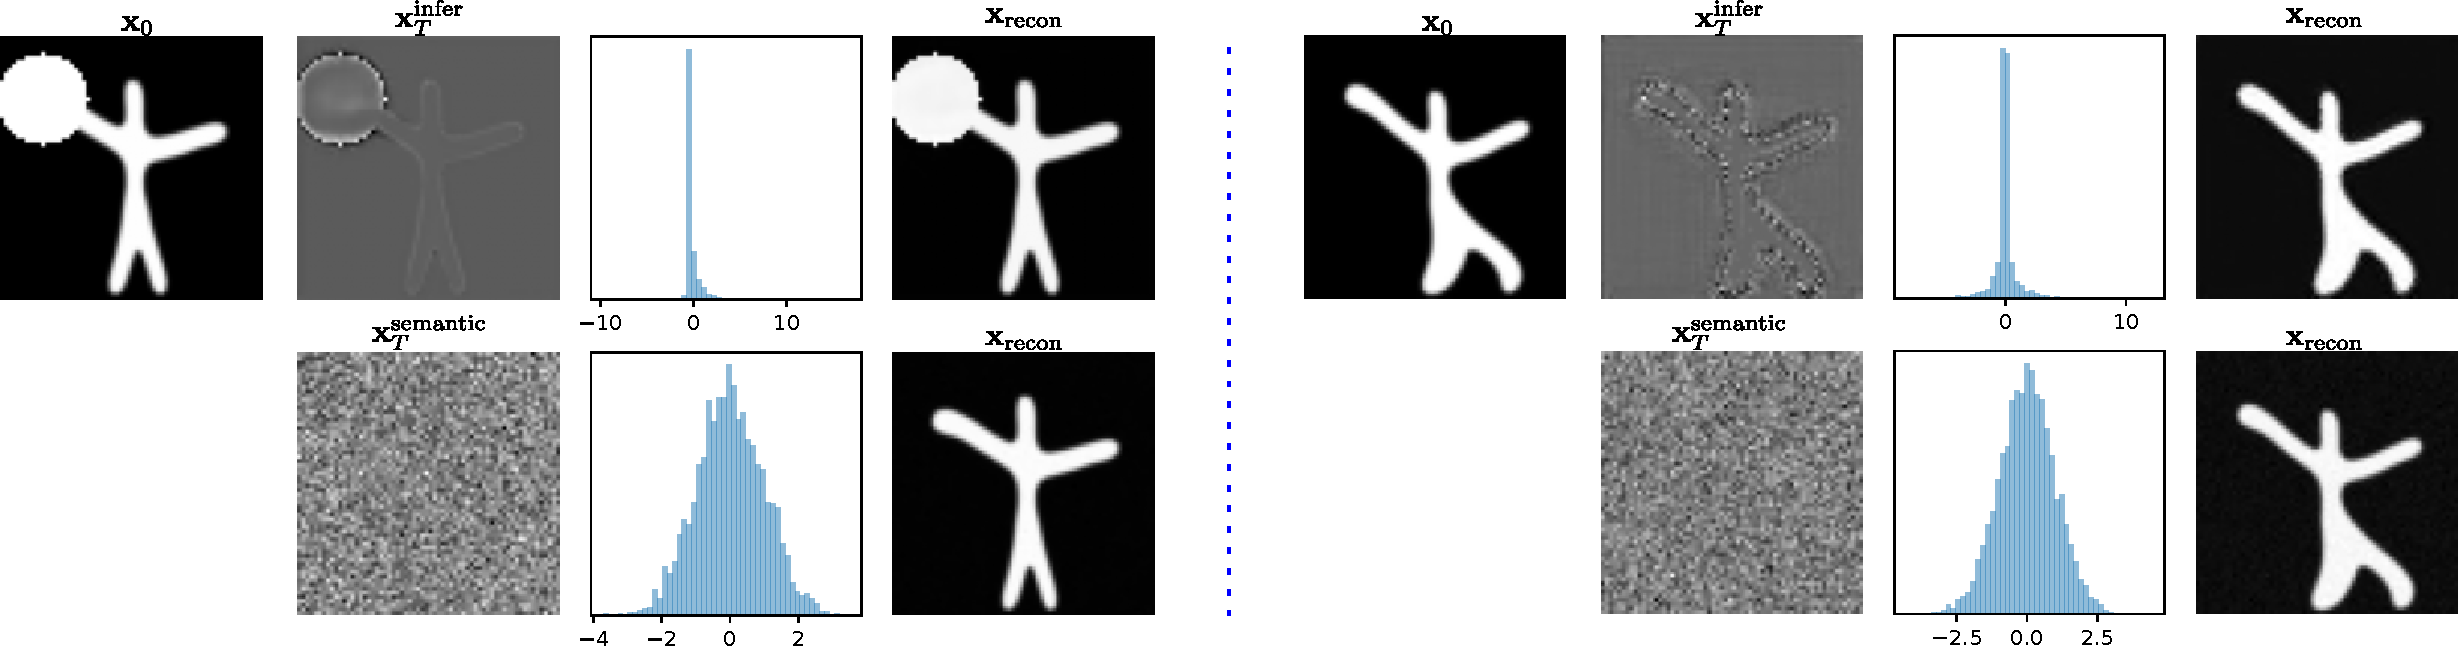
\includegraphics[width=0.75\linewidth]{figures/compare-infer-hist.pdf}
    \caption[Histogram of intensity of random noise and stochastic subcode]{The histogram of intensity of $\rvx_T^{\text{infer}}$ compared to normal noisy $\rvx_T^{\text{semantic}}$, and their corresponding reconstruction. Left: example from anomaly image. Right: example from healthy image.}
    \label{fig:compare-infer-hist}
\end{figure}

\subsection{Effect of noise level on reconstruction errors}
In this section, we investigate the effect of added noise to reconstruction error. \cref{tab:compare-noise-levels} presents the reconstruction errors for different noise levels applied to the input image. We test several noise level from 50 to 1000, with 1000 means that the denoising process starts from pure random Gaussian noise. We observe that lower noise levels (50 and 100) yield better reconstruction quality for healthy anatomy, as indicated by lower $l1$-error and higher SSIM and PSNR values. However, these noise levels result in lower anomaly reconstruction errors, which is undesirable for UAD tasks. Conversely, higher noise levels (750, 800, and 1000) lead to increased anomaly reconstruction errors but also higher reconstruction errors for healthy anatomy. The optimal balance is achieved at a noise level of 250, which provides a good trade-off between accurately reconstructing healthy anatomy and effectively removing anomalies. This result is inline with the \emph{noise paradox} discussed in \cite{autoDDPM}.  

\cref{tab:compare-noise-level-anomalies} provides a detailed breakdown of reconstruction errors for each anomaly type across different noise levels. We observe that the \texttt{growing\_circle} anomaly (large and more noticeable anomalies) type shows the most significant increase in anomaly reconstruction error as the noise level increases, while the \texttt{darker\_line} and \texttt{darker\_circle} (more subtle) anomaly types show more moderate increases. This suggests that the effectiveness of anomaly removal may vary depending on the nature of the anomaly and its contrast with the surrounding healthy tissue. Anomaly with higher intensity needs more noise to be effectively removed, while subtle anomalies require more moderate nosie levels and need more dedicated handling to preserve healthy anatomy.

\begin{table}[h]
    \centering
    \resizebox{1.\textwidth}{!}{
    \begin{tabular}{lrrrrrrrr}
    \toprule
     & \multicolumn{5}{c}{Healthy} & \multicolumn{3}{c}{Anomalies} \\
     \cmidrule(lr){2-6} \cmidrule(lr){7-9}
     & $l$1-error(1e-3)$\downarrow$ & SSIM(\%) $\uparrow$ & MSSIM(\%) $\uparrow$ & PSNR $\uparrow$& LPIPS(1e-3) $\downarrow$ & $l$1-Ano(1e-3) $\uparrow$& $l$1-Healthy(1e-3)$\downarrow$ & $l$1-ratio $\uparrow$\\
    Noise level &  &  &  &  &  &  &  &  \\
    \midrule
    50 & \textbf{10.678} & 84.771 & 98.864 & \textbf{36.908} & 38.093 & 323.192 & \textbf{11.737} & 27.537 \\
    100 & 11.132 & 85.222 & \textbf{98.902} & 35.697 & 35.431 & 508.632 & 12.076 & 42.119 \\
    250 & 12.615 & 85.694 & 98.852 & 32.655 & 32.041 & 653.881 & 13.111 & \textbf{49.873} \\
    400 & 13.704 & \textbf{85.806} & 98.751 & 31.084 & 30.399 & 666.405 & 14.070 & 47.365 \\
    500 & 14.273 & 85.586 & 98.677 & 30.508 & 30.457 & 669.581 & 14.628 & 45.775 \\
    600 & 14.642 & 85.486 & 98.635 & 30.162 & \textbf{30.288} & 671.424 & 14.999 & 44.763 \\
    750 & 15.250 & 84.954 & 98.547 & 29.850 & 31.434 & 672.778 & 15.598 & 43.133 \\
    800 & 15.420 & 84.885 & 98.513 & 29.793 & 31.366 & 673.050 & 15.759 & 42.708 \\
    1000 & 17.953 & 83.505 & 97.989 & 29.539 & 34.377 & \textbf{674.115} & 18.192 & 37.056 \\
    \bottomrule
    \end{tabular}
    }
    \caption[Effects of noise level on reconstruction errors]{The effects of applying different noise levels on reconstruction errors. Arrows $\uparrow$ and $\downarrow$ indicate that higher and lower values are favorable, respectively. The best results are highlighted in \textbf{bold}. Results for the anomalous datasets represent the average over all three types of anomalies.}
    \label{tab:compare-noise-levels}
\end{table}

\begin{table}[h]
    \centering
    \resizebox{1.\textwidth}{!}{
    \begin{tabular}{lrrrrrrrrr}
    \toprule
     & \multicolumn{3}{c}{growing circle} & \multicolumn{3}{c}{darker line} & \multicolumn{3}{c}{darker circle} \\
     \cmidrule(lr){2-4} \cmidrule(lr){5-7} \cmidrule(lr){8-10}
     & $l$1-Ano(1e-3) $\uparrow$& $l$1-Healthy(1e-3)$\downarrow$ & $l$1-ratio $\uparrow$ & $l$1-Ano(1e-3) $\uparrow$& $l$1-Healthy(1e-3)$\downarrow$ & $l$1-ratio $\uparrow$ & $l$1-Ano(1e-3) $\uparrow$& $l$1-Healthy(1e-3)$\downarrow$ & $l$1-ratio $\uparrow$ \\
    Noise level &  &  &  &  &  &  &  &  &  \\
     \midrule
    50 & 313.516 & 18.810 & 16.668 & 352.260 & 12.660 & 27.824 & 349.308 & \textbf{11.849} & 29.480 \\
    100 & 553.121 & 19.249 & 28.735 & 384.994 & \textbf{12.228} & \textbf{31.486} & 372.165 & 11.993 & \textbf{31.031} \\
    250 & 743.802 & 16.359 & 45.467 & 399.816 & 13.063 & 30.608 & 384.890 & 13.706 & 28.081 \\
    400 & 759.369 & \textbf{15.821} & \textbf{47.998} & 403.404 & 13.983 & 28.851 & 388.863 & 15.188 & 25.604 \\
    500 & 763.256 & 15.957 & 47.831 & 404.529 & 14.598 & 27.711 & 389.978 & 16.020 & 24.343 \\
    600 & 765.465 & 16.096 & 47.557 & 405.295 & 14.983 & 27.051 & 390.802 & 16.633 & 23.495 \\
    750 & 767.102 & 16.423 & 46.709 & 405.784 & 15.375 & 26.393 & 391.408 & 17.630 & 22.201 \\
    800 & 767.445 & 16.445 & 46.668 & \textbf{405.840} & 15.404 & 26.346 & 391.492 & 17.997 & 21.754 \\
    1000 & \textbf{768.724} & 17.109 & 44.931 & 405.403 & 16.318 & 24.845 & \textbf{393.398} & 22.926 & 17.159 \\
    \bottomrule
    \end{tabular}
    }
    \caption[Reconstruction errors with different noise levels on anomalous subjects]{Details of reconstruction errors with different noise levels on anomaly datasets. Best results are highlighted in \textbf{bold}}
    \label{tab:compare-noise-level-anomalies}
\end{table}

\section{Unsupervised Anomaly Detection}
In this section, we present the result of anomaly detection using psuedo-healthy image from trained SDM model. All reconstructed images are obtained by denoising from $\rvx_T^{\text{infer}}$ (adding random Gaussian noise to original image). All experiences are done with added noise level of 250, and DDIM sampling is used with 100 denoising steps. 

\begin{figure}
    \centering
    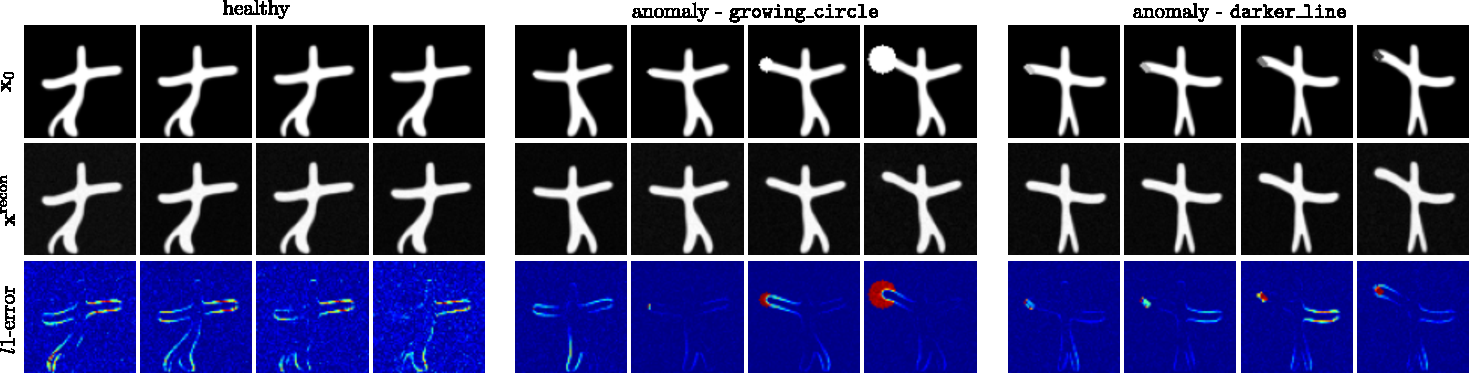
\includegraphics[width=1\linewidth]{figures/ex-recon-error.pdf}
    \caption[Example of $l1$-error for healthy and anomalous subjects]{Example of residual error $l1$-error for healthy and anomaly subjects. From top to bottom: original image, reconstructed image, and residual error. Left: healthy subject. Middle: anomaly subject with \texttt{growing\_circle}. Right: anomaly subject with \texttt{darker\_line}. Note that the color code is not on the same scale for all images.}
    \label{fig:example-recon-error}
\end{figure}

\cref{fig:example-recon-error} shows examples of residual error ($l1$-error) for healthy and anomaly subjects. Visually, the anomaly part can be detected by the high residual error, relatively compared to other parts of the image. However, choosing a proper threshold is proven to be non-trivial, as we can observe high residual error in some healthy parts due to reconstruction quality. This leads to high false positive rate when using simple threshold methods. We can follow some post processing steps from existing literature, such as removing small connected components, but this approach requires prior knowledge about the size of anomalies \cite{behrendt2025cDDPM}. In this work, we target subtle anomaly type for Parkinson disease, and we do not want to make any assumption about the anomaly size. On the other hand, we see that at early stage of disease progression, when the anomaly is very small, residual error is hard to distinguish from other healthy parts. This leads to false negative challenge, which can be more detrimental in clinical screening. \cref{fig:example-seg} shows the results of using naive quantile threshold methods: it generates extremely high false positive rate, for both healthy and anomalous subjects. 

\subsection{Anomaly segmentation with Feature Attention Module}

To address the shortcomings of the pixel residual map, our \ac{FAM} module is designed to attend to the information from the feature distance between the original images and their pseudo-healthy reconstructions. Unlike pixel distance, feature distance focuses more on perceptual differences between two images, highlighting errors only when there is a distortion in the overall image structure. \ac{FAM} learns to ignore minor pixel residuals (reconstruction errors) from our trained FE network $\Phi$ (\cref{sec:feature-extractor-network}). 

\begin{figure}[h]
    \centering
    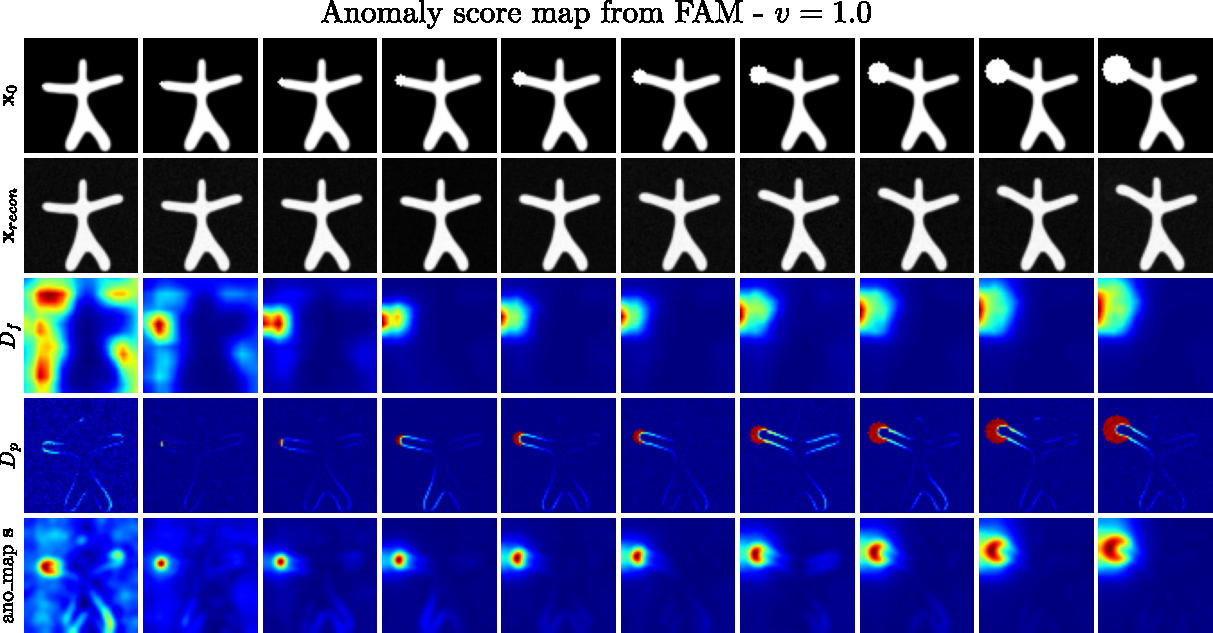
\includegraphics[width=0.75\linewidth]{figures/ano-score-map-gcircle.pdf}
    \caption[Anomaly score map from FAM]{Anomaly score map as combination of feature distance and pixel distance. From top to bottom: original image, reconstructed image, pixel distance, feature distance, and anomaly score map as combination of both. The hyperparameter is $v=1$.}
    \label{fig:ano-score-map-gcircle}
\end{figure}

\cref{fig:ano-score-map-gcircle} shows the anomaly score maps from \ac{FAM} as a combination of feature distance $D_f$ and pixel distance $D_p$. The feature distance correctly captures the overall structural changes in the image. By combining $D_f$ and $D_p$, \ac{FAM} reduces reconstruction errors and shifts the focus to regions with high residual and perceptual errors. However, when anomalies are small and subtle (at an earlier stage), we still encounter false negatives—for example, the residual error in the correct region may be relatively small compared to other healthy regions. Note that the color code in \cref{fig:ano-score-map-gcircle} are not on the same scale. At time $l=0$, the red region indicates the highest value in the feature distance map, but the actual feature error there is very small (close to 0), as shown in \cref{fig:hist-fd-id-gcircle}.

\begin{figure}[h]
    \centering
    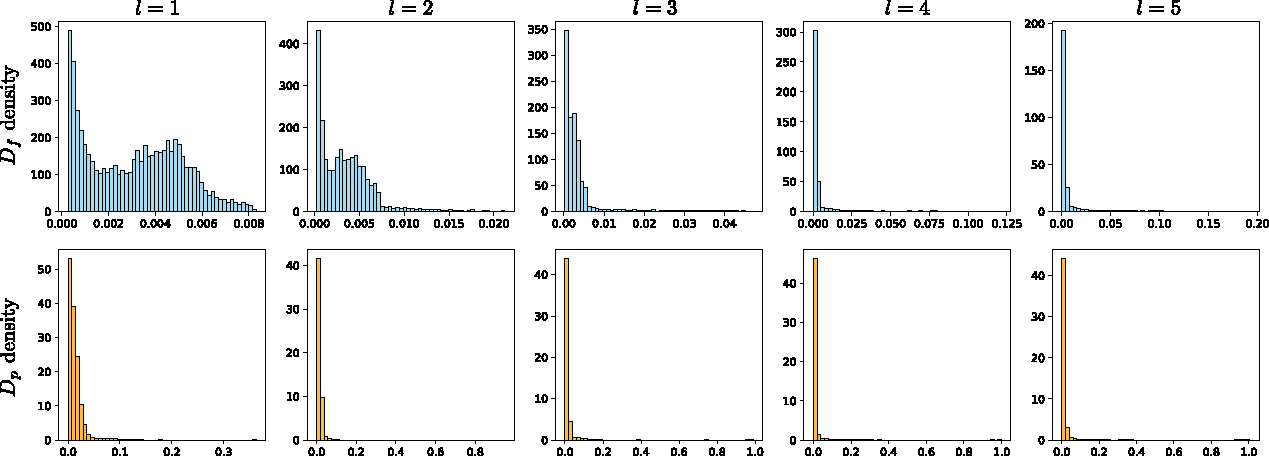
\includegraphics[width=0.75\linewidth]{figures/hist-fd-id-gcircle.pdf}
    \caption[Example of normalized histogram of $D_f$ and $D_p$]{Example of normalized histogram of feature distance $D_f$ (top row) and pixel distance $D_p$ (bottom row) for different time points $l$. }
    \label{fig:hist-fd-id-gcircle}
\end{figure}

\cref{fig:hist-ano-map} shows the effect of using \ac{FAM} on the pixel distance map. For anomalous subjects, the normalized histogram of residual errors is not a reliable indicator for separating anomalous pixels from healthy ones. By using the feature distance, \ac{FAM} spreads out the histogram of residual errors, making it easier to apply automatic thresholding or quantile-based methods to localize anomaly regions.

\begin{figure}[h]
    \centering
    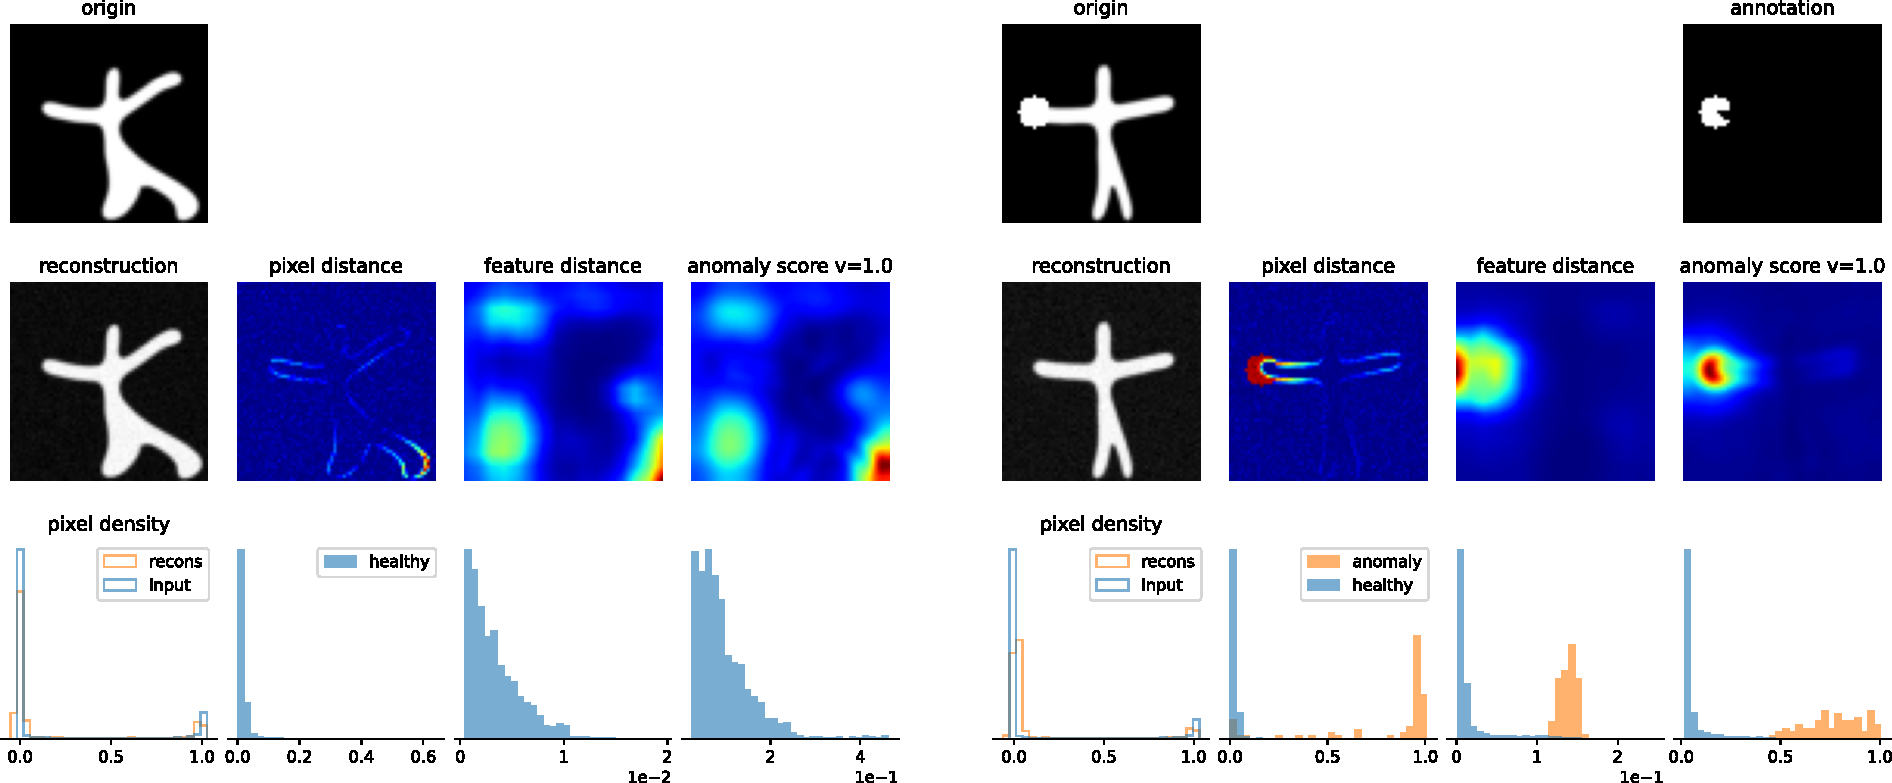
\includegraphics[width=1\linewidth]{figures/hist-ano-map.pdf}
    \caption[Effect of FAM on anomaly score map]{The effect of combination of feature distance and pixel distance. Left: example of healthy image. Right: example of anomaly image. The hyperparameter is $v=1$}
    \label{fig:hist-ano-map}
\end{figure}

\begin{figure}[htbp]
    \centering
    \begin{subfigure}{0.75\textwidth}
        \centering
        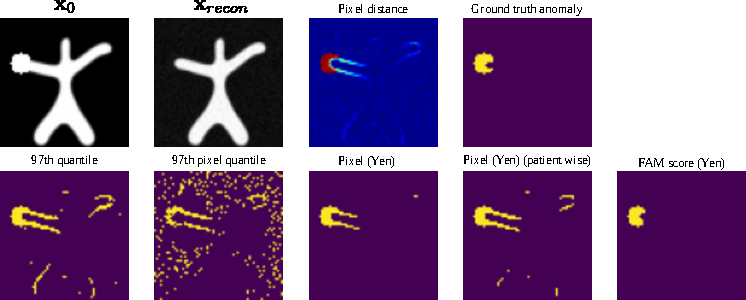
\includegraphics[width=1.0\linewidth]{figures/compare-pix-seg-gcircle.pdf}
        \caption{Anomaly subject.}
        \label{fig:example-seg-gcircle}
    \end{subfigure}
    \hfill
    \begin{subfigure}{0.75\textwidth}
        \centering
        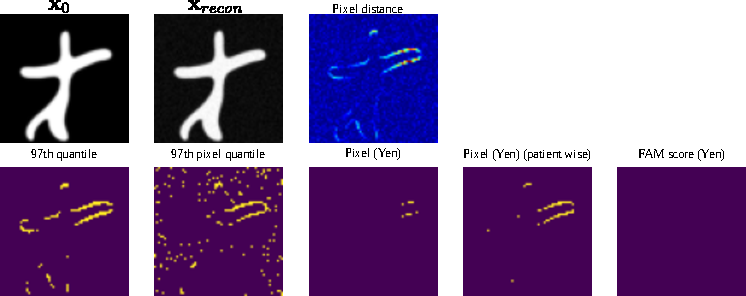
\includegraphics[width=1.0\linewidth]{figures/compare-pix-seg-healthy.pdf}
        \caption{Healthy subject.}
        \label{fig:example-seg-healthy}
    \end{subfigure}
    \hfill
    \begin{subfigure}{0.75\textwidth}
    \centering
    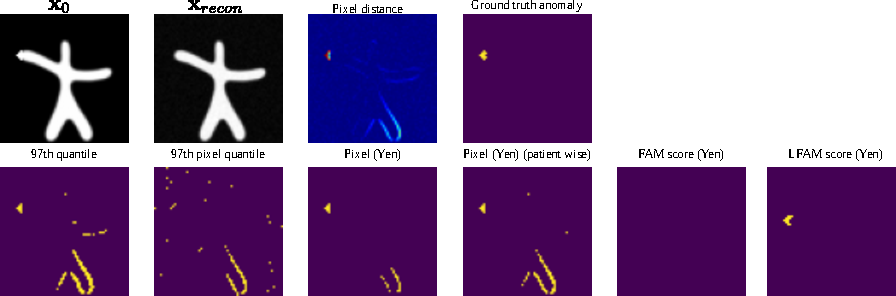
\includegraphics[width=1.0\linewidth]{figures/compare-pix-seg-healthy-false-neg.pdf}
    \caption{Anomaly subject (subtle).}
    \label{fig:example-seg-gcircle-false-neg}
\end{subfigure}
    \caption[Example of anomaly segmentation with different methods]{Example of anomaly segmentation using different methods. \cref{fig:example-seg-gcircle} and \cref{fig:example-seg-gcircle-false-neg} show examples of anomaly subjects, while \cref{fig:example-seg-healthy} shows an example of a healthy subject. The first row: original image, reconstructed image, residual error, and ground truth anomaly segmentation (if any). The second row: segmentation using image-wise 97\% quantile, pixel-wise 97\% quantile, dataset-wise Yen thresholding, patient-wise Yen thresholding, and anomaly score map with \ac{FAM}.}
    \label{fig:example-seg}
\end{figure}

\cref{tab:dice-methods} reports the quantitative results of mDICE scores for different thresholding methods. For the healthy dataset, we also report the false positive percentage (FP\%), i.e., the proportion of the image area incorrectly marked as anomalous. Pixel-quantile methods compute the quantile for each pixel individually, while quantile methods compute it over the whole image (dataset-wise). Yen method applies Yen automatic threshold technique to the pixel distance map $D_p$. \ac{FAM} calculates the anomaly score map by combining feature distance and pixel distance. Quantile methods are applied to the entire test dataset. For the Yen and \ac{FAM} methods, results are reported for both dataset-wise and patient-wise thresholds. The dataset-wise method computes a single threshold value for the whole test dataset (including both healthy and anomalous images). The patient-wise method computes one threshold per patient, considering all observations for that patient (10 observations per patient).

We observe that the classic quantile methods perform poorly in terms of both false positive rates and mDICE scores. The Yen method achieves strong anomaly segmentation performance, attaining some of the highest mDICE scores, except for the \texttt{growing\_circle} anomaly type, where the \ac{FAM} method achieves higher segmentation quality. Moreover, \ac{FAM} yields the best results in terms of minimizing the false positive rate in healthy regions. The result indicates that Yen method has the best overall mDICE score of $69\%$ only if we use the whole dataset to calculate threshold, which increase almost 10\% compared to patient-wise result of $58\%$. We see similar results for \ac{FAM} method, where all mDICE score is higher when the threshold is calculated dataset-wise. This is expected, as having more data provides better information to separate healthy and anomalous pixels. On the other hand, FP is best with patient-wise method. 

\cref{fig:example-seg} displays examples of anomaly localization results for different methods. It is clear that the quantile methods perform poorly, as they fail to disentangle anomaly errors from model reconstruction errors. For healthy subjects, \ac{FAM} outperforms the Yen method in minimizing false positive segmentations.

\begin{table}[htbp]
    \centering
    \resizebox{1.\textwidth}{!}{
    \begin{tabular}{lrrrrrr}
    \toprule
    & & \multicolumn{1}{c}{Healthy} & \multicolumn{4}{c}{Anomaly} \\
    \cmidrule(lr){3-3} \cmidrule(lr){4-7} 
     & &  & growing circle & darker circle & darker line & Total \\
    \multicolumn{2}{c}{Methods} & FP (\%) $\downarrow$ & mDICE\% $\uparrow$ & mDICE\% $\uparrow$ & mDICE\% $\uparrow$ & mDICE\% $\uparrow$ \\
    \midrule
    \multirow{5}{*}{Pixel quantile} & q90.0 & 9.081 & 16.526 & 6.477 & 11.751 & 11.585 \\
                                    & q92.5 & 6.702 & 19.513 & 7.572 & 14.354 & 13.813 \\
                                    & q95.0 & 4.310 & 23.718 & 8.039 & 16.960 & 16.239 \\
                                    & q97.5 & 2.041 & 27.565 & 7.193 & 16.743 & 17.167 \\
                                    & q99.0 & 0.734 & 24.889 & 4.551 & 10.016 & 13.152 \\
    \midrule
    \multirow{5}{*}{Quantile}      & q90.0 & 9.152 & 17.125 & 6.663 & 11.592 & 11.793 \\
                                    & q92.5 & 6.768 & 20.953 & 8.592 & 14.577 & 14.707 \\
                                    & q95.0 & 4.435 & 28.061 & 12.165 & 19.784 & 20.004 \\
                                    & q97.5 & 2.122 & 42.638 & 22.375 & 33.193 & 32.736 \\
                                    & q99.0 & 0.684 & 60.276 & 44.588 & 57.832 & 54.232 \\
    \midrule
    \multirow{2}{*}{Pixel score (Yen)} & dataset wise       & 0.192 & \textbf{76.867} & 59.600 & 70.683 & \textbf{69.050} \\
                                    & patient wise & 1.645 & 47.369 & 58.500 & \textbf{70.872} & 58.914 \\
    \midrule
    \multirow{2}{*}{\shortstack{Anomaly score map \\ FAM}} & dataset wise      & 0.204 & 60.531 & \textbf{65.254} & 62.455 & 62.747 \\
                                        & patient wise & \textbf{0.059} & 57.782 & 49.798 & 44.877 & 50.819 \\
    \bottomrule
    \end{tabular}
    }
    \caption[FP\% and DICE\% for different method]{DICE scores for the anomaly segmentation task, reported for different methods. For anomaly subjects, \texttt{Total} is the average of mDICE scores for all anomaly types. Best results are highlighted in \textbf{bold}.}
    \label{tab:dice-methods}
\end{table}

Notably, one drawback of applying thresholding techniques dataset-wise is that the results strongly depend on the composition of the dataset. Our test dataset comprises 150 healthy subjects and 60 anomalous subjects (20 for each type of anomaly), meaning that approximately 70\% of the samples are healthy. Because healthy images have smaller residual errors, having more healthy references helps to better highlight anomalous regions. \cref{fig:fp-mdice-compare} and \cref{tab:fp-mdice-nb-healthy} illustrate the fluctuations in FP and mDICE scores for different dataset compositions. In particular, we vary the number of healthy subjects while fixing the number of anomalous ones. 

\begin{figure}[htbp]
    \centering
    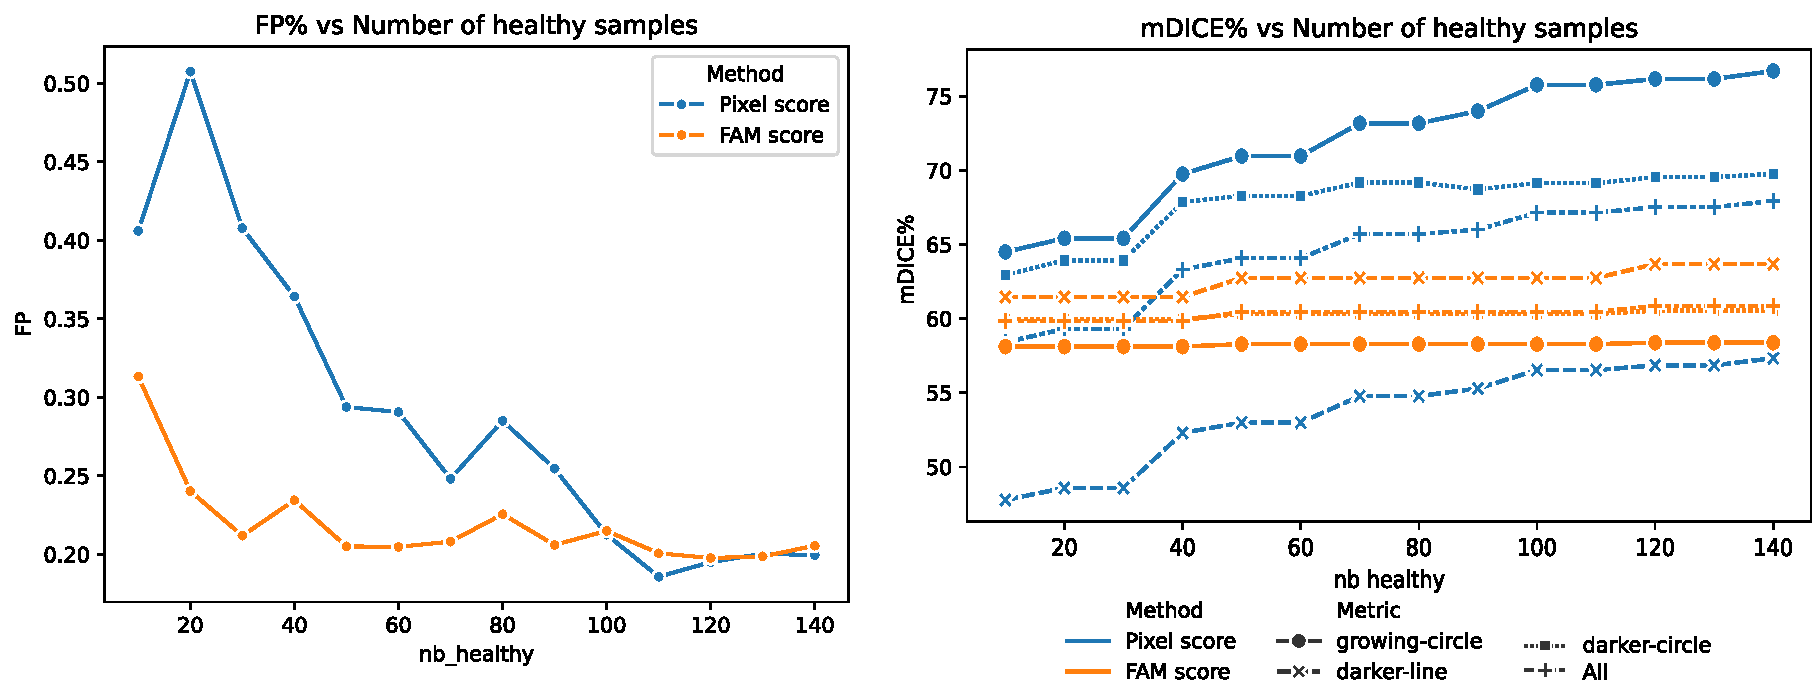
\includegraphics[width=0.9\linewidth]{figures/metric-vs-nb-healthy.pdf}
    \caption[FP(\%) and mDICE(\%) for different unbalanced compositions of dataset]{FP(\%) and mDICE(\%) scores for different unbalanced compositions of the test dataset. Left: FP \% for healthy patients. Right: mDICE \% score for the anomaly segmentation task. The x-axis denotes the number of healthy patients in the dataset, the number of anomalous patients is fixed at 60.}
    \label{fig:fp-mdice-compare}
\end{figure}

As expected, mDICE scores increase as the number of healthy references grows. One interesting observation is that, while the Yen method achieves a higher mDICE score than FAM, FAM demonstrates more stable performance, maintaining consistent scores across different numbers of healthy observations. For false positive rates, FAM also exhibits smaller fluctuations than the Yen method, although we do not see the same consistency as for mDICE.

\begin{table}[htbp]
    \centering
    \resizebox{\textwidth}{!}{%
    \begin{tabular}{lrrrrrrrrrr}
    \toprule
     & \multicolumn{5}{c}{Pixel distance (Yen threshold)} & \multicolumn{5}{c}{Feature Attention Module} \\
     % & \multicolumn{1}{c}{healthy} & \multicolumn{4}{c}{anomaly (mDICE\%)} \\
    \cmidrule(lr){2-6} \cmidrule(lr){7-11}
    & healthy & growing-circle & darker-line & darker-circle & All & healthy & growing-circle & darker-line & darker-circle & All \\
    nb healthy & FP(\%) \textdownarrow & mDICE\% \textuparrow & mDICE\% \textuparrow & mDICE\% \textuparrow & mDICE\% \textuparrow & mDICE\% \textuparrow & mDICE\% \textuparrow & mDICE\% \textuparrow & mDICE\% \textuparrow & mDICE\% \textuparrow \\
    \midrule
    10 & 0.401 & 65.986 & 51.072 & 64.600 & 60.553 & 0.240 & 60.068 & 61.929 & 61.460 & 61.152 \\
    20 & 0.379 & 66.804 & 51.798 & 65.485 & 61.362 & 0.213 & 60.068 & 61.929 & 61.460 & 61.152 \\
    30 & 0.415 & 68.433 & 53.291 & 67.230 & 62.985 & 0.247 & 60.298 & 63.275 & 61.945 & 61.839 \\
    40 & 0.331 & 68.433 & 53.291 & 67.230 & 62.985 & 0.178 & 60.298 & 63.275 & 61.945 & 61.839 \\
    50 & 0.268 & 70.670 & 55.110 & 68.992 & 64.924 & 0.186 & 60.445 & 64.423 & 62.263 & 62.377 \\
    60 & 0.348 & 71.752 & 55.728 & 69.356 & 65.612 & 0.209 & 60.445 & 64.423 & 62.263 & 62.377 \\
    70 & 0.253 & 71.752 & 55.728 & 69.356 & 65.612 & 0.171 & 60.445 & 64.423 & 62.263 & 62.377 \\
    80 & 0.241 & 74.453 & 57.774 & 69.748 & 67.325 & 0.220 & 60.445 & 64.423 & 62.263 & 62.377 \\
    90 & 0.244 & 75.114 & 58.066 & 69.651 & 67.611 & 0.211 & 60.445 & 64.423 & 62.263 & 62.377 \\
    100 & 0.218 & 75.247 & 58.504 & 69.803 & 67.851 & 0.204 & 60.445 & 64.423 & 62.263 & 62.377 \\
    110 & 0.204 & 76.033 & 58.883 & 70.128 & 68.348 & 0.194 & 60.531 & 65.254 & 62.455 & 62.747 \\
    120 & 0.210 & 76.386 & 59.171 & 70.480 & 68.679 & 0.203 & 60.531 & 65.254 & 62.455 & 62.747 \\
    130 & 0.200 & 76.386 & 59.171 & 70.480 & 68.679 & 0.211 & 60.531 & 65.254 & 62.455 & 62.747 \\
    140 & 0.197 & 76.867 & 59.600 & 70.683 & 69.050 & 0.201 & 60.531 & 65.254 & 62.455 & 62.747 \\
    \bottomrule
    \end{tabular}%
    }
    \caption[FP\% and DICE\% for different compositions of test dataset]{FP(\%) and mDICE(\%) results for different numbers of healthy patients in the test dataset. The number of anomaly patients is fixed at 60. The left part of the table shows results using Yen threshold on pixel distance, while the right part shows results using the Feature Attention Module (FAM).}
    \label{tab:fp-mdice-nb-healthy}
\end{table}

In a real case scenario, we do not know the real composition of our test dataset, and ideally we want to improve our method so that it only depends on information per patient, making it more robust for unbalanced dataset. Also, FAM mainly solves the problem of false positive, but for real anomaly detection its performance is still inferior to normal automatic Yen threshold method. \cref{fig:example-seg-gcircle-false-neg} shows 1 example where FAM fails to detect subtle anomaly, while Yen method can detect the anomaly but also include other healthy regions. In the next section, we present our result for anomaly segmentation with our proposed Longitudinal Attention Fusion Module. 

\subsection{Anomaly segmentation with Longitudinal Attention Fusion Module}
By fussing the information from multiple time points, \ac{LAFM} aims to improve the accuracy of anomaly detection, both reducing false positives (anomalies that do not persist over time) and false negatives (use anomalies that are detected from future time points to help detect subtle anomalies at earlier time points).

\begin{table}[]
    \centering
    % \resizebox{1.\textwidth}{!}{%
    \begin{adjustbox}{max width=\textwidth}
    \begin{tabular}{lrrrrr}
    \toprule
     & \multicolumn{1}{c}{Healthy} & \multicolumn{4}{c}{Anomalies} \\
     \cmidrule(lr){2-2} \cmidrule(lr){3-6} 
    & healthy & growing circle & darker circle & darker line & All \\
    methods & FP(\%) \textdownarrow & mDICE\% \textuparrow & mDICE\% \textuparrow & mDICE\% \textuparrow & mDICE\% \textuparrow \\
    \midrule
    Pixel score (dataset wise) & 0.192 & 76.867 & 59.600 & 70.683 & 69.050 \\
    Pixel score (patient wise) & 1.645 & 47.369 & 58.500 & 70.872 & 58.914 \\
    \midrule
    FAM (dataset wise) & 0.204 & 60.531 & 65.254 & 62.455 & 62.747 \\
    FAM (patient wise) & \textbf{0.059} & 57.782 & 49.798 & 44.877 & 50.819 \\
    \midrule
    LAFM ($\sigma=0.0$) & 0.169 & 84.790 & 81.665 & 86.924 & 84.460 \\
    LAFM ($\sigma=0.5$) & 0.198 & 82.441 & \textbf{82.784} & \textbf{87.950} & 84.391 \\
    LAFM ($\sigma=1.0$) & 0.191 & 82.893 & 81.926 & 87.891 & 84.237 \\
    LAFM ($\sigma=1.5$) & 0.178 & 83.604 & 82.682 & 87.909 & 84.731 \\
    LAFM ($\sigma=2.0$) & 0.207 & 85.540 & 81.997 & 87.634 & 85.057 \\
    LAFM ($\sigma=2.5$) & 0.183 & \textbf{86.069} & 81.981 & 87.352 & \textbf{85.134} \\
    LAFM ($\sigma=3.0$) & 0.184 & 85.995 & 81.779 & 87.304 & 85.026 \\
    LAFM ($\sigma=3.5$) & 0.198 & 85.890 & 81.648 & 86.929 & 84.823 \\
    LAFM ($\sigma=4.0$) & 0.194 & 85.762 & 81.826 & 86.893 & 84.827 \\
    LAFM ($\sigma=4.5$) & 0.183 & 85.783 & 81.683 & 86.779 & 84.748 \\
    \bottomrule
    \end{tabular}
    \end{adjustbox}
    %}
    \caption[FP\% and DICE\% for different method - with LAFM]{mDICE and FP scores for different anomaly segmentation methods. The best results are highlighted in \textbf{bold}.}
    \label{tab:dice-lafm}
\end{table}

\cref{tab:dice-lafm} reports anomaly segmentation metrics using LAFM with different variants of Gaussian smoothing $\sigma$. Here, $\sigma=0$ indicates that time points are weighted equally. As discussed in \cref{sec:method-lafm}, $\sigma$ controls the contribution of anomaly score maps from surrounding time points, depending on their distance from the current target image. The mDICE metric increases to around $86\%$, compared to $62\%$ and $69\%$ for FAM and Yen, respectively. LAFM only underperforms FAM in terms of the FP metric, but its result is still comparable to the Yen method, with an acceptable rate of around $0.19\%$. This highlights the trade off between FP and FN: method that achieves the best FP rate processes the residual error more conservatively at the cost of potentially missing some anomalies. On the other hand, method with higher segmentation accuracy will increase the likelihood of anomalies, which leads to more healthy regions being flagged as anomaly. 

\cref{fig:lafm-seg-gcircle} shows 1 example of anomaly segmentation from LAFM. We see that by using information from other time points, we can refine the anomaly map by adding anomaly regions that persist across time and reducing potential anomalies that do not. This effect is more apparent at earlier stages, for example, in the first two time points.

\begin{figure}[htbp]   
    \centering
    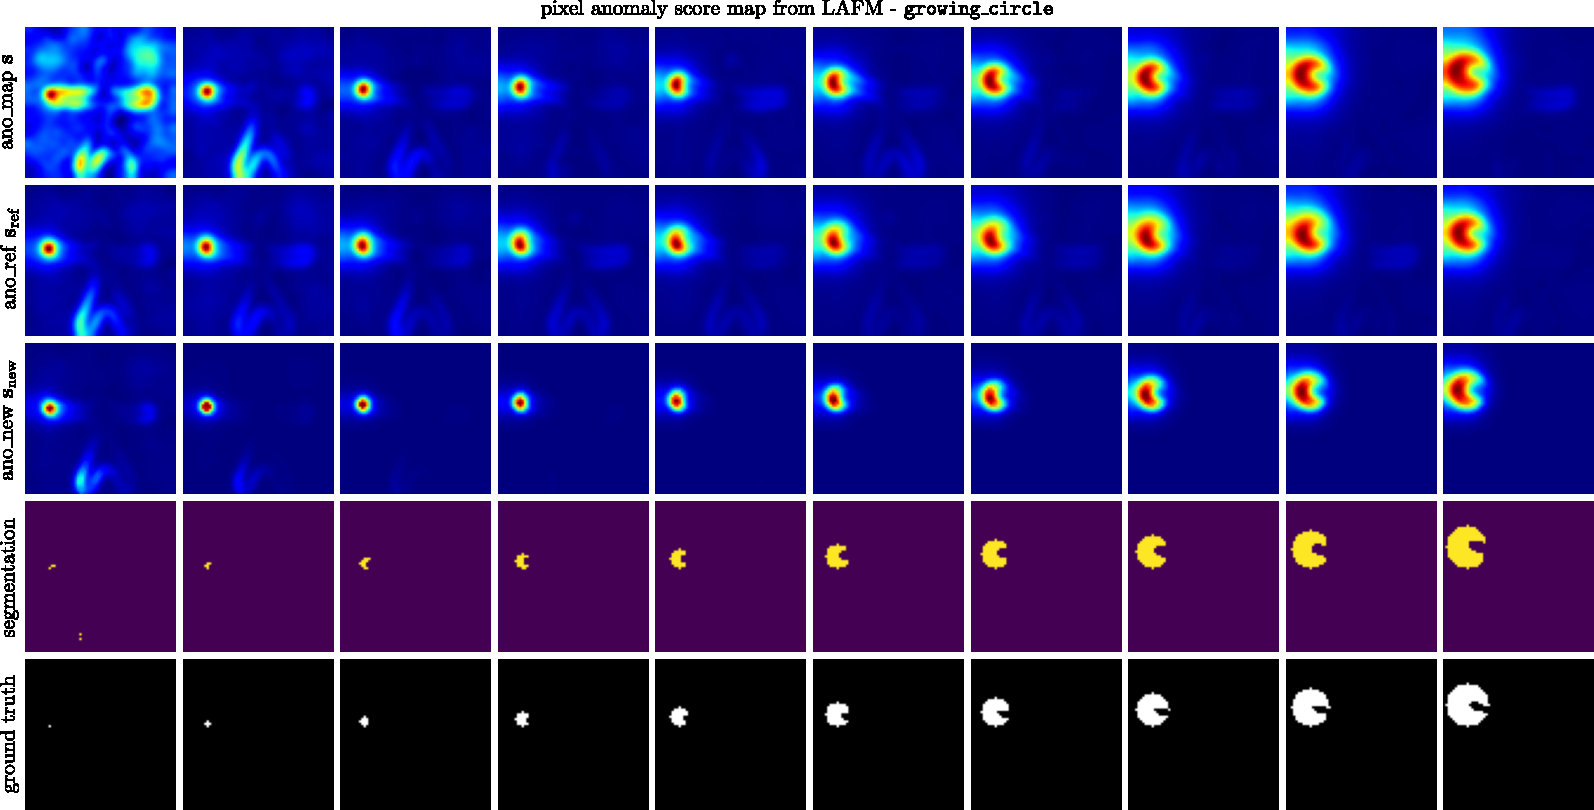
\includegraphics[width=0.75\linewidth]{figures/lafm-seg-gcircle.pdf}
    \caption[Anomaly segmentations from LAFM]{Anomaly segmentation from LAFM. From top to bottom: anomaly map (targeted image), anomaly map references from other time points, updated anomaly map based, anomaly segmentation and ground truth annotation.}
    \label{fig:lafm-seg-gcircle}
\end{figure}

One disadvantage of LAFM is that its performance depends on the number of observations for each patient. The more observations we have, the more additional information we can use to improve the current prediction. \cref{fig:lafm-varying-nbseen} shows the performance of Yen, FAM and LAFM with different numbers of observations (per patient). For each experience, we randomly choose $n$ samples for each patient's longitudinal samples ($\mathrm{max}(n) = 10$). We note that for each $n$, the interval between time points $\Delta_l$ are random. Since the referenced anomaly score maps are weighted by a Gaussian kernel that depends on $\Delta_l$, this randomness can affect the overall performance. To account for this, we run the experience 10 times and reports the average results. 

\begin{figure}[htbp]   
    \centering
    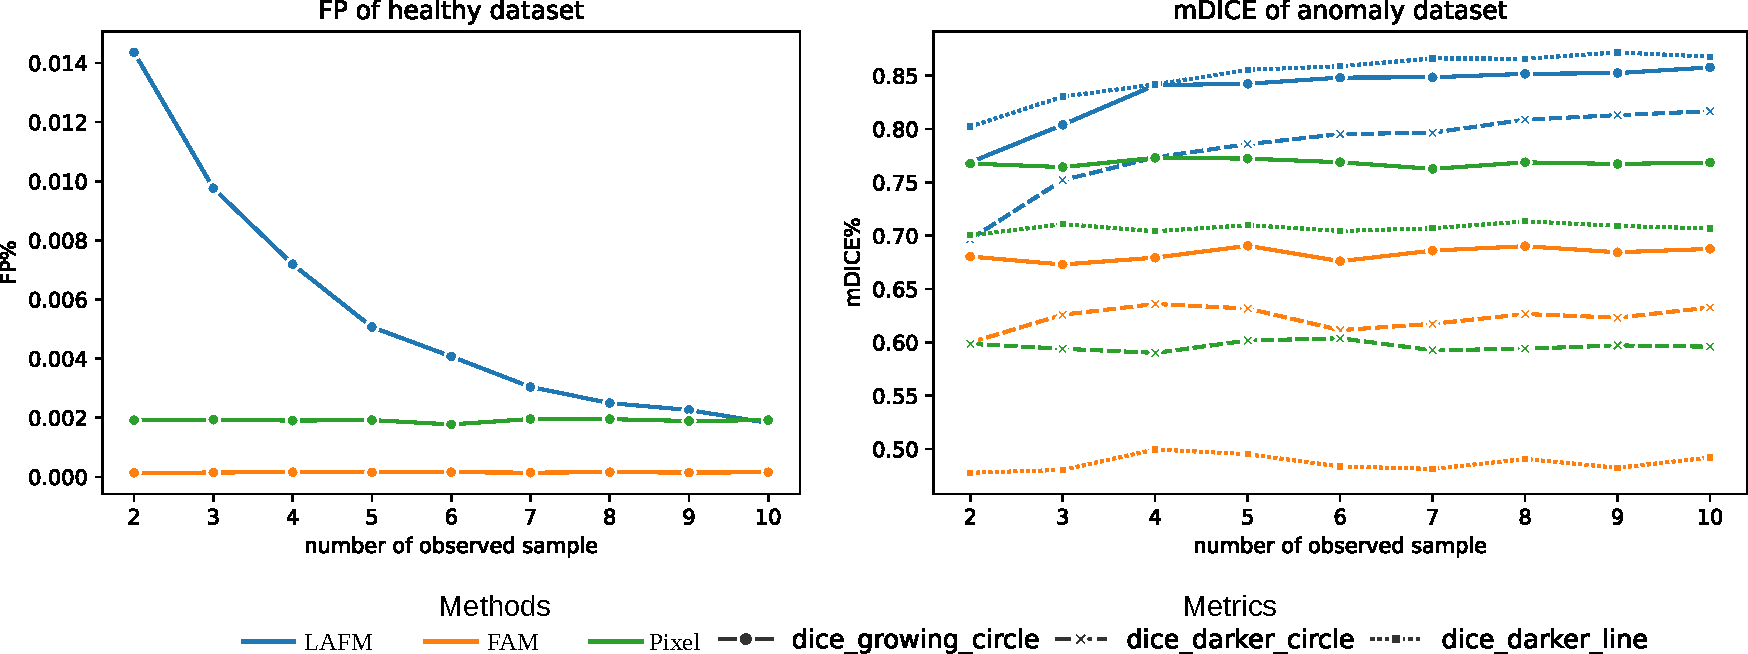
\includegraphics[width=1.0\linewidth]{figures/lafm-varying-nbseen.pdf}
    \caption[FP\% and mDICE\% scores for different numbers of observations]{Comparison of FP\% and mDICE\% scores for different numbers of observed time points. Results for LAFM is calculated with $\sigma=0.5$.}
    \label{fig:lafm-varying-nbseen}
\end{figure}

We see that Yen and FAM have small fluctuations with different number of observations, while LAFM's performance increases as we have more observations. mDICE increases significantly from 2 to 4 observations, and from 4 observations onward, LAFM starts outperforming Yen. On the other hand, FP only reaches stable performance when we have at least 8 observations. This confirms that the strength of LAFM lies in its reliability for anomaly segmentation, rather than in minimizing false positives. 

\cref{fig:lafm-vary-nb} displays the results of pixel anomaly score map with varying number of observations from LAFM. We see that with more observation, we have more referenced information to correct residual errors (e.g. reconstruction error at first time point $l=0$). In the extreme case, in which we only have two observations, and they are far away from each other (time points $l=2$ and $l=9$), the model exhibits negative effect: wrong information (false positive) from the first time point is used as reference for the other. This dilutes the correct anomaly score and reduces the accuracy of segmentation. However, we argue that this cannot be immediately regarded as a defect of the model. By design, LAFM is intended to attend to as much information from longitudinal data as possible. When we have only two observations, it is hard to choose with one  contains the correct information. This holds true specially in real case scenario, when we do not know the ground truth. It can be the case that earlier time point helps correct false positive for later one. 

\begin{figure}[htbp]
    \centering
    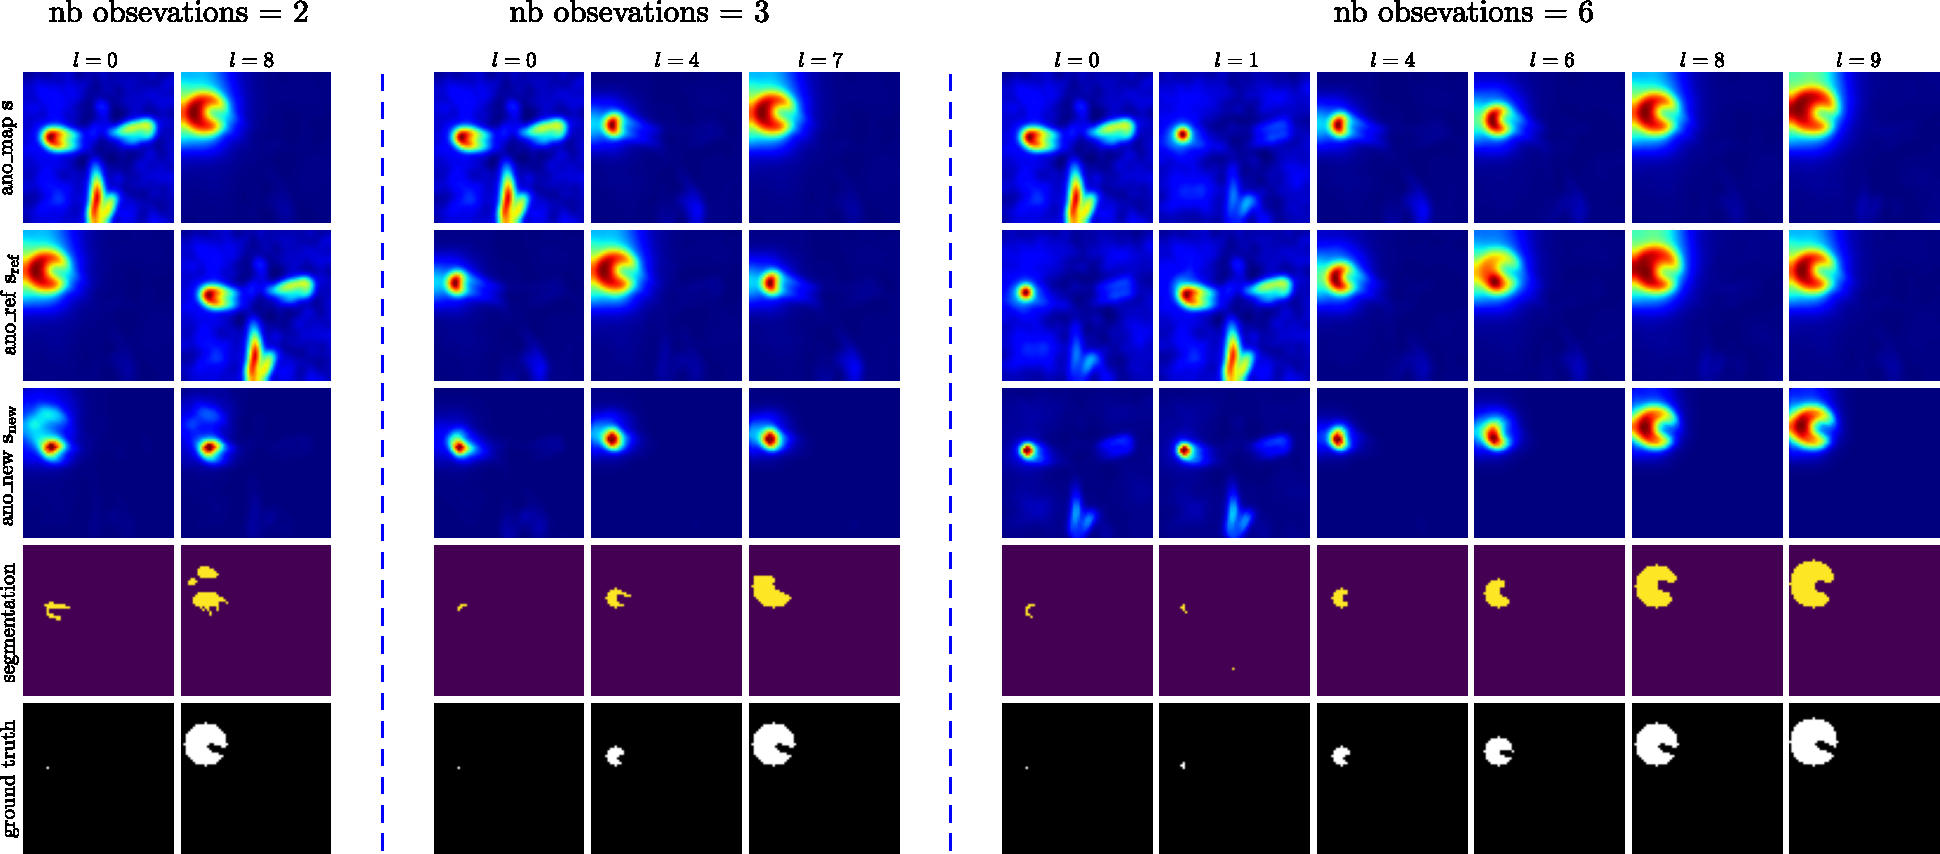
\includegraphics[width=\linewidth]{figures/lafm-vary-nb-fig.pdf}
    \caption{Effect of number of observations on output of LAFM.}
    \label{fig:lafm-vary-nb}   
\end{figure}

\subsection{Image anomaly score}
\label{sec:image-auprc-auroc}

Follow method discussed in \cref{sec:post-process}, we assign image level anomaly score as a summary operator of pixel level anomaly score map. We employ several common strategies, namely: 
\begin{itemize}
    \item \texttt{max}: use the maximum pixel score as image anomaly score. 
    \item \texttt{mean}: assign the average pixel scores as image anomaly score. 
    \item \texttt{mean-top$k$}: calculate the average of top $k$ pixel scores as image anomaly score. 
    \item \texttt{$q$-quantile}: calculate the average of top $q$th percentile pixel scores as image anomaly score. 
\end{itemize}

\cref{tab:auprc-auroc-image} reports the AUPRC and AUROC metrics for different methods and strategies. We apply each strategy to different pixel anomaly score maps that we have obtained so far. Pixel, FAM and LAFM refer to the original pixel residual map $D_p$, pixel anomaly map from FAM and LAFM, respectively. A key observation is that pixel residual error achieves the highest value for both AUROC and AUPRC at 97.5\% and 92.9\% respectively, while our proposed methods FAM only has performance around 86-90\%. We suggest that this may result from the application of several post-processing steps to $D_p$. FAM and LAFM are good for pixel segmentation, but also it neutralizes some information in the pixel residual map. For example, LAFM smooths the pixel anomaly map by concatenating information from other time points, which may reduce the contrast between healthy and anomalous images. 

% , specially FAM and LAFM operate patient wise, while AUPRC and AUROC metrics of image anomaly score is calculated dataset-wise. 
We also see that using max operator remains the best strategy to assign image anomaly score. On the other hand, mean operators have the worst performance, as it average all pixel scores. By doing so, it dilutes the anomaly information because most of our residual errors are small (background pixel). We can observe this effect clearly in mean-top-$k$ and mean-$q$-quantile methods, where the performance increases as we decrease the number of pixels that we consider. On the other hand, we see that LAFM has more stable performance than other methods. Even though mean operators still have lower performance, LAFM remains around 90\% AUROC and 85\%AUPRC, which is better than FAM or Pixel score. \cref{fig:auprc-auroc-curve-pixel} and \cref{fig:auprc-auroc-curve-lafm} show the AUPRC and AUROC curves using pixel distance $D_p$, and LAFM anomaly score, respectively. 

\begin{table}[htbp]
    \centering
    \begin{adjustbox}{max width=\textwidth}
        \begin{tabular}{lrrrrrr}
        \toprule
        & \multicolumn{3}{r}{AUPRC(\%)} & \multicolumn{3}{r}{AUROC(\%)} \\
        \cmidrule(lr){2-4} \cmidrule(lr){5-7}
        & FAM & LAFM & Pixel & FAM & LAFM & Pixel \\
        \midrule
        \texttt{max} & \textit{86.714} & \textit{92.074} & \textbf{92.889} & \textit{90.017} & \textit{96.589} & \textbf{97.509} \\
        \texttt{mean} & 23.558 & 74.778 & 62.905 & 35.604 & 83.692 & 77.458 \\
        \midrule
        \texttt{mean-top50} & 83.040 & 87.680 & 77.815 & 86.630 & 93.547 & 89.823 \\
        \texttt{mean-top100} & 79.827 & 86.380 & 73.208 & 83.723 & 92.484 & 86.521 \\
        \texttt{mean-top150} & 77.073 & 85.752 & 71.114 & 81.295 & 91.872 & 85.002 \\
        \texttt{mean-top200} & 74.347 & 85.266 & 70.011 & 79.067 & 91.422 & 84.242 \\
        \midrule
        \texttt{90.0-quantile} & 62.750 & 83.494 & 68.585 & 70.534 & 90.051 & 83.256 \\
        \texttt{92.5-quantile} & 68.351 & 84.307 & 69.030 & 74.536 & 90.662 & 83.593 \\
        \texttt{95.0-quantile} & 74.068 & 85.215 & 69.939 & 78.842 & 91.379 & 84.192 \\
        \texttt{97.5-quantile} & 79.660 & 86.336 & 73.036 & 83.572 & 92.442 & 86.398 \\
        \texttt{99.0-quantile} & 83.693 & 88.184 & 79.268 & 87.243 & 93.861 & 90.781 \\
        \bottomrule
        \end{tabular}
    \end{adjustbox}
    \caption[AUPRC and AUROC for image anomaly score]{AUPRC and AUROC for image anomaly score. \texttt{mean-top$k$} refers to taking the mean of the top $k$ the highest pixel anomaly scores. \texttt{$q$-quantile} refers to taking the mean of the pixel scores at the $q$th percentile. The best results for AUPRC and AUROC are highlighted in \textbf{bold}, calculated across all methods. Best results for each method are highlighted in \textit{italic}}
    \label{tab:auprc-auroc-image}
\end{table}

\begin{figure}[htbp]
    \centering
    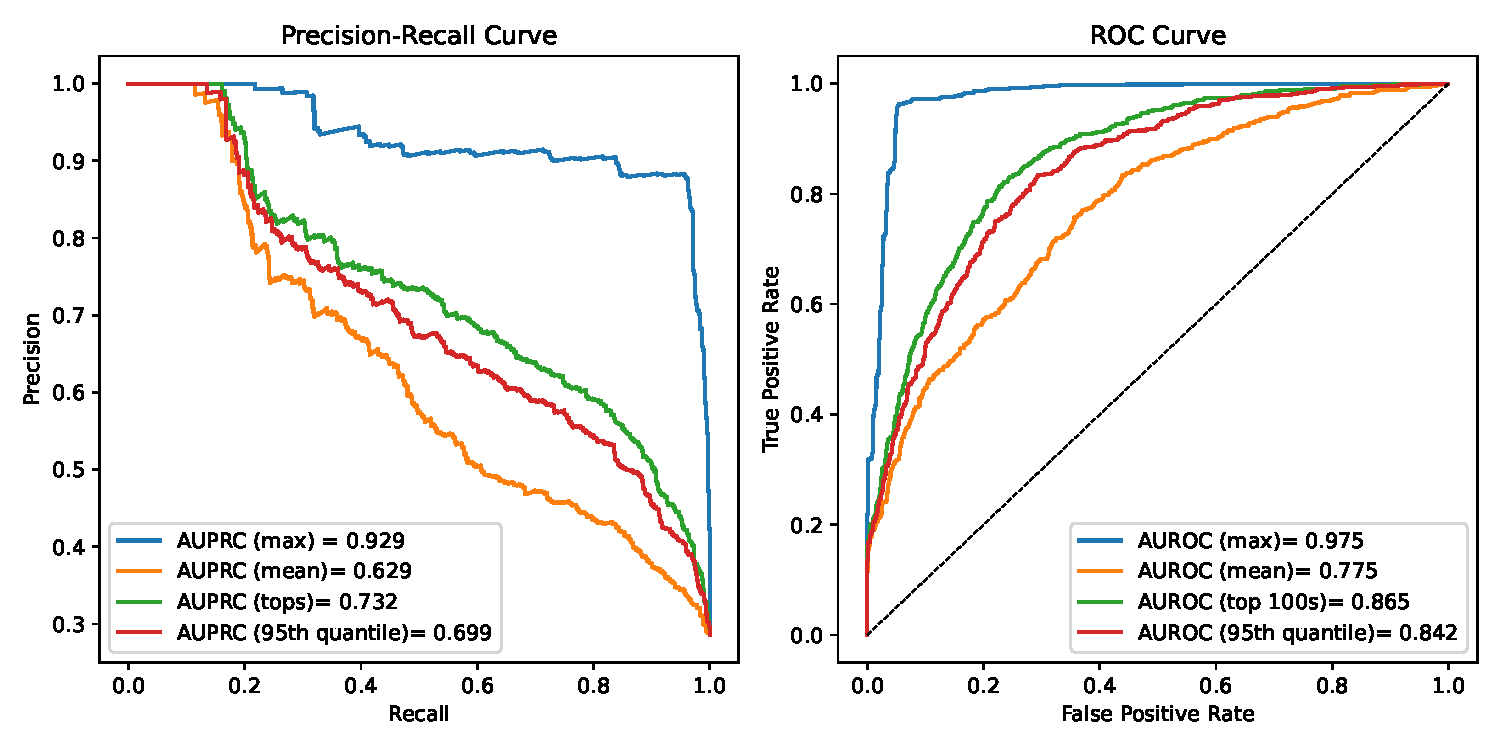
\includegraphics[width=0.8\linewidth]{figures/auprc-auroc-pixel.pdf}
    \caption[AUROC and AUPRC curves for image level score - Pixel distance]{AUROC and AUPRC curves for image anomaly score with different methods, apply to pixel distance $D_p$. Left: AUPRC curves. Right: AUROC curves.}
    \label{fig:auprc-auroc-curve-pixel}
\end{figure}

\begin{figure}[htbp]
    \centering
    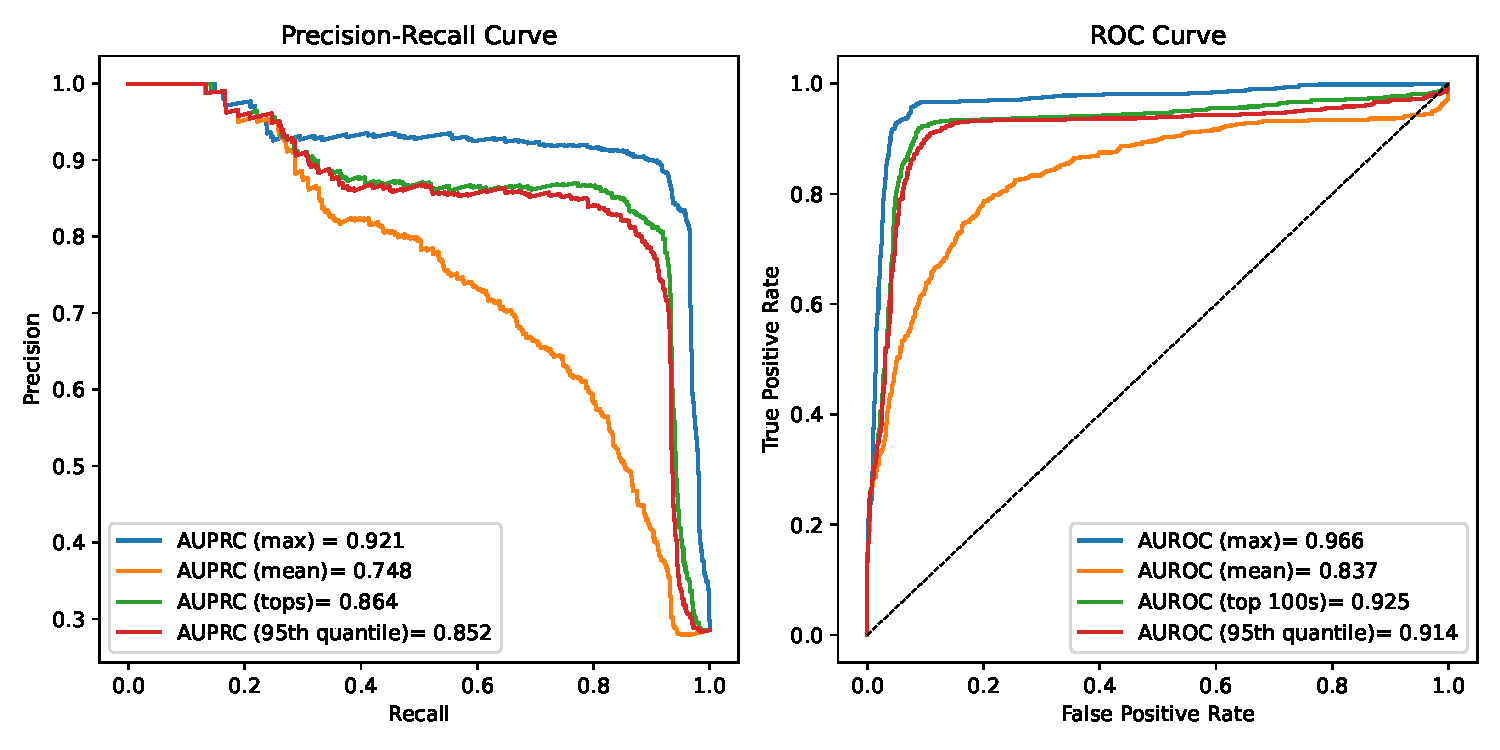
\includegraphics[width=0.8\linewidth]{figures/auprc-auroc-lafm.pdf}
    \caption[AUROC and AUPRC curves for image level score - LAFM score]{AUROC and AUPRC curves for image anomaly score with different methods, apply to LAFM anomaly score. Left: AUPRC curves. Right: AUROC curves.}
    \label{fig:auprc-auroc-curve-lafm}
\end{figure}



\chapter{Temporal Diffusion Model for data imputation}
\label{chap:tdm}

In this chapter, we introduce our implementation of temporal diffusion model for follow-up data generation. Our model is based on TADM model \cite{litricoTADMTemporallyAwareDiffusion2024}, which uses diffusion process to learn the residual growth of images in the temporal space. We cover the methodology in \cref{sec:TDM}. \cref{sec:tdm-implement} explains the implementation of our model, and \cref{sec:result-tdm} shows the results of our experiment. We also utilize \texttt{Starmen} dataset in this experiment.  

\minitoc

\section{Temporal Diffusion Model for follow up data generation}
\label{sec:TDM}

\begin{figure}
    \centering
    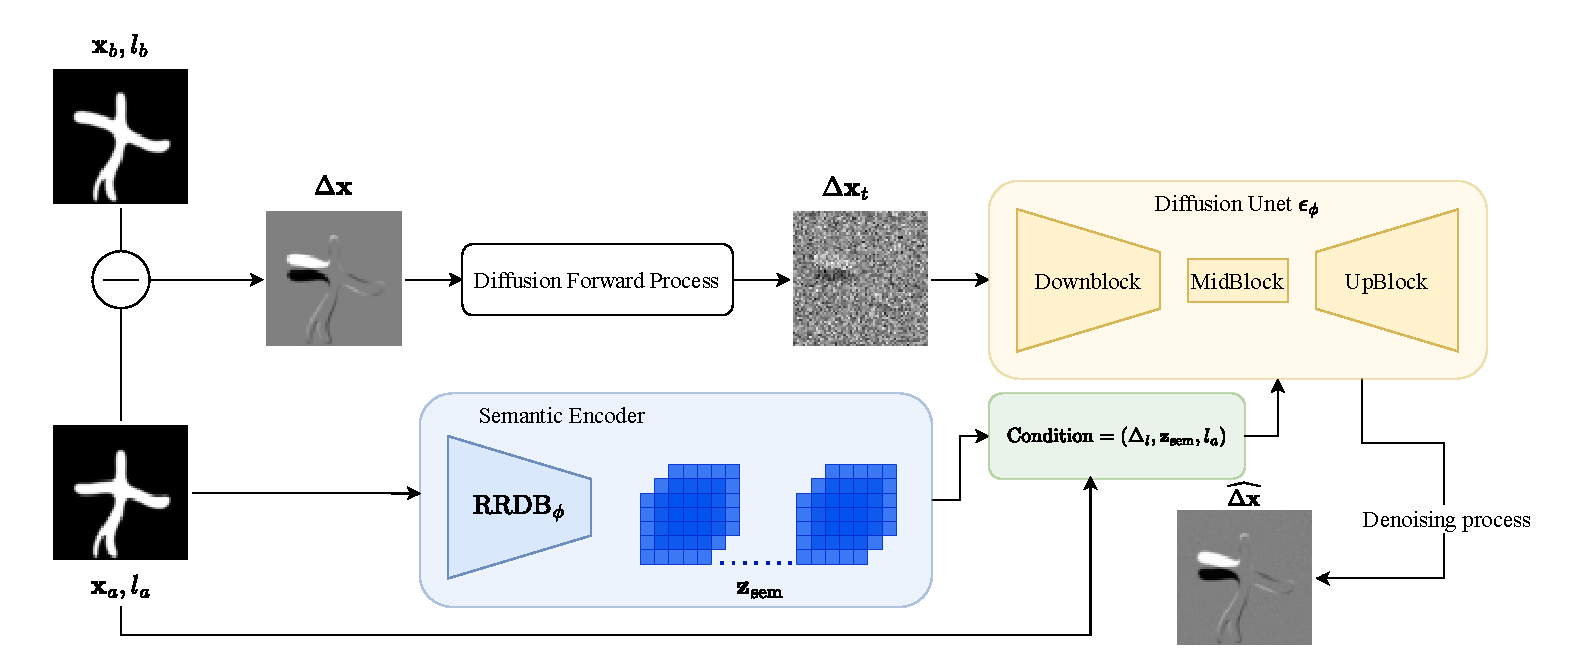
\includegraphics[width=1\linewidth]{figures/model-tdm.pdf}
    \caption[Overview of TDM framework]{Overview of our Temporal Diffusion Model (TDM). Our model takes as input the residual change $\Delta\rvx$ between 2 time points $l_a < l_b$, the conditions to the model are: the current baseline age $l_a$, a list of spatial representations extracted from RRDB \cite{zhang2018RRDB} encoder, the time interval $\Delta_l$. During \textbf{training}, the inputs go through normal diffusion forward-backward process and conditional UNet learns to predict the added noise. At \textbf{inference}, we sample a Gaussian random noise $\rvx_T \sim \mathcal{N}(0, \mathbf{I})$, use trained UNet to denoise with DDIM sampling scheme to predict the residual change. The target image is constructed by adding predicted residual to baseline image $\widehat{\rvx_b} = \rvx_a + \widehat{\Delta\rvx}$}
    \label{fig:model-tdm}
\end{figure}

In this section, we come back to our spatial-temporal setting and introduce our framework to use diffusion model to learn temporal dependencies between samples. As mentioned earlier, one major challenge in unsupervised anomaly detection in MRI scans is the presence of missing scans. Consequently, this raises the important task of imputing missing data based on the available observations. Consequentially, this raises an important domain of imputation of missing data, based on observation. We denote $\mathbf{X}^{\mathcal{O}}_{i} = \{\rvx_1, \rvx_2, \dots, \rvs_L\}$ as our set of observed data, and $\mathbf{X}^{\mathcal{M}}_{i} = \{\rvx_1, \rvx_2, \dots, \rvs_M\}$ the set of missing data that we want to impute, for a patient $i$. Since both training and inference are performed on a per-patient basis, we drop the subscript $i$ for brevity. Our problem setting for temporal diffusion model becomes to learn the conditional distribution of $p(\rvx_m | \rvx_l)$ with $m \in [1 \dots M]$ and $l \in [1 \dots L]$. Our model operates as an autoregressive model that sequentially reconstructs the follow up sample from the previous one, so we have $m < l$. We note that $m$ and $l$ do not need to be consecutive, so $(l - m) \geq 1$.

% We note that the ideal situation would be to learn the joint distribution of all missing data at once, conditioned on all observed data. 

To characterize temporal features within sequences, we adopt the implementation of Temporal-Aware Diffusion Model (TADM) \cite{litricoTADMTemporallyAwareDiffusion2024}. Compared to other existing SOTA models, TADM offers several advantages: 
\begin{itemize}
    \item It provides more flexibility than approaches based on interpolation (\cite{lozuponeLDAE2025}), which requires two input images to be able to generate (interpolate) missing images in between. On the other hand, TADM has the capacity of generating follow up image in any time point in the future based on current image. 
    \item Instead of learning the whole age-related changes within the image, TADM is trained by learning the residual changes between 2 time points. This reduces the complexity of the problem, and minimize the generation errors. 
    \item Consequently, TADM conditions the model on the age gap between the input and output scans rather than directly on the output age. The authors argue that because the same age gap can happen between scans acquired at difference ages, conditioning on age gap avoids the necessity of including samples from every age group in the training set. This is particularly beneficial when the dataset has limited samples in some age groups \cite{litricoTADMTemporallyAwareDiffusion2024}.
\end{itemize}

By combining age gaps (time interval) and residual changes (spatial difference), TADM is trained to learn the distribution of temporal progression. During training, we use pairs of images denoted as $\rvx_a$ and $\rvx_b$, acquired from the same patient at two different time points $l_a < l_b$. These scans are used to compute the residual change $\Delta\rvx = \rvx_b - \rvx_a$, which represents the image growth over the interval $\Delta_l = l_b - l_a$. TADM takes $\Delta\rvx$ and $\Delta_l$ as input and undergoes the standard forward–backward diffusion process to learn the underlying distribution $p(\Delta\rvx \mid \Delta_l)$. At inference, by performing the denoising process, we can sample $\widehat{\Delta\rvx}$ given a baseline age $l_a$ and time interval $\Delta_l$. The future image at $l_b$ is then predicted as $\widehat{\rvx_b} = \rvx_a + \widehat{\Delta\rvx}$. \cref{fig:model-tdm} shows an overview of our TDM framework. 

One major concern with this approach is that different patients may exhibit different rates of change over the same time interval. To account for this, TDM also employs an encoder to extract a non-spatial representation of the input, which is then used as a conditional signal to guide the diffusion process. We make the underlying assumption that the current image contains the most meaningful information about a patient’s state up to this point. In other words, the sequence of images can be viewed as a Markov chain, where future images depend only on the previous one. In addition, we also condition the diffusion process on baseline age $l_a$, under the assumption that the rate of change varies across different ages. Following \cite{litricoTADMTemporallyAwareDiffusion2024}, our TDM comprises two blocks: i) an encoder to extract semantic representation of baseline image, and ii) an UNet block as diffusion model to predict the noises added. Our TDM differs from TADM in that TADM employs an additional Brain Age Estimation (BAE) module to predict the age gap between the predicted image $\widehat{\rvx_b}$ and the baseline $\rvx_a$. It then incorporates the difference between the predicted age gap, $\widehat{\Delta_l} = BAE(\widehat{\rvx_b}, \rvx_a)$, and the true age gap $\Delta_l$ into its loss function. Conceptually, this can be interpreted as an adversarial loss, similar to that used in \ac{GAN} models. This requires additional step of pretraining the BAE module, and we omit it in our experiment for simplicity. Our denoising U-Net is also a conditional diffusion model that follows the same methodology as SDM. For the semantic encoder, we employ the Residual-in-Residual Dense Blocks (RRDB) module \cite{zhang2018RRDB}. Unlike the semantic encoder in SDM (ResNet50), RRDB outputs a list of spatial representations of the input, denoted as $\rvz_{\text{sem}, i} \in \mathbb{R}^{h \times w}$, corresponding to the $i$-th block of the RRDB.
\begin{description}
    \item[Training]: during diffusion step, TDM is trained to predict the noise $\epsilon$ added to the input $\Delta_l$ at time step $t$. The loss function from \cref{eq:loss-ddpm} is updated to incorporate patient specific data as follows: 
    \begin{equation}
    \label{eq:loss-tdm}
        \begin{aligned}
        \mathcal{L} (\theta, \omega) &= ||\epsilon - \epsilon_{\theta} (\Delta\rvx_t, t; \Delta_l, l_a, \mathbf{Z}_a ||^2 \\
        \mathbf{Z}_a &= \mathrm{Enc_{\omega}}(\rvx_a))
        \end{aligned}
    \end{equation}
    where $\Delta\rvx_t = \sqrt{\bar\alpha} \Delta\rvx_0 + \sqrt{\bar\alpha_t} \epsilon$ (\cref{eq:xt-from-x0}), $t \sim \mathrm{Unif}[1, T]$ is the time step, $z_a$ is latent representation of baseline image from RRDB encoder. Similar to our spatial diffusion model, parameters of UNet and Encoder, $\theta$ and $\omega$ respectively, are jointly trained through backpropagation. 
    
    \item[Inference]: our model impute missing scans by an autoregressive process. Given a sequence of observed data $\mathbf{X}^{\mathcal{O}}_{i} = \{\rvx_1, \rvx_2, \dots, \rvs_L\}$, we impute the missing image at time $m$ by finding the closest image from the observed set $\rvx_l \in \mathbf{X}^{\mathcal{O}}$ such that $l < m$. Our model takes as inputs baseline image $\rvx_a$ and time interval with respect to baseline time $\Delta_l = m -l$. The reverse process starts from random Gaussian noise $\Delta_T \sim \mathcal{N}(0; \mathbf{I})$ and progressively denoises through $\epsilon_{\theta}(\Delta_T, t; \rvx_a, \Delta_l, z_a)$. The predicted residual change $\widehat{\Delta_l}$ is then added to baseline image to generate missing image $\widehat{\rvx_m} = \rvx_a + \widehat{\Delta_l}$. 
\end{description}

\section{TDM implementation}
\label{sec:tdm-implement}

\paragraph{UNet}: Our temporal diffusion model is modified from TADM implementation \cite{litricoTADMTemporallyAwareDiffusion2024} \footnote{Available at \href{https://github.com/MattiaLitrico/TADM-Temporally-Aware-Diffusion-Model-for-Neurodegenerative-Progression-on-Brain-MRI}{https://github.com/MattiaLitrico/TADM-Temporally-Aware-Diffusion-Model-for-Neurodegenerative-Progression-on-Brain-MRI}}. Similar to base diffusion model, our UNet comprises input blocks (with downsampling layer), a middle block, and out blocks (with upsampling layer) which are the symmetric counterparts of corresponding downsampling blocks. Down and Up blocks contain 4 levels with channel multipliers of $[32, 64, 128, 256]$. Unlike SDM model, each level in TDM has 2 residual blocks (ResBlock), followed by downsampling (upsampling) block. We omit cross-attention layers in the TDM, as the model operates on residual changes $\Delta \rvx$ rather than the original image $\rvx$, where spatial information is less prominent. This is similar to the implementation from TADM paper. 
\paragraph{Condition signals}: similar to SDM, time step condition $t$ is embedded using sinusoidal embeddings. The condition dimension is $d_{cond} = 32$. For semantic encoder, we use RRDB \cite{zhang2018RRDB} as our backbone network, with 8 blocks and each block has 64 channels. The RRDB is not initialized but is trained from scratch jointly with UNet module. Other patient-specific data, such as age $l_a$ and age difference $\Delta l$, are projected using a linear layer to match the dimension of the time embedding vector. Unlike the SDM, all conditions are injected into the ResBlocks by being summarized with the model’s hidden state. We note that all conditions (except semantic encoded $z_a$) are represented as vectors, while the hidden states are spatial representations produced by Conv2D layers. Therefore, the summation is performed via broadcasting. Formally we have $h := h + \psi_1(t) + \psi_2(l_a) + \psi_3(\Delta_l) + z_{a}$, with $\psi_1, \psi_2, \psi_3$ are trainable projection layers applied to time step, age and time interval, respectively. 
\paragraph{Training configuration}: TDM is trained with 500 epochs, using Adam optimizer with learning rate $2.5 \times 10^{-4}$. Similar to SDM, we employ EMA strategy to smooth out parameters, with EMA decay rate is $0.9999$ and EMA is updated after every 10 batches. \cref{tab:tdm-config} shows the details configurations of our TDM network.

\begin{table}[h]
\captionsetup{justification=raggedright,singlelinecheck=false}
\caption{Temporal Diffusion Model (TDM): configurations and parameters}
% \resizebox{\columnwidth}{!}{%
\begin{tabular}{ll}
\toprule
\multicolumn{2}{l}{\textbf{Encoder $\mathrm{Enc}_{\omega}$}} \\
\midrule
Backbone & \texttt{RRDB} \cite{zhang2018RRDB} \\
Input Modality & $1 \times 64 \times 64 $ \\
RRDB number of blocks & 8 \\
RRDB number of features & 64 \\
\midrule
\multicolumn{2}{l}{\textbf{Diffusion UNet $\epsilon_{\theta}$}} \\
\midrule
Input Shape & $(B, 1, 64, 64)$, with batch size first \\
Channels multipliers & [32, 64, 128, 256] \\
Residual Blocks per Level & 2 \\
Conditional injection & Summarize \\
Dropout & 0.1 \\
Time embedded dimension & $d_{cond} = 32$ \\
Timestep & 1000 \\
Beta Schedule & Linear, $\beta_t \in [10^{-4}, 2 \times 10^{-2}]$ \\
\midrule
\multicolumn{2}{l}{\textbf{Training Configuration}} \\
\midrule
Optimizer & Adam \\
Learning Rate & $2.5 \times 10^{-4}$ \\
EMA Decay & 0.999 \\
Train Batch Size (effective) & 20 \\
Training Duration & 500 epochs / $\sim$4.5 hours \\
Hardware & 1 x Nvidia L40S (45 GiB) \\
\bottomrule
\end{tabular}
% }
\label{tab:tdm-config}
\end{table}

\section{Results}
\label{sec:result-tdm}

In this section, we present our results on using a temporal diffusion model to impute missing data. We demonstrate how the model leverages temporal information from previous observations to generate accurate predictions for the missing values, and we analyze its performance across different scenarios.

% \subsubsection{Imputing missing data}
% \label{sec:result-tdm-recon-error}

\subsection{Imputing subsequence images}
First, we test the reconstruction performance of \ac{TDM} in case of predicting images using information from preceding images. In this simple case, the time interval is $\Delta_l \sim 1$. \cref{tab:tadm-error-previous} shows the similarity metrics and residual errors of subsequently imputation for different anomaly types. We see that \ac{TDM} achieves the best performance on the \texttt{healthy} dataset, which is expected since, during training, our model only sees normal samples. When \ac{TDM} encounters anomalous images during inference, even though semantic representations are provided by the RRDB semantic encoder, our model does not know how to process this information and fails to predict how the anomaly will progress over time. Not only that, but the presence of an anomaly distorts the normal semantic representation, causing our model to produce lower-quality follow-up images. This can be observed in \cref{fig:tadm-impute-gcircle}. Starting from the 2\textsuperscript{nd} observation (5\textsuperscript{th} time point), the anomaly is present, causing subsequent imputations to deteriorate in quality. The anomaly does not grow but rather remains blurry in the following time points.

For healthy dataset, we see that \ac{TDM} achieves very high results, both in terms of similarity metrics and residual errors, with MSSIM closed to 100\%, and LPIPS is around $26 \times 10^{-3}$. 

\begin{table}[htbp]
    \centering
    \begin{adjustbox}{max width=\textwidth}
    \begin{tabular}{lrrrrrr}
    \toprule
    & \multicolumn{4}{c}{Similarity metrics} & \multicolumn{2}{c}{Residual errors} \\
    \cmidrule(lr){2-5} \cmidrule(lr){6-7}
    & SSIM \textuparrow & MSSIM \textuparrow & PSNR \textuparrow & LPIPS (e-3) \textdownarrow & $l1$-error(e-3) \textdownarrow & $l2$-error(e-3) \textdownarrow \\
    \midrule
    \texttt{healthy} & 77.26 & 99.17 & 37.40 & 26.61 & 9.90 & 0.19 \\
    \texttt{growing\_circle} & 75.02 & 97.72 & 23.97 & 33.70 & 17.77 & 6.31 \\
    \texttt{darker\_circle} & 76.68 & 99.07 & 33.05 & 29.19 & 10.99 & 0.52 \\
    \texttt{darker\_line} & 75.82 & 98.90 & 31.73 & 29.31 & 11.60 & 0.71 \\
    \bottomrule
    \end{tabular}
    \end{adjustbox}
    \caption[TDM imputation error - use previous image]{Imputation error: using the previous image to predict the next consecutive image. Results are reported for each type of anomaly.}
    \label{tab:tadm-error-previous}
\end{table}

\subsection{Imputation with random time interval}

\begin{figure}[htbp]
    \centering
    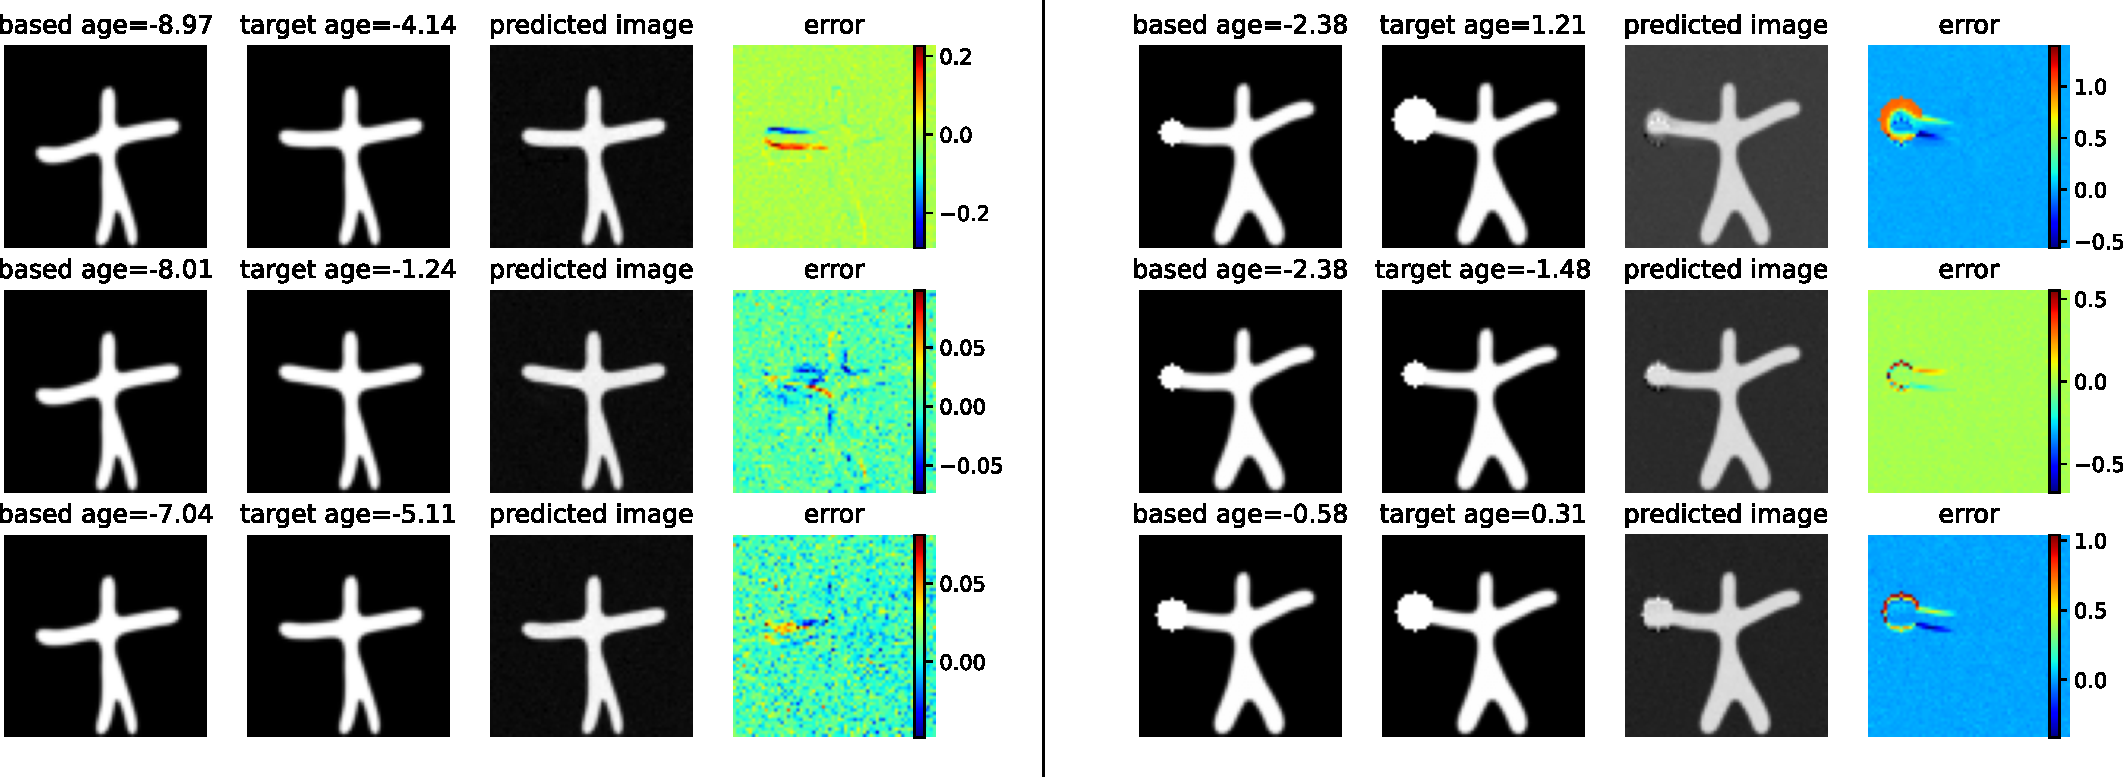
\includegraphics[width=0.8\linewidth]{figures/tadm-randompair.pdf}
    \caption[Example of imputation from TDM - random time interval]{Example of imputation with random time interval. Left: healthy sample. Right: anomaly sample. For each image, from left to right: current image, future image, predicted image, and residual error ($l1$-error)}
    \label{fig:tadm-randompair}
\end{figure}

Next, we test the model capacity of generating follow-up data at arbitrarily $\Delta_l$ time steps in the future. \cref{tab:tadm-error-randompair} reports reconstruction errors for healthy dataset. Results are reported as average of different time gap group. Gap bin $(0-1)$ corresponds to our previous case: imputing subsequence data. We clearly see that the quality decreases as time gap increases, for both similarity metrics and pixel residual errors. The only exception is LPIPS metrics, where we see the best result is obtained at time point really far into the future (time gap bin $(10-11)$), although the differences is small compared to case of subsequent imputation. 

This result can be explained by the fact that the residual growth between 2 consecutive time points is relatively smaller. So even though our model is trained with all random pairs of images (thus it is trained with all time differences), its performance is best when we use preceding image as input conditions. \cref{fig:tadm-randompair} shows examples of generating follow-up images with different time gap. 

\begin{table}[htbp]
    \centering
    \begin{adjustbox}{max width=\textwidth}
    \begin{tabular}{lrrrrrr}
    \toprule
    & \multicolumn{4}{c}{Similarity metrics} & \multicolumn{2}{c}{Residual errors} \\
    \cmidrule(lr){2-5} \cmidrule(lr){6-7}
    $\Delta_l$ gap group & SSIM \textuparrow & MSSIM \textuparrow & PSNR \textuparrow & LPIPS (e-3) \textdownarrow & $l1$-error(e-3) \textdownarrow & $l2$-error(e-3) \textdownarrow \\
    \midrule
    0-1 & \textbf{84.882} & \textbf{99.158} & \textbf{38.266} & 25.867 & \textbf{9.001} & \textbf{0.151} \\
    1-2 & 83.955 & 99.118 & 36.778 & 26.513 & 9.769 & 0.226 \\
    2-3 & 83.422 & 99.037 & 34.670 & 28.398 & 10.835 & 0.362 \\
    3-4 & 84.150 & 98.921 & 32.524 & 28.877 & 11.828 & 0.630 \\
    4-5 & 83.235 & 98.826 & 31.843 & 29.618 & 12.453 & 0.774 \\
    5-6 & 82.772 & 98.744 & 30.906 & 31.476 & 13.255 & 0.898 \\
    6-7 & 83.273 & 98.635 & 30.372 & 31.266 & 14.002 & 1.040 \\
    7-8 & 82.625 & 98.532 & 29.580 & 32.333 & 14.432 & 1.215 \\
    8-9 & 83.880 & 98.564 & 29.427 & 29.821 & 14.433 & 1.289 \\
    9-10 & 83.127 & 98.507 & 29.099 & 27.434 & 15.178 & 1.440 \\
    10-11 & 83.329 & 98.473 & 28.870 & \textbf{25.325} & 15.436 & 1.372 \\
    11-12 & 76.029 & 98.373 & 26.884 & 29.327 & 17.134 & 2.078 \\
    \bottomrule
    \end{tabular}
    \end{adjustbox}
    \caption[TDM imputation error - use random time interval]{Imputation errors: using random pairs with different time interval. Results are reported as the average for each time gap group. Best results are highlighted in \textbf{bold}}
    \label{tab:tadm-error-randompair}
\end{table}

% \paragraph{Imputation of sequence}
\cref{fig:tadm-impute-error} shows examples of imputing all missing images based on observed data. TDM generates images in an autoregressive process. Starting from an observed time point, the model predicts the next succeeding image, and this newly generated image becomes the baseline for the following prediction. The process continues until the next observed time point. 

\begin{figure}[htbp]
    \centering
    \begin{subfigure}{0.68\textwidth}
        \centering
        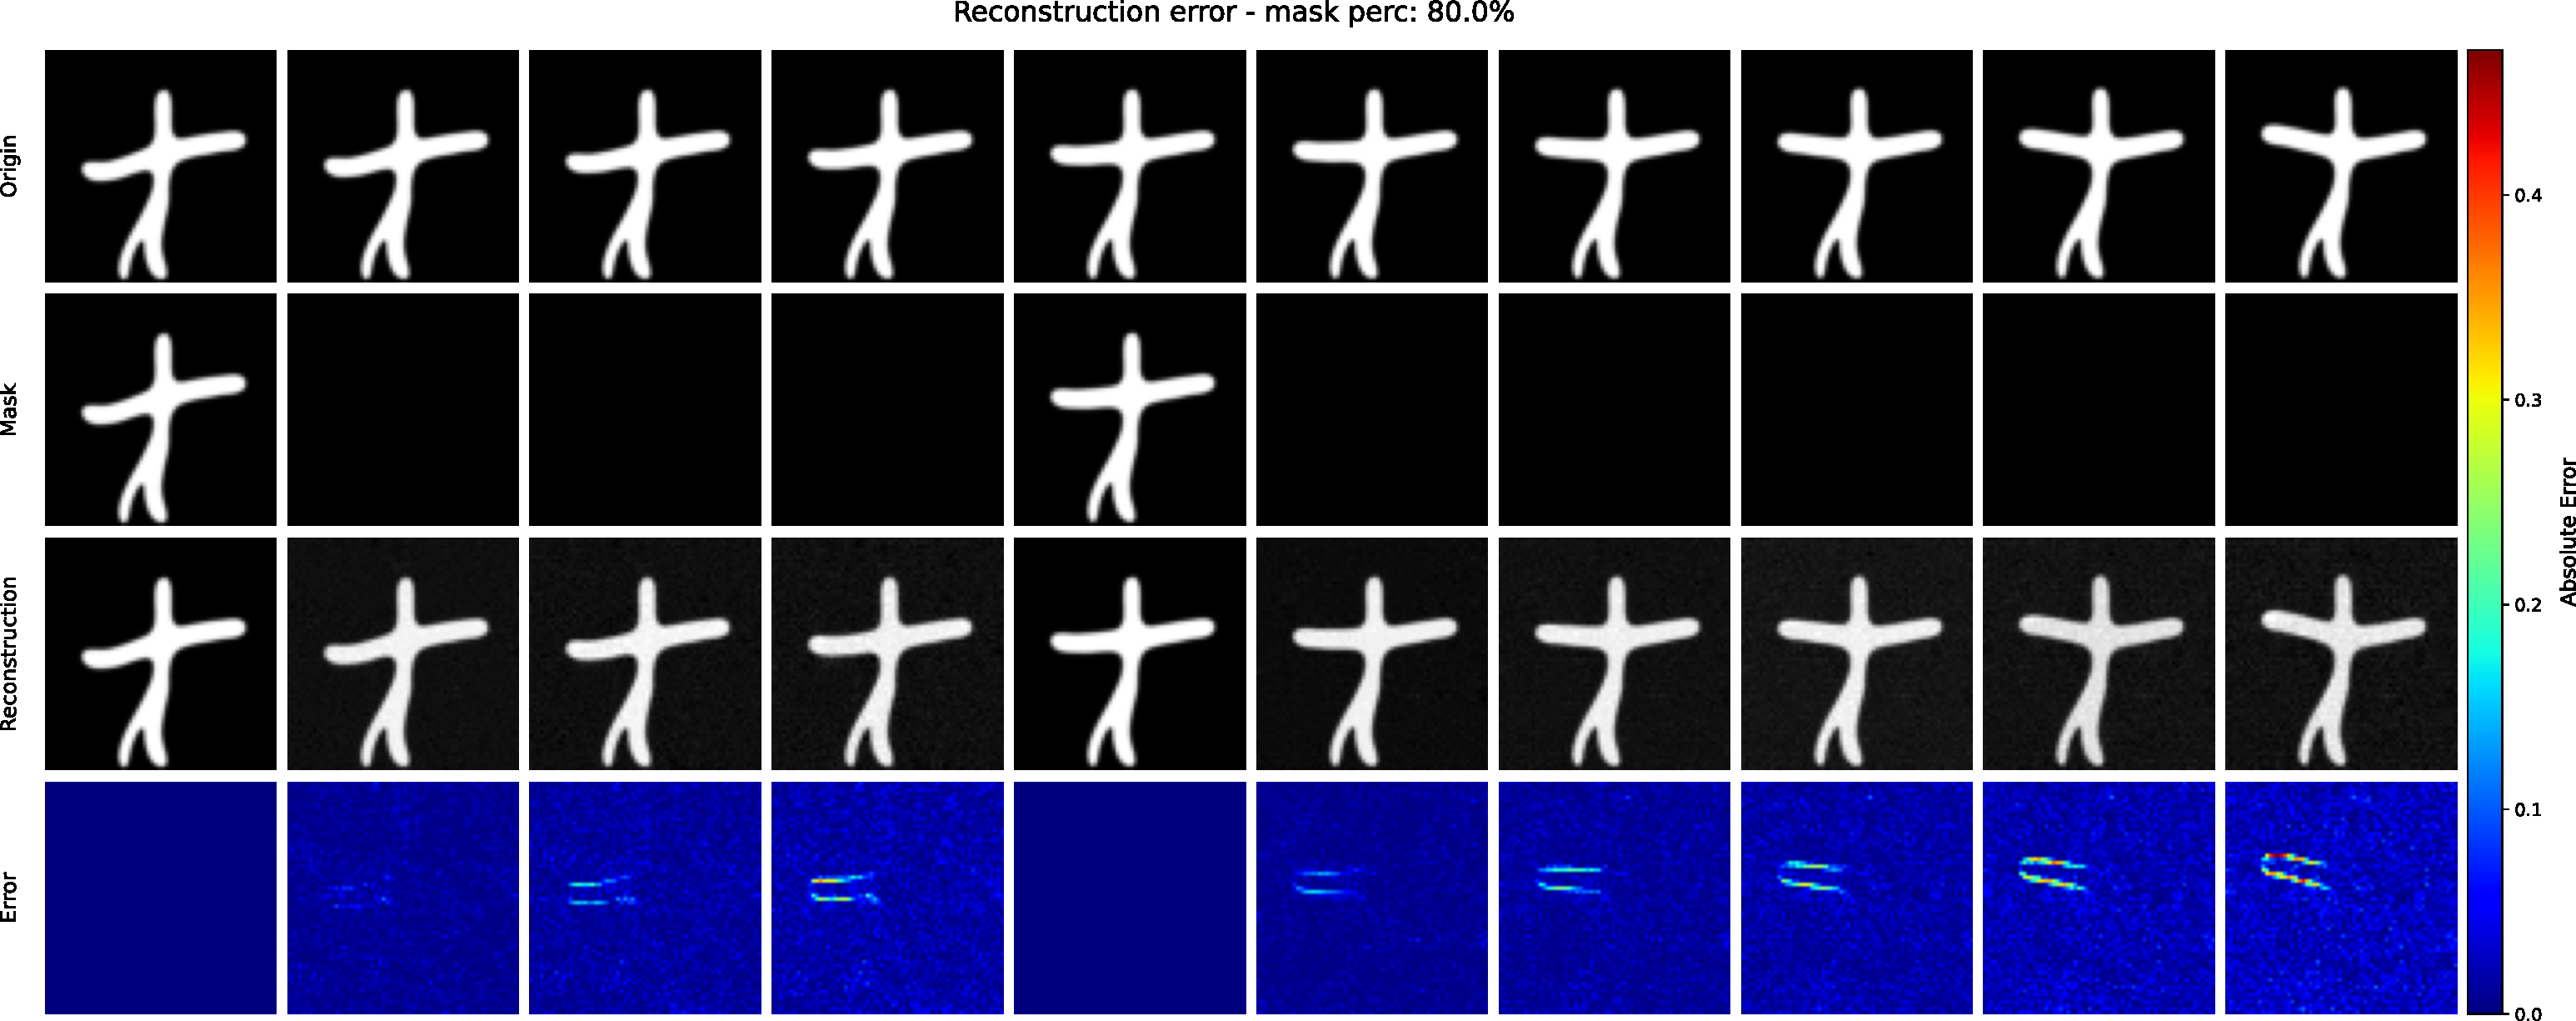
\includegraphics[width=1.0\linewidth]{figures/tadm-impute-healthy.pdf}
        \caption{Imputation for healthy subject.}
        \label{fig:tadm-impute-healthy}
    \end{subfigure}
    \hfill
    \begin{subfigure}{0.68\textwidth}
        \centering
        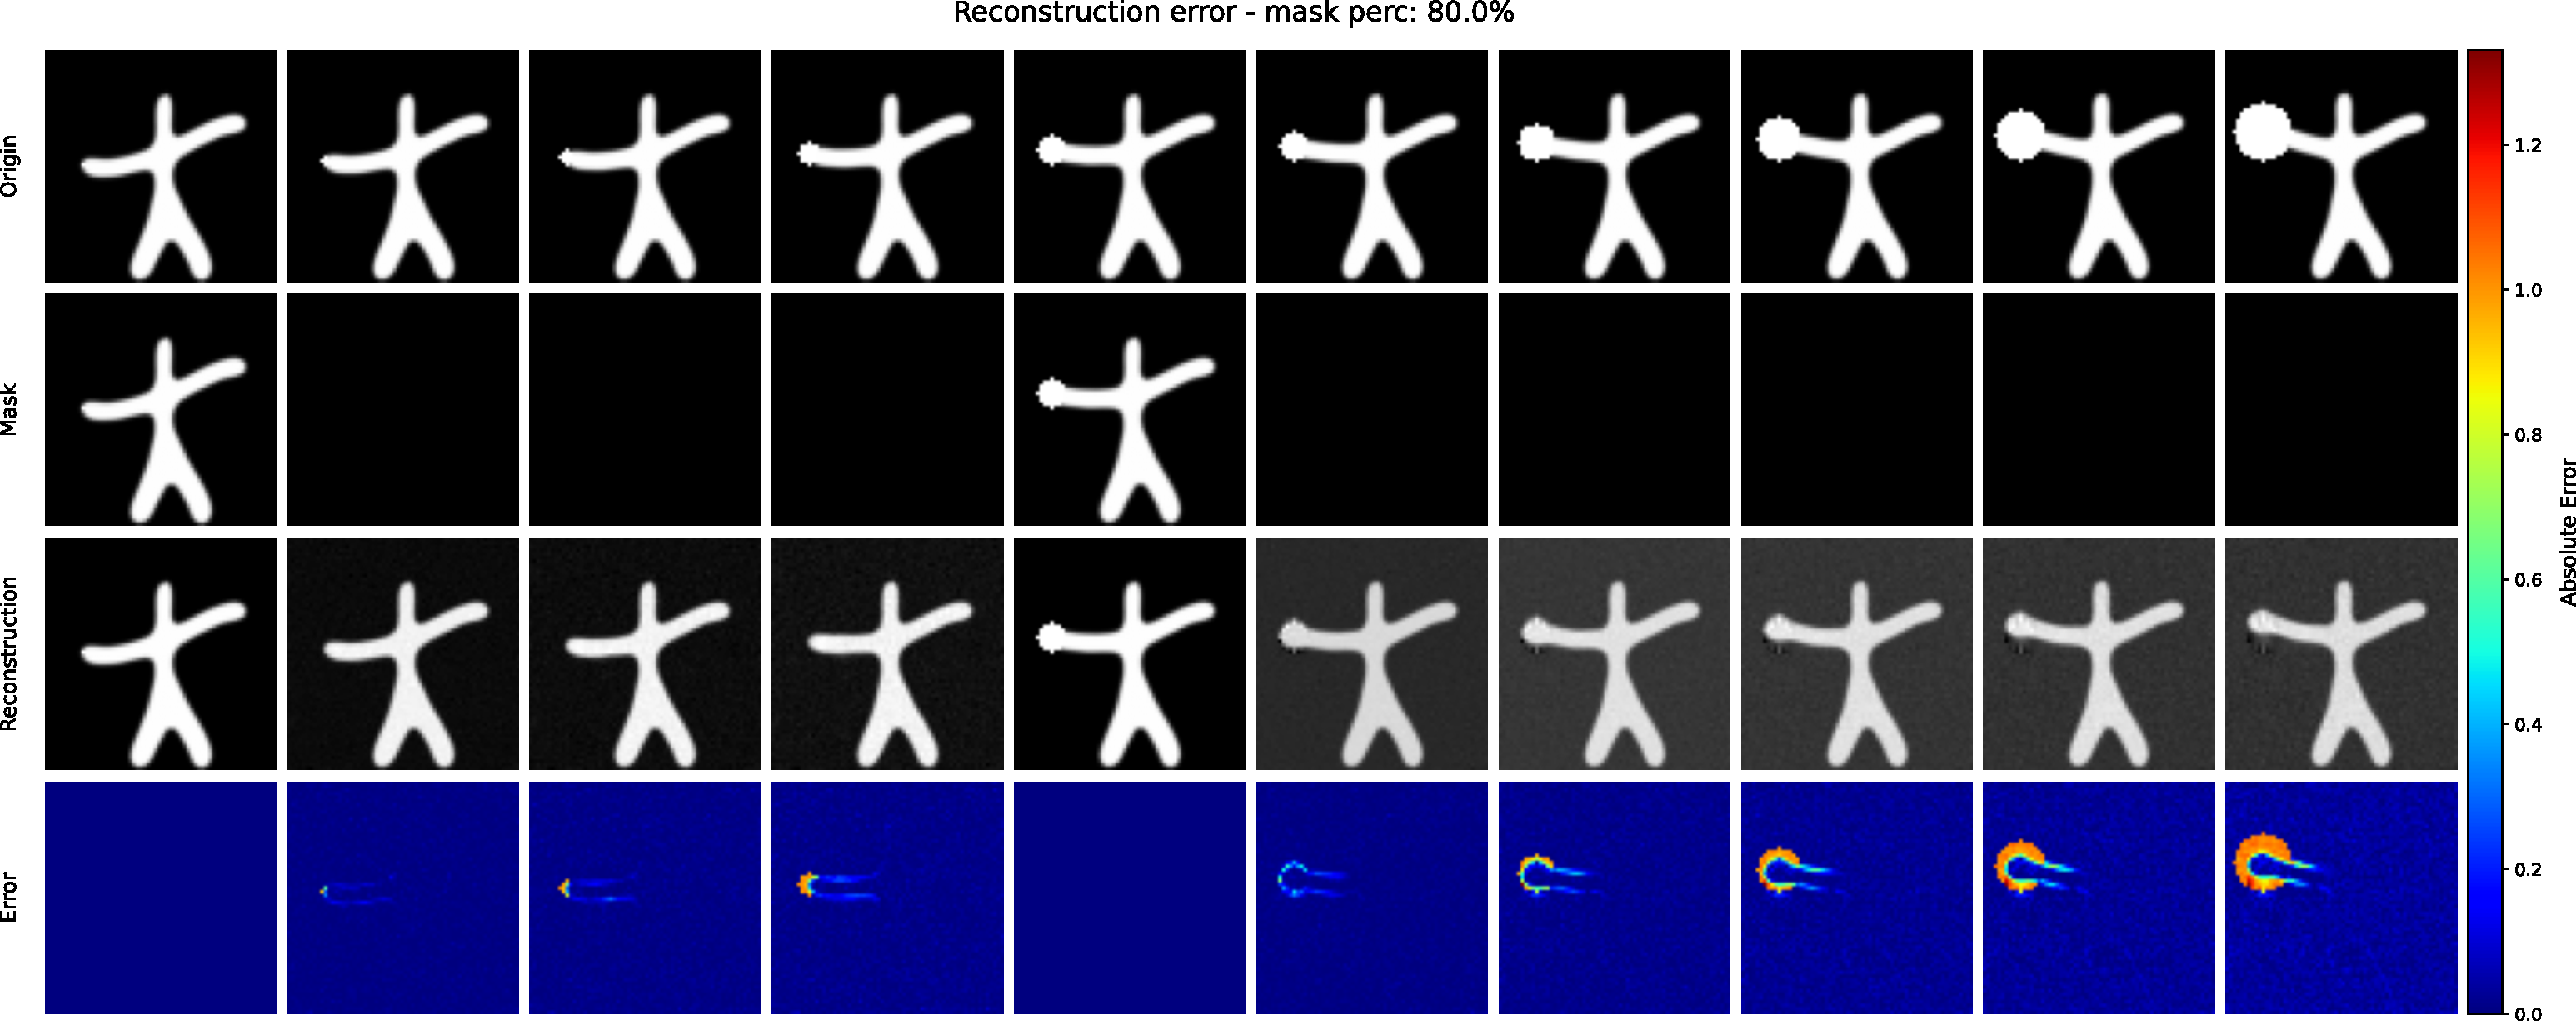
\includegraphics[width=1.0\linewidth]{figures/tadm-impute-gcircle.pdf}
        \caption{Imputation for anomaly subject.}
        \label{fig:tadm-impute-gcircle}
    \end{subfigure}
    \caption[Example imputation of missing data sequences using TDM]{Example of imputing missing data from TADM model. \cref{fig:tadm-impute-healthy} shows example from healthy subject, \cref{fig:tadm-impute-gcircle} shows example for anomaly subject. From top to bottom of each image: original data, masked observed data, imputed data sequence, $l1$-error.}
    \label{fig:tadm-impute-error}
\end{figure}

\subsection{Oversampling}

To test the model capacity to generate new samples that follow the same trajectory of observed data, we oversample by using the last observation as condition and generate a number of follow-up images with time interval $\Delta_l = 1$. \cref{fig:tadm-oversample} shows an example of oversampling for healthy subject. All generated images here are completely new and not included in our dataset. From the residual error (compared to the last observation), we see that our model efficiently learn to recognize the moving part of the sequence (the left hand). For each image in the subsequence, it gradually moves this part higher to align with the subject's trajectory.

\begin{figure}[htbp]
    \centering
    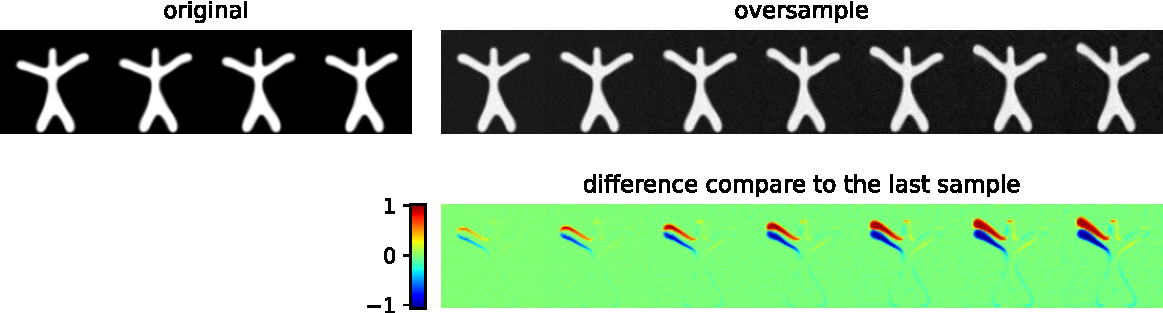
\includegraphics[width=0.75\linewidth]{figures/tadm-oversample.pdf}
    \caption{Example of oversampling with TDM.}
    \label{fig:tadm-oversample}
\end{figure}

\chapter{Conclusion}
\label{chapter:conclusion}

\section{Summary}

In this internship project, we studied the application of diffusion models for \ac{UAD}, both in spatial and temporal contexts. Building on recent developments in diffusion models, we investigated the feasibility of addressing some of their critical limitations. First, we aimed to improve reconstruction quality by developing a mechanism that effectively conditions the diffusion process on the input image. To achieve this, we used a semantic encoder to extract a rich representation of the input, which is injected into our model using shift and scale operators. The benefits of our method are twofold. First, by avoiding direct concatenation of the input, we reduce the risk of data leakage, thereby preventing the model from simply memorizing the answer. Second, by employing the AdapGN mechanism, our model remains simpler than alternatives that rely on attention mechanisms or input concatenation. Finally, by choosing an appropriate noise level, our approach can correct anomalous regions while preserving the high-quality structure of healthy areas.

Next, we improved the performance of anomaly segmentation. Specially we focused on how to reduce false positive, which is a big challenge of reconstruction-based UAD methods. We demonstrated that classic quantile methods are not sufficient to deal with subtle anomalies, and their performance highly depends on the composition of the dataset. We introduced two modules: the feature attention module (FAM) and Longitudinal attention fusion module (LAFM) that align with \ac{UAD} principles: (i) they do not require labeled or ground truth train dataset to perform greedy search for best threshold, and (ii) they are robust to different data compositions. FAM is presented to incorporate structural similarities to eliminate residual error caused by model error. Additionally, LAFM leverages temporal information from multiple time points to further smooth the residual maps. LAFM accounts for the temporal persistence of anomalies, enabling the detection of subtle anomalies at earlier stages, under the assumption that they will also be present in future observations. Our model shows promising results and outperforms all previous quantile methods. Furthermore, both FAM and LAFM exhibit more stable performance across datasets with varying proportions of healthy and anomalous samples.

For longitudinal learning, we presented a temporal diffusion model and its capacities to generate future images based on current observed data. Even though we did not exploit TDM in the context of anomaly detection, our model effectively captures the residual progression of healthy patients across arbitrary time intervals. This validates the ability of diffusion models to learn longitudinal progression, and it serves as an immediate step for future development. 

\section{Limitation and future work}
\label{sec:limitation}

Despite showing promising result, our approach has certain limitations that can be improved in future work. First, our proposed fusion modules (FAM and LAFM) do not form a unified framework. Instead, their performance varies across different test cases and metrics. For example, FAM outperforms the other in reducing false positive segmentation, while LAFM is more effective in accurately segmenting true anomaly. In the case of image wise anomaly score, results suggests that raw pixel distance with automatic Yen threshold is the most effective strategy. We can switch between them to achieve optimal results, or use one as an initial mask for other, but it introduces more complexity into the post processing pipeline. Furthermore, our model is heavily curated for our synthetic dataset, which may introduce bias and risk of overfitting. More extensive evaluation is needed to assess the generalization capabilities of our model.

A key aspect we wish to emphasize is the spatio-temporal modeling, as it is the main target of our project. Even though we utilize temporal information to increase accuracy, we note that this functions more as a filtering/smoothing operation than as a statistical model. While our approach offers the benefit of training free (LAF module), it has major limitation in capturing temporal variability (population level) and spatial inter-variability (personal level). It is important to note that, in our model, each patient is processed independently, and we do not make use of shared information between patients. Our project is inspired by LVAE model of Sauty et al. \cite{SautyLongitudinalVAE2022}, in which they successfully impose mix effect model on the latent space of standard \ac{VAE}. By combining longitudinal learning with generative learning, LVAE offers a more powerful solution for progression modeling. One notable example is that LVAE can propagate both to the past or future, while our TDM can only generate future images. Also, LVAE operates similarly to a Gaussian process, it makes use of all available data to impute missing data, but our model currently can only take the most recent image as condition. We aim to apply the same principle of LVAE to diffusion model. There are other models motivated by the same principle. Chen et al. \cite{chenOrthogonalMixedEffectsModelingLongitudinal} use orthogonal linear transformation to disentangle global and individual trajectory, also apply to \ac{VAE} model. \cite{ca23LongitudinalNormalizingFlow} use normalizing flow to model temporal dependencies. The main challenge for such adaptation is that in \ac{VAE}, each sample corresponds to only one (normally non-spatial, low dimension) latent variable, while in \ac{DMs}, each sample (at one time point) has a sequence of spatial latent variables, and each latent variable is of same resolution as input. One avenue for future work is to view \ac{DMs} as a Hierarchical Variational Autoencoder (HVAE) \cite{luoUnderstandingDiffusionModels2022}, and impose longitudinal structure for every image at each noise level. It is apparent that this will increase the complexity of the model, and require large number of epochs to train (one full epoch requires the model to see all samples with all noise steps). Nevertheless, it can serve as a starting point for further improvements. 

Another direction we want to explore is to exploit the stochastic subcodes obtained from the reversed DDIM sampling scheme, which we have shown to contain fine-grained details of the original inputs and to deviate from a strict normal distribution. It would be interesting to investigate whether the divergence between these distributions and a standard Gaussian (e.g., measured via KL divergence) can be leveraged for anomaly detection. One thing to note is that in principle, this is very similar to score-based \ac{UAD} \cite{wangEPDiffErasurePerception2025,pinaya2022fastUAD-DDPM}, which is another family of UAD with diffusion models. 

We conduct our experiment on synthetic 2D dataset at a low resolution, so the results can be very different from real world 3D MRI scans, specially with anomalies that are very subtle. We aim to adapt and evaluate our model on PPMI dataset \cite{mcs+18PPMIParkinsonsProgressionMarkers}. To effectively transfer our model to PPMI dataset, one common approach is to apply 2D diffusion models slice-wise on 3D scans, and then concatenate results together to reconstruct 3D volumes. This comes with limitation of missing 3D context and spatial relationships between slices. Another approach is to compress original 3D input into latent variable \cite{rombachLDM,puglisiBrLP,lozuponeLDAE2025}, and then train \ac{DMs} on this latent variable. To best preserve the signal from original 3D volume, the most effective approach would be to implement 3D diffusion models. We can explore the option of training only on patches to address the problem of high memory requirements and computational. 

% At the time of this writing, we are still experimenting with some of the aforementioned improvements, particularly in modeling the longitudinal diffusion process as a hierarchical variational autoencoder.

% The disadvantage of this approach is that compresion model (e.g. AE-KL) acts as a bottle neck of the model. 



% ----------------------------
% Bibliography
% ----------------------------
% \bibliographystyle{unsrtnat}
% \bibliography{references}
% \clearpage
\printbibliography

% ----------------------------
% Appendices
% ----------------------------
\appendix
% \crefalias{section}{app}  % treat section counter as "app" in cleveref
% \crefname{app}{Appendix}{Appendices}
% \Crefname{app}{Appendix}{Appendices}
% \setcounter{page}{1}

% \section{ The Nice property of forward process}
% \label{app:nice-property}

% This property allows us to jump directly to any noisy image $x_t$ from original image $x_0$ given a timestep $t$. Starting from the forward process equation Eq. \ref{eq:foward}:

% $$
% q(x_t \mid x_{t-1}) = \mathcal{N}\left(x_t; \sqrt{1 - \beta_t} \, x_{t-1}, \beta_t I\right) \\
% $$

% Using the reparameterization trick for the Normal distribution, we can express $x_t$ as a function of a standard normal noise:

% \begin{align}
%     \epsilon \sim \mathcal{N}(0, 1) \\
%     z \sim \mathcal{N} (\mu, \sigma) \to z = \mu + \sigma . \epsilon \\
%     x_t &= \sqrt{1 - \beta_t} x_{t-1} + \sqrt{\beta_t} \epsilon \\
%     &= \sqrt{\alpha_t} x_{t-1} + \sqrt{1 - \alpha_t} \epsilon
% \end{align}

% Notice that $x_{t-1}$ can also be developed similarly, and by expanding $x_t$ recursively, we have:

% \begin{align*}
%     x_t &= \sqrt{\alpha_t} \left( \sqrt{\alpha_{t-1}} x_{t-2} + \sqrt{1 - \alpha_{t-1}} \, \epsilon \right) + \sqrt{1 - \alpha_t} \, \epsilon \\
%     &= \sqrt{\alpha_t \alpha_{t-1}} \, x_{t-2} + \sqrt{\alpha_t (1 - \alpha_{t-1})} \, \epsilon + \sqrt{1 - \alpha_t} \, \epsilon \\
%     &= \sqrt{\alpha_t \alpha_{t-1}} \, x_{t-2} + \underbrace{\sqrt{\alpha_t (1 - \alpha_{t-1})} \, \epsilon}_{a} + \underbrace{\sqrt{1 - \alpha_t} \, \epsilon}_{b}
% \end{align*}

% The last two components in the LHS are two normal r.v, and the sum of normal random variables is a random variable, we have:

% \begin{align*}
%     a + b &\sim \mathcal{N}(0, (\alpha_t (1 - \alpha_{t-1}) + 1 - \alpha_t)\mathbf{I)} \\
%     &\sim \mathcal{N}(0, (\alpha_t - \alpha_t \alpha_{t-1} + 1 - \alpha_t) \mathbf{I})\\
%     &\sim \mathcal{N}(0, (1 - \alpha_t \alpha_{t-1})\mathbf{I}) \\
%     \to x_t &= \sqrt{\alpha_t \alpha_{t-1}} \, x_{t-2} + \sqrt{1 - \alpha_t \alpha_{t-1}} \epsilon \\
%     \text{keep on developing until $x_0$, we have:} \\
%     x_t &= \sqrt{\prod_{s=1}^{t}\alpha_s} x_0 + \sqrt{1 - \prod_{s=1}^{t}\alpha_s} \epsilon \\
%     &= \sqrt{\bar{\alpha_t}} x_0 + \sqrt{1 - \bar{\alpha_t}} \epsilon
% \end{align*}

% Using the reparameterization trick again, we can express the conditional probability of $x_t$ given $x_0$ as:

% \begin{align*}
%     p(x_t \mid x_0) = \mathcal{N}(x_t; \sqrt{\bar{\alpha_t}} x_0, (1 - \bar{\alpha_t})\mathbf{I})
% \end{align*}

% \chapter{Network architectures}
% \section{Spatial Diffusion Model configurations}
% \label{app:sdm-config}

% \begin{table}[h]
% \captionsetup{justification=raggedright,singlelinecheck=false}
% \caption{Spatial Diffusion Model (SDM): configurations and parameters}
% % \resizebox{\columnwidth}{!}{%

% \begin{adjustbox}{max width=0.9\textwidth}
%     \begin{tabular}{ll}
%     \toprule
%     \multicolumn{2}{l}{\textbf{Semantic Encoder $\mathrm{Enc}_{\phi}$}} \\
%     \midrule
%     Backbone & \texttt{ResNet50}\cite{ResNet50} \\
%     Pretrained Init & ImageNet \\
%     Input Modality & $1 \times 64 \times 64 $ \\
%     Output layer & \texttt{Linear(in=1000, out=512)} \\
%     Output Representation & non-spatial vector $\mathbf{y}_{sem} \in \mathbb{R}^{512}$ \\
%     \midrule
%     \multicolumn{2}{l}{\textbf{Diffusion UNet $\epsilon_{\theta}$}} \\
%     \midrule
%     Input Shape & $(B, 1, 64, 64)$, with batch size first \\
%     Channels multipliers & [32, 64, 96] \\
%     Residual Blocks per Level & 1 \\
%     Attention Resolutions (factors) & [2, 4] \\
%     Number of attention head & 1 \\
%     Conditional injection & AdaGN (scale-shift norm) \\
%     Dropout & 0.1 \\
%     Time embedded dimension & $d_{cond} = 128$ \\
%     Semantic encoder dimension & $d_{sem}=512$ \\
%     Timestep & 1000 \\
%     Beta Schedule & Linear, $\beta_t \in [10^{-4}, 2 \times 10^{-2}]$ \\
%     \midrule
%     \multicolumn{2}{l}{\textbf{Training Configuration}} \\
%     \midrule
%     Optimizer & Adam \\
%     Learning Rate & $2.5 \times 10^{-5}$ \\
%     EMA Decay & 0.999 \\
%     Train Batch Size (effective) & 20 \\
%     Training Duration & 500 epochs / $\sim$3 hours \\
%     Hardware & 2 x Nvidia L40S (45 GiB) \\
%     \bottomrule
%     \end{tabular}
% \end{adjustbox}
% % }
% \label{tab:sdm_config}
% \end{table}
% \FloatBarrier
% % \clearpage

% \section{Feature Extractor network configurations}
% \label{app:fe-config}
% \begin{table}[h]
% \captionsetup{justification=raggedright,singlelinecheck=false}
% \caption{Feature Extractor network (FE): configurations and parameters}
% % \resizebox{\columnwidth}{!}{%
% \begin{tabular}{ll}
% \toprule
% \multicolumn{2}{l}{\textbf{FE $\Phi$}} \\
% \midrule
% Backbone & \texttt{ResNet50}\cite{ResNet50} \\
% Pretrained Init & Semantic Encoder $\mathrm{Enc}_{\phi}$ \\
% Architecture & Same as $\mathrm{Enc}_{\phi}$ \\
% Input Shape & $(B, 1, 64, 64)$, with leading dimension is batch size \\
% Feature layers & [\texttt{layer1, layer2, layer3}] \\
% Feature size - \texttt{layer1} & [256, 64, 64] \\
% Feature size - \texttt{layer2} & [512, 8, 8] \\
% Feature size - \texttt{layer3} & [1024, 4, 4] \\
% DDIM samle step & 100 \\
% Noise level & [100, 250, 500, 1000] \\
% $\lambda_{DL}$ & 0.1 \\
% Optimizer & Adam \\
% Learning Rate & $1.0 \times 10^{-4}$ \\
% Train Batch Size (effective) & 20 \\
% Training Duration & 100 epochs / $\sim$4 hours \\
% Hardware & 1 x Nvidia L40S (45 GiB) \\
% \bottomrule
% \end{tabular}
% % }
% \label{tab:fe_config}
% \end{table}
% \FloatBarrier
% % \clearpage

% \section{Temporal Diffusion Model configurations}
% \label{app:tdm-config}
% \begin{table}[h]
% \captionsetup{justification=raggedright,singlelinecheck=false}
% \caption{Temporal Diffusion Model (TDM): configurations and parameters}
% % \resizebox{\columnwidth}{!}{%
% \begin{tabular}{ll}
% \toprule
% \multicolumn{2}{l}{\textbf{Encoder $\mathrm{Enc}_{\omega}$}} \\
% \midrule
% Backbone & \texttt{RRDB} \cite{zhang2018RRDB} \\
% Input Modality & $1 \times 64 \times 64 $ \\
% RRDB number of blocks & 8 \\
% RRDB number of features & 64 \\
% \midrule
% \multicolumn{2}{l}{\textbf{Diffusion UNet $\epsilon_{\theta}$}} \\
% \midrule
% Input Shape & $(B, 1, 64, 64)$, with batch size first \\
% Channels multipliers & [32, 64, 128, 256] \\
% Residual Blocks per Level & 2 \\
% Conditional injection & Summarize \\
% Dropout & 0.1 \\
% Time embedded dimension & $d_{cond} = 32$ \\
% Timestep & 1000 \\
% Beta Schedule & Linear, $\beta_t \in [10^{-4}, 2 \times 10^{-2}]$ \\
% \midrule
% \multicolumn{2}{l}{\textbf{Training Configuration}} \\
% \midrule
% Optimizer & Adam \\
% Learning Rate & $2.5 \times 10^{-4}$ \\
% EMA Decay & 0.999 \\
% Train Batch Size (effective) & 20 \\
% Training Duration & 500 epochs / $\sim$4.5 hours \\
% Hardware & 1 x Nvidia L40S (45 GiB) \\
% \bottomrule
% \end{tabular}
% % }
% \label{tab:tdm_config}
% \end{table}
% \FloatBarrier

\chapter{Effect of noise level on reconstruction errors}

\cref{fig:effect-noise-example-healthy} and \cref{fig:effect-noise-example-ano} show examples of effect of noise level on healthy and anomalous subjects. We observe that when increasing the noise added, the reconstruction errors increase. This can be beneficial to healthy images, but it will reduce the $l1$-errors for anomalous subjects, which reduces the discriminative power of our reconstruction-based method.

\begin{figure}[htbp]
    \centering
    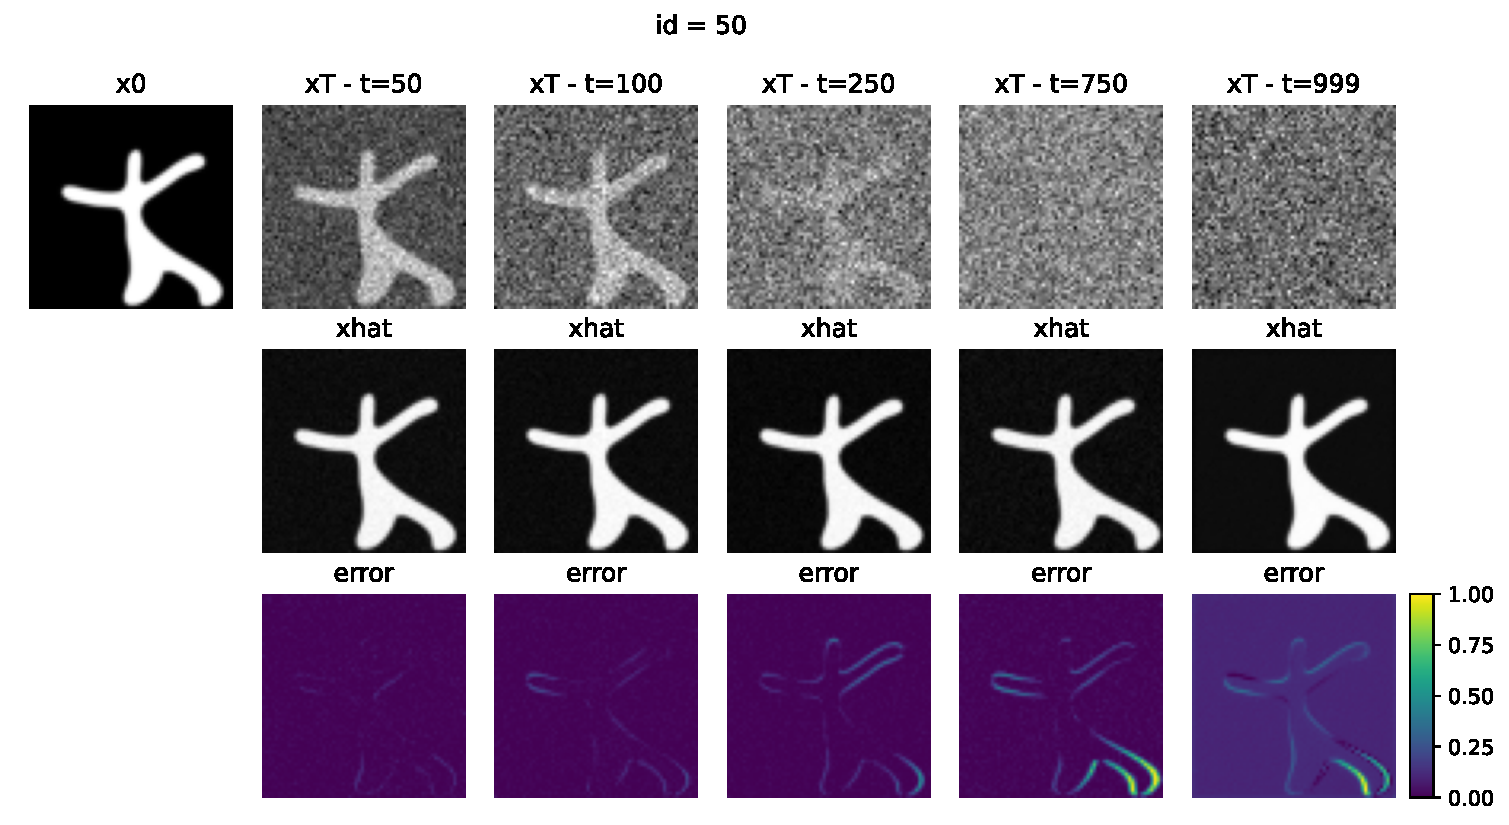
\includegraphics[width=0.75\linewidth]{figures/effect_noise_healthy.pdf}
    \caption{Effect of noise level on reconstructed images for healthy subject.}
    \label{fig:effect-noise-example-healthy}
\end{figure}

\begin{figure}[htbp]
  \centering
  \begin{subfigure}{0.75\linewidth}
    \includegraphics[width=\linewidth]{figures/effect_noise_darker_circle.pdf}
    \caption{Anomaly: \texttt{darker\_circle}}
  \end{subfigure}

  \begin{subfigure}{0.75\linewidth}
    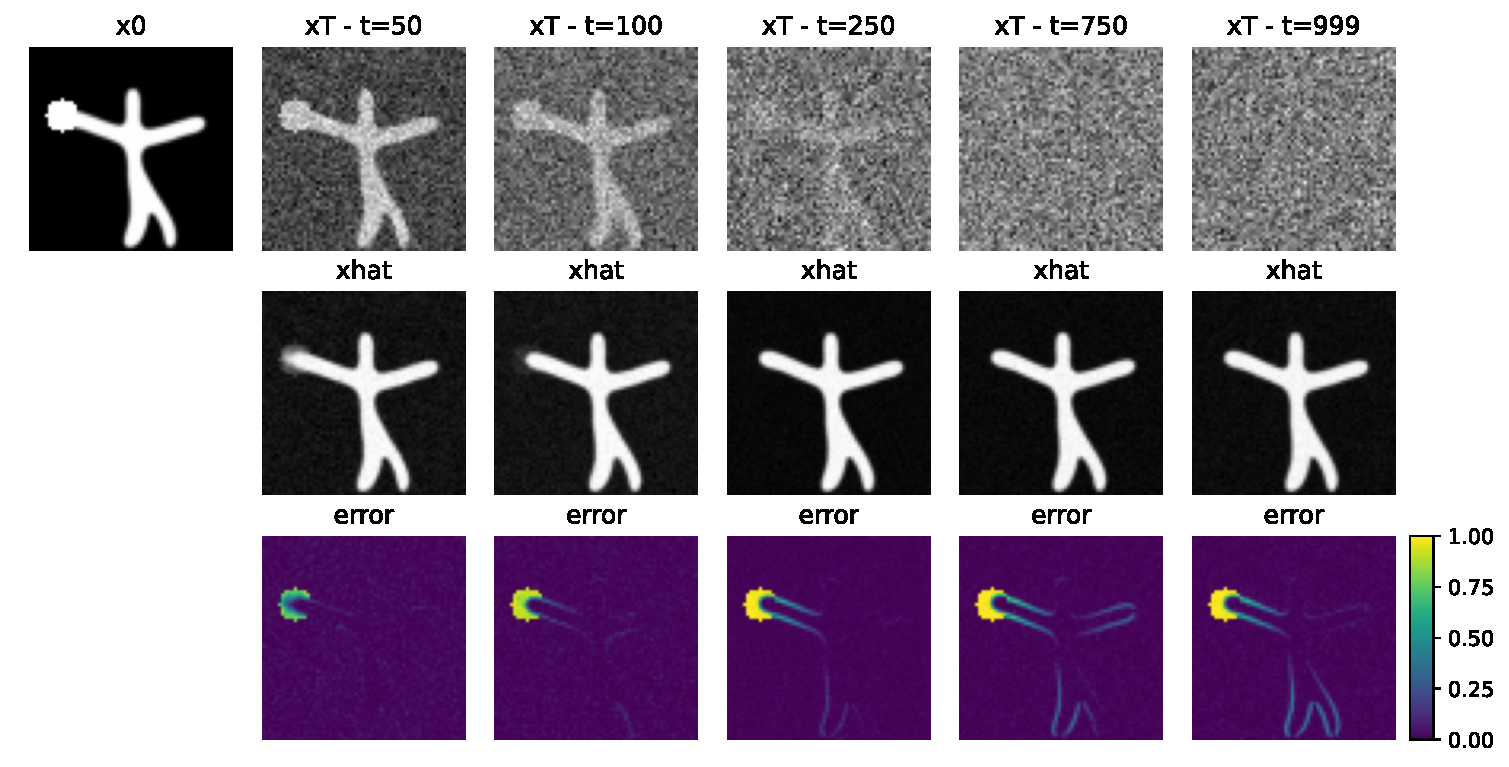
\includegraphics[width=\linewidth]{figures/effect_noise_growing_circle.pdf}
    \caption{Anomaly: \texttt{growing\_circle}}
  \end{subfigure}

  \caption{Effect of noise level on reconstructed images for anomalous subjects.}
  \label{fig:effect-noise-example-ano}
\end{figure}

\chapter{Feature Extractor Network}
\label{app:fe-layer}

\cref{fig:fe-layers} shows an example of feature maps from our feature extractor network $\text{FE} \Phi$. Each feature map is upscaled using linear interpolation to match the original spatial resolution of original image. The color displays the highest activation values across all channels at each pixel position, which is calculated as the mean of all channels. We observe that $\Phi$ effectively captures the perceptual structure of our figures at different scales. In particular, \texttt{stage2} focuses on overall shape of the \texttt{starman}, while \texttt{stage3} highlights the importance controlled points (head, legs and hands) of each figure. \texttt{stage4} operates at smallest resolution ($4, 4$), and due to the effect of upscaling, it does not capture any meaningful part of the original images that we can exploit. This is the reason why we utilize features from \{\texttt{stage2}, \texttt{stage3}\} to calculate our feature distances.

\begin{figure}[htbp]
  \centering
  \begin{subfigure}{0.75\linewidth}
    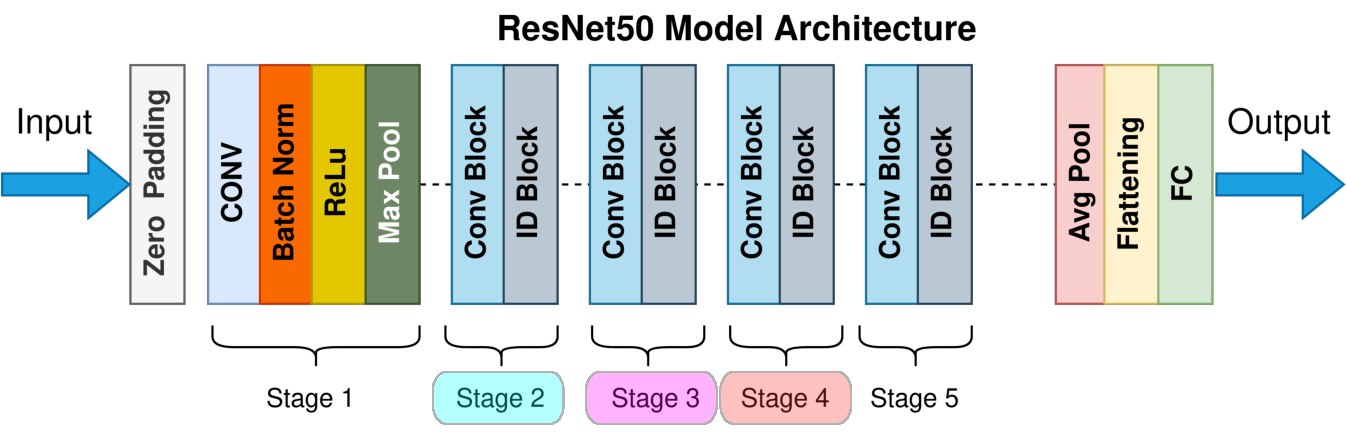
\includegraphics[width=\linewidth]{figures/resnet-50-arch.pdf}
    \caption{ResNet-50 architecture}
    \label{fig:resnet50-arch}
  \end{subfigure}

  \begin{subfigure}{0.75\linewidth}
    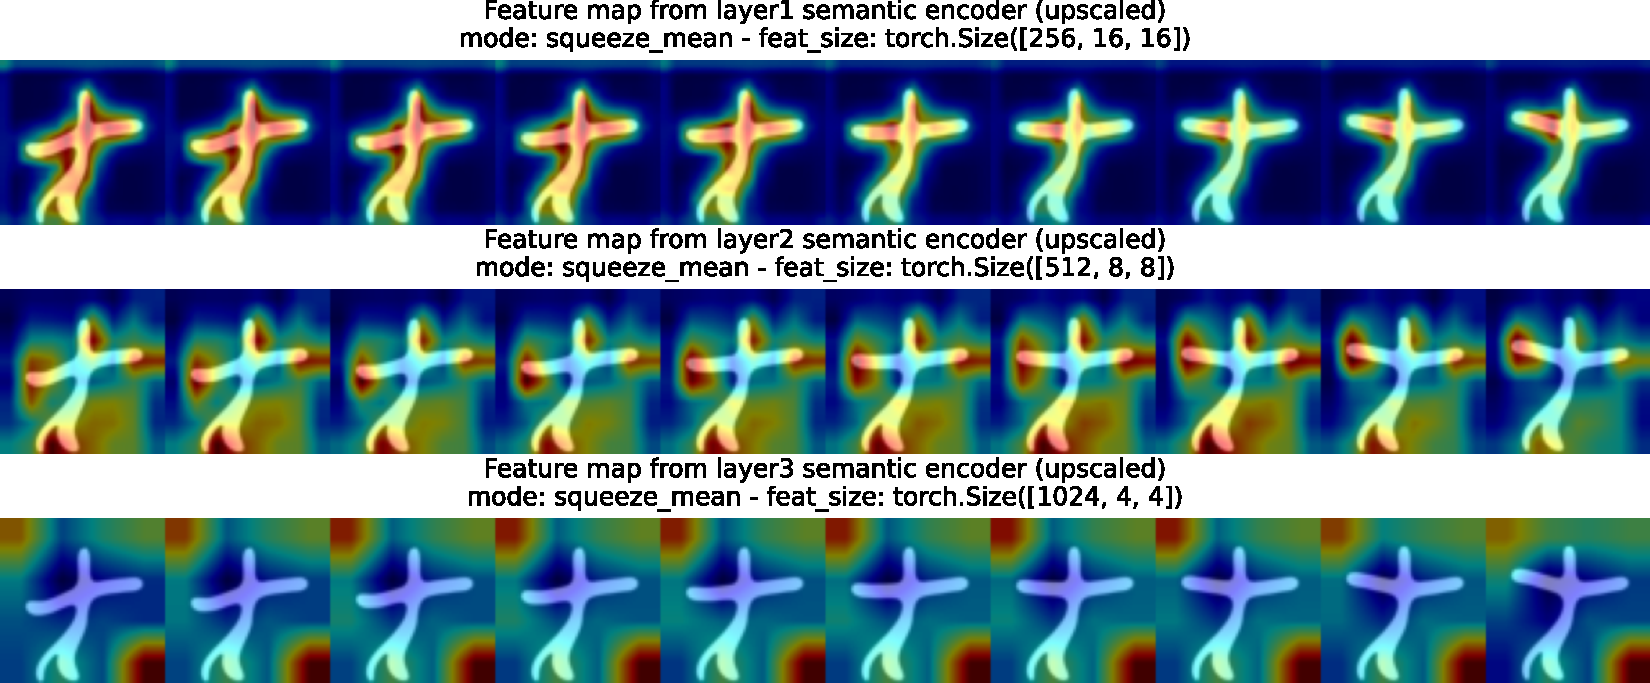
\includegraphics[width=\linewidth]{figures/fe-layer-healthy.pdf}
    \caption{Healthy subject}
    \label{fig:fe-layer-healthy}
  \end{subfigure}

  \begin{subfigure}{0.75\linewidth}
    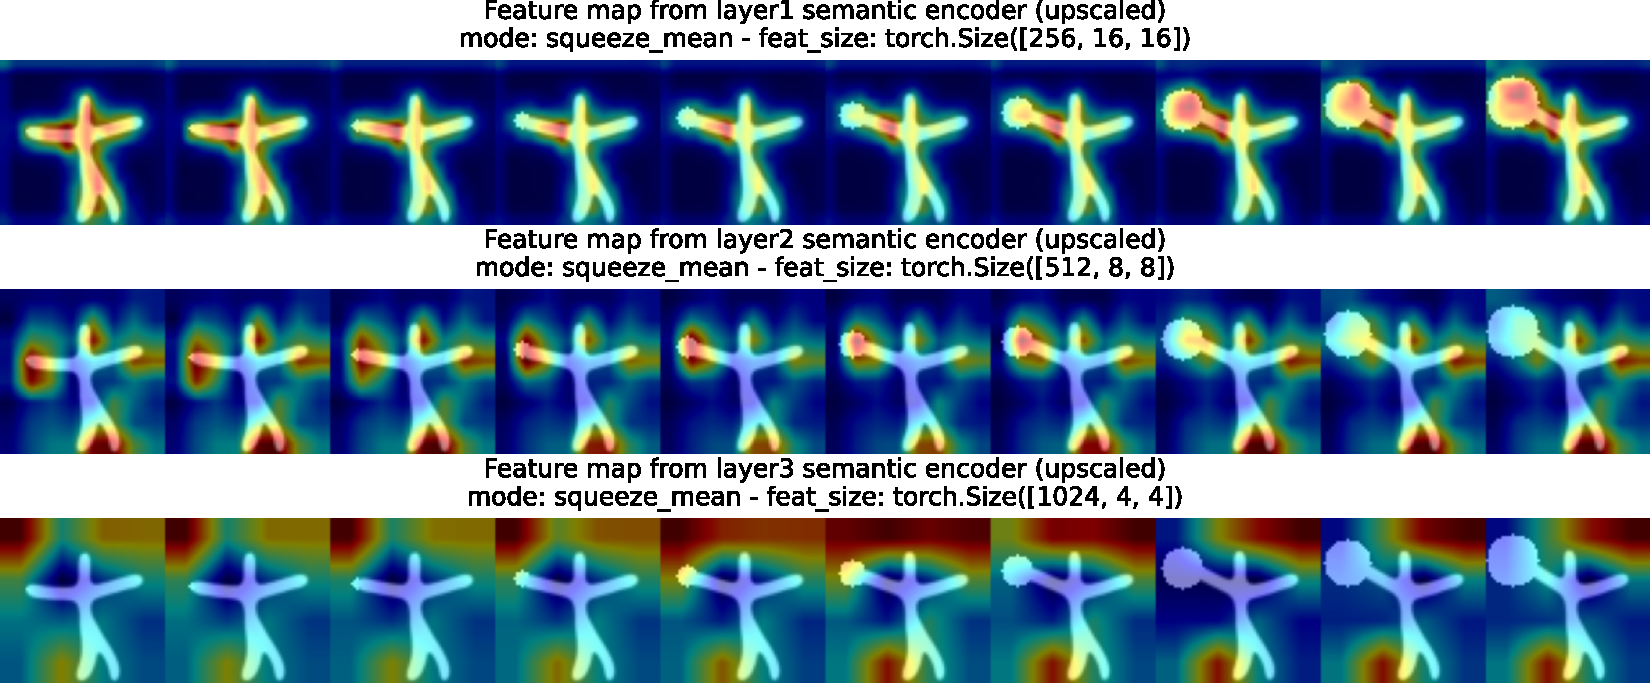
\includegraphics[width=\linewidth]{figures/fe-layer-anomaly.pdf}
    \caption{Anomaly subject}
    \label{fig:fe-layer-anomaly}
  \end{subfigure}
  \caption[Example feature maps from semantic encoder]{Example outputs from layers of Feature Extractor network $\Phi$ in \ac{SDM}. \cref{fig:resnet50-arch} shows ResNet-50 architecture. \cref{fig:fe-layer-healthy} and \cref{fig:fe-layer-anomaly} display example of outputs for healthy and anomalous subject, respectively. Notation: \texttt{stage2}, \texttt{stage3} and \texttt{stage4} from ResNet architecture correspond to \texttt{layer1}, \texttt{layer2} and \texttt{layer3} in our paper, respectively.}
  \label{fig:fe-layers}
\end{figure}

\chapter{Stochastic subcode manipulation}

We know that the stochastic subcode $\rvx_T^{\text{infer}}$ contains the fine-grained details about origin input, that the semantic encoder fails to capture. As shown in \cite{lozuponeLDAE2025,DiffAE}, this stochastic subcode, in combination with the semantic subcode from semantic encoder, is a powerful tool (latent variable) for us to manipulate the reconstructed images because they provide the best information of input. In this section, we show an example of utilizing this subcode to impute the missing images by interpolation. Given a starting time point $\mathbf{x}_{s}$ and ending time point $\mathbf{x}_{e}$, we can impute the missing images $\mathbf{x}_l$ at time point $s < l < e$ by interpolating both semantic subcode and stochastic subcode. From the two input time points, we can extract their semantic and stochastic representation $(\mathbf{y}_{\text{sem}}^s, \mathbf{y}_{\text{sem}}^e)$ and $(\mathbf{x}_{\text{infer}}^s, \mathbf{x}_{\text{infer}}^e)$, respectively. Based on these spaces, the intermediate semantic and stochastic subcode of $\mathbf{x}_l$ can be formulated using two methods, following \cite{lozuponeLDAE2025}:

\paragraph{\texttt{lerp-slerp} interpolation}: we perform linear interpolation in semantic space and spherical interpolation in stochastic one:

\begin{align*}
  \mathrm{LERP}(\mathbf{y}_{\text{sem}}^s, \mathbf{y}_{\text{sem}}^e; \alpha) &= (1 - \alpha) \mathbf{y}_{\text{sem}}^s + \alpha \mathbf{y}_{\text{sem}}^e \\
  \mathrm{SLERP}(\mathbf{x}_{\text{infer}}^s, \mathbf{x}_{\text{infer}}^e; \alpha) &=
  \frac{\sin((1 - \alpha)\theta)}{\sin(\theta)} \mathbf{x}_{\text{infer}}^s +
  \frac{\sin(\alpha \theta)}{\sin(\theta)} \mathbf{x}_{\text{infer}}^e
\end{align*}

where the angle $\theta$ between $\langle \mathbf{x}_{\text{infer}}^s, \mathbf{x}_{\text{infer}}^e \rangle$ is calculated as: 
\begin{align*}
    \theta = \arccos \left( \frac{\langle \mathbf{x}_{\text{infer}}^s, \mathbf{x}_{\text{infer}}^e \rangle}{\| \mathbf{x}_{\text{infer}}^s \| \cdot \| \mathbf{x}_{\text{infer}}^e \|} \right)
\end{align*}

Coefficient $\alpha$ is the offset of target time point $l$ with respect to the starting and ending time points, and is defined as $\alpha = \frac{l - s}{e - s}$. We note that $\alpha \in [0, 1]$. Subsequently, $\mathbf{x}_l$ is imputed as reconstruction (decode) image by using $(\mathbf{y}_{\text{sem}}^l, \mathbf{x}_{\text{infer}}^l)$

\paragraph{\texttt{lerp-lerp} interpolation}: we perform linear interpolation in both semantic and stochastic space, using the same above formulas. 

\cref{fig:interpolation-healthy} and \cref{fig:interpolation-ano} show quantitative examples of interpolation using both methods, for both healthy and anomalous subjects. 

\begin{figure}[htbp]
  \centering
  \begin{subfigure}{0.8\linewidth}
    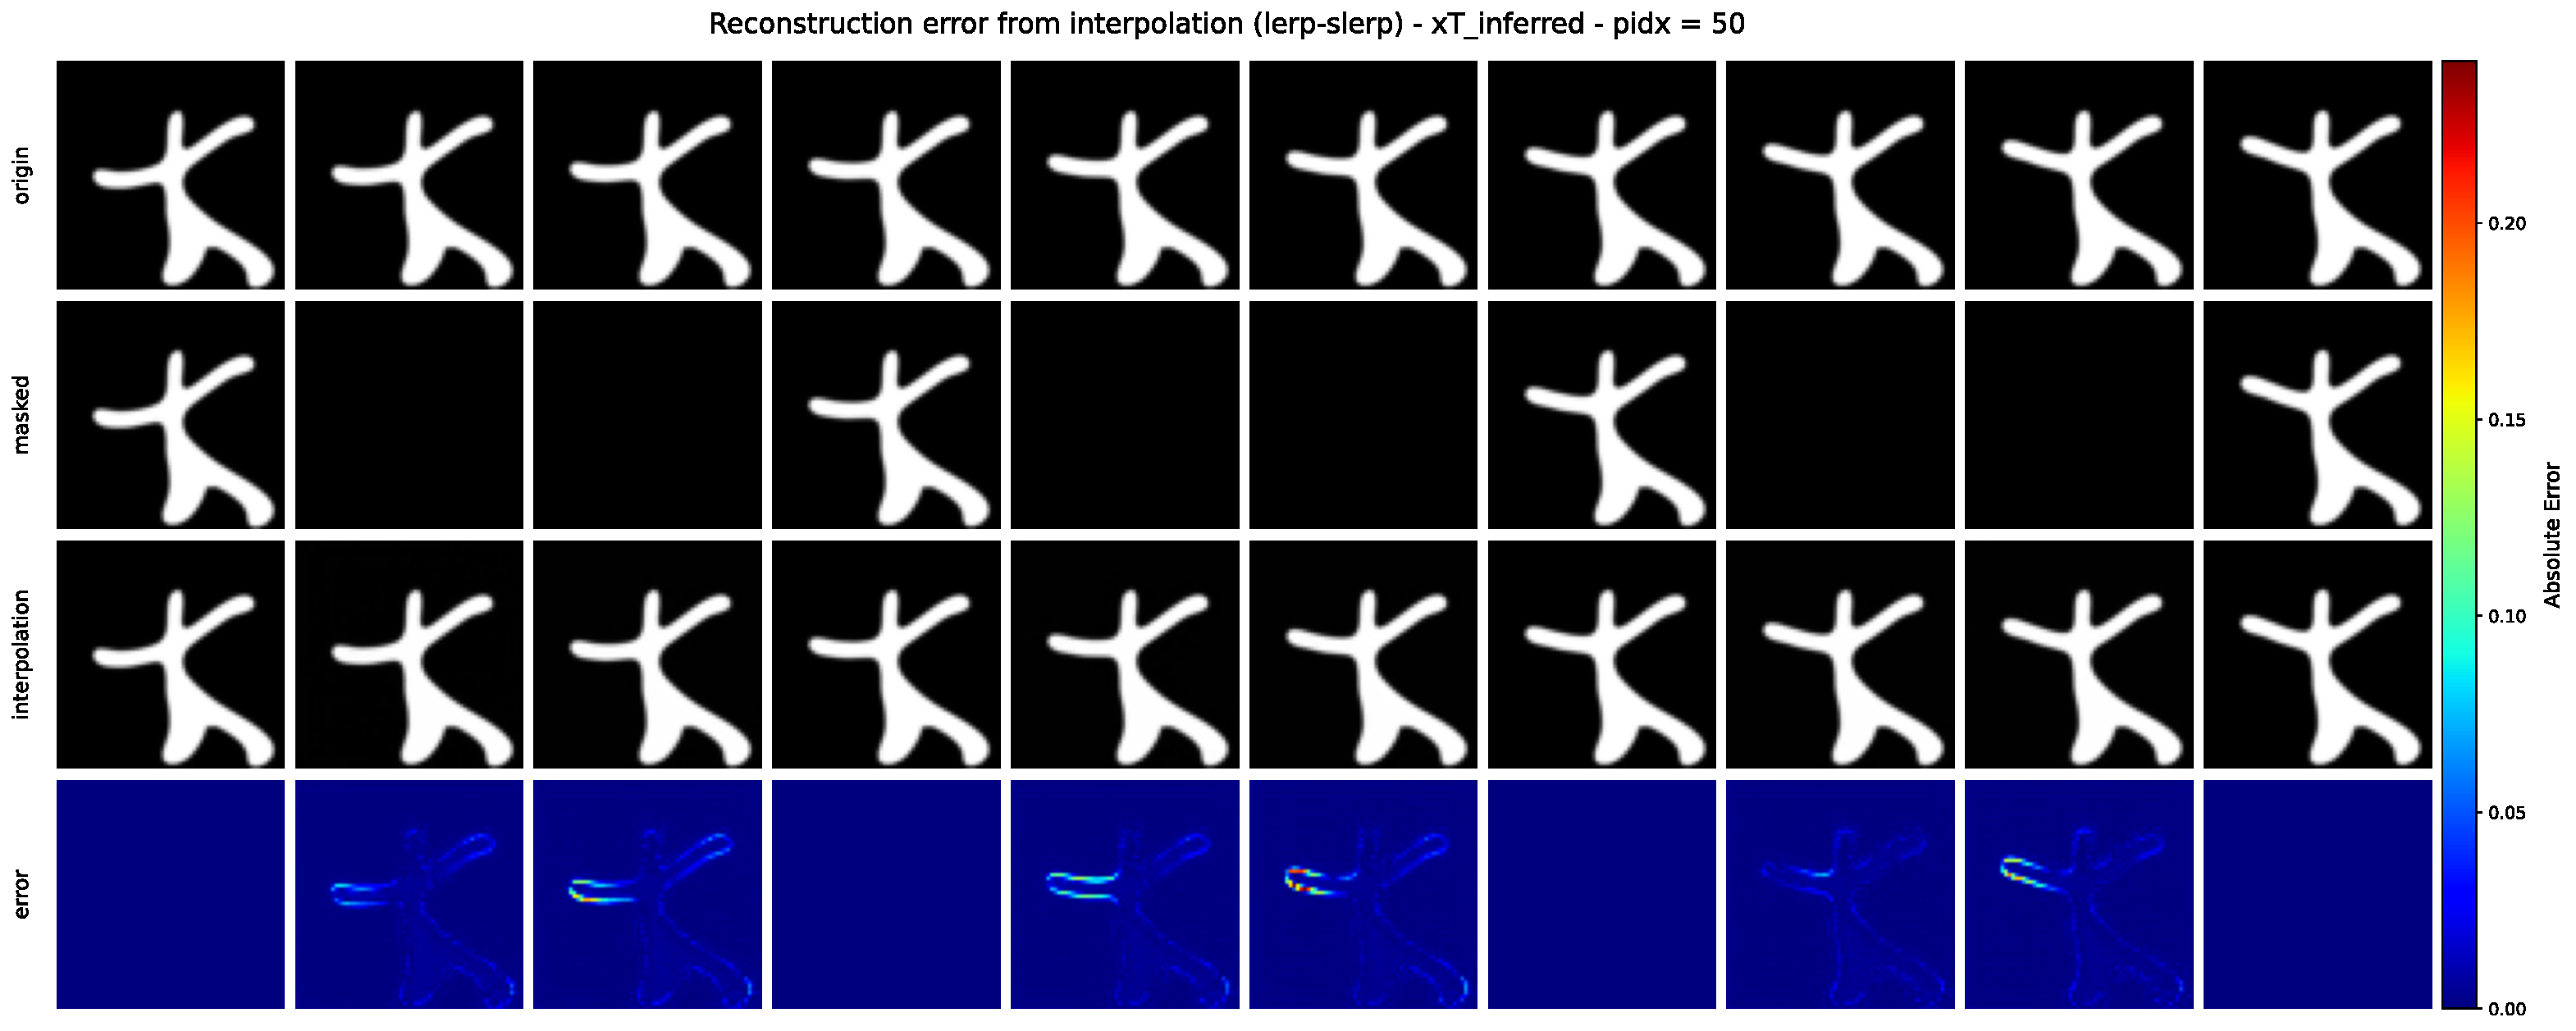
\includegraphics[width=\linewidth]{figures/interpolation-lerp-lerp-id-50.pdf}
    \caption{\texttt{lerp-lerp} interpolation}
  \end{subfigure}

  \begin{subfigure}{0.8\linewidth}
    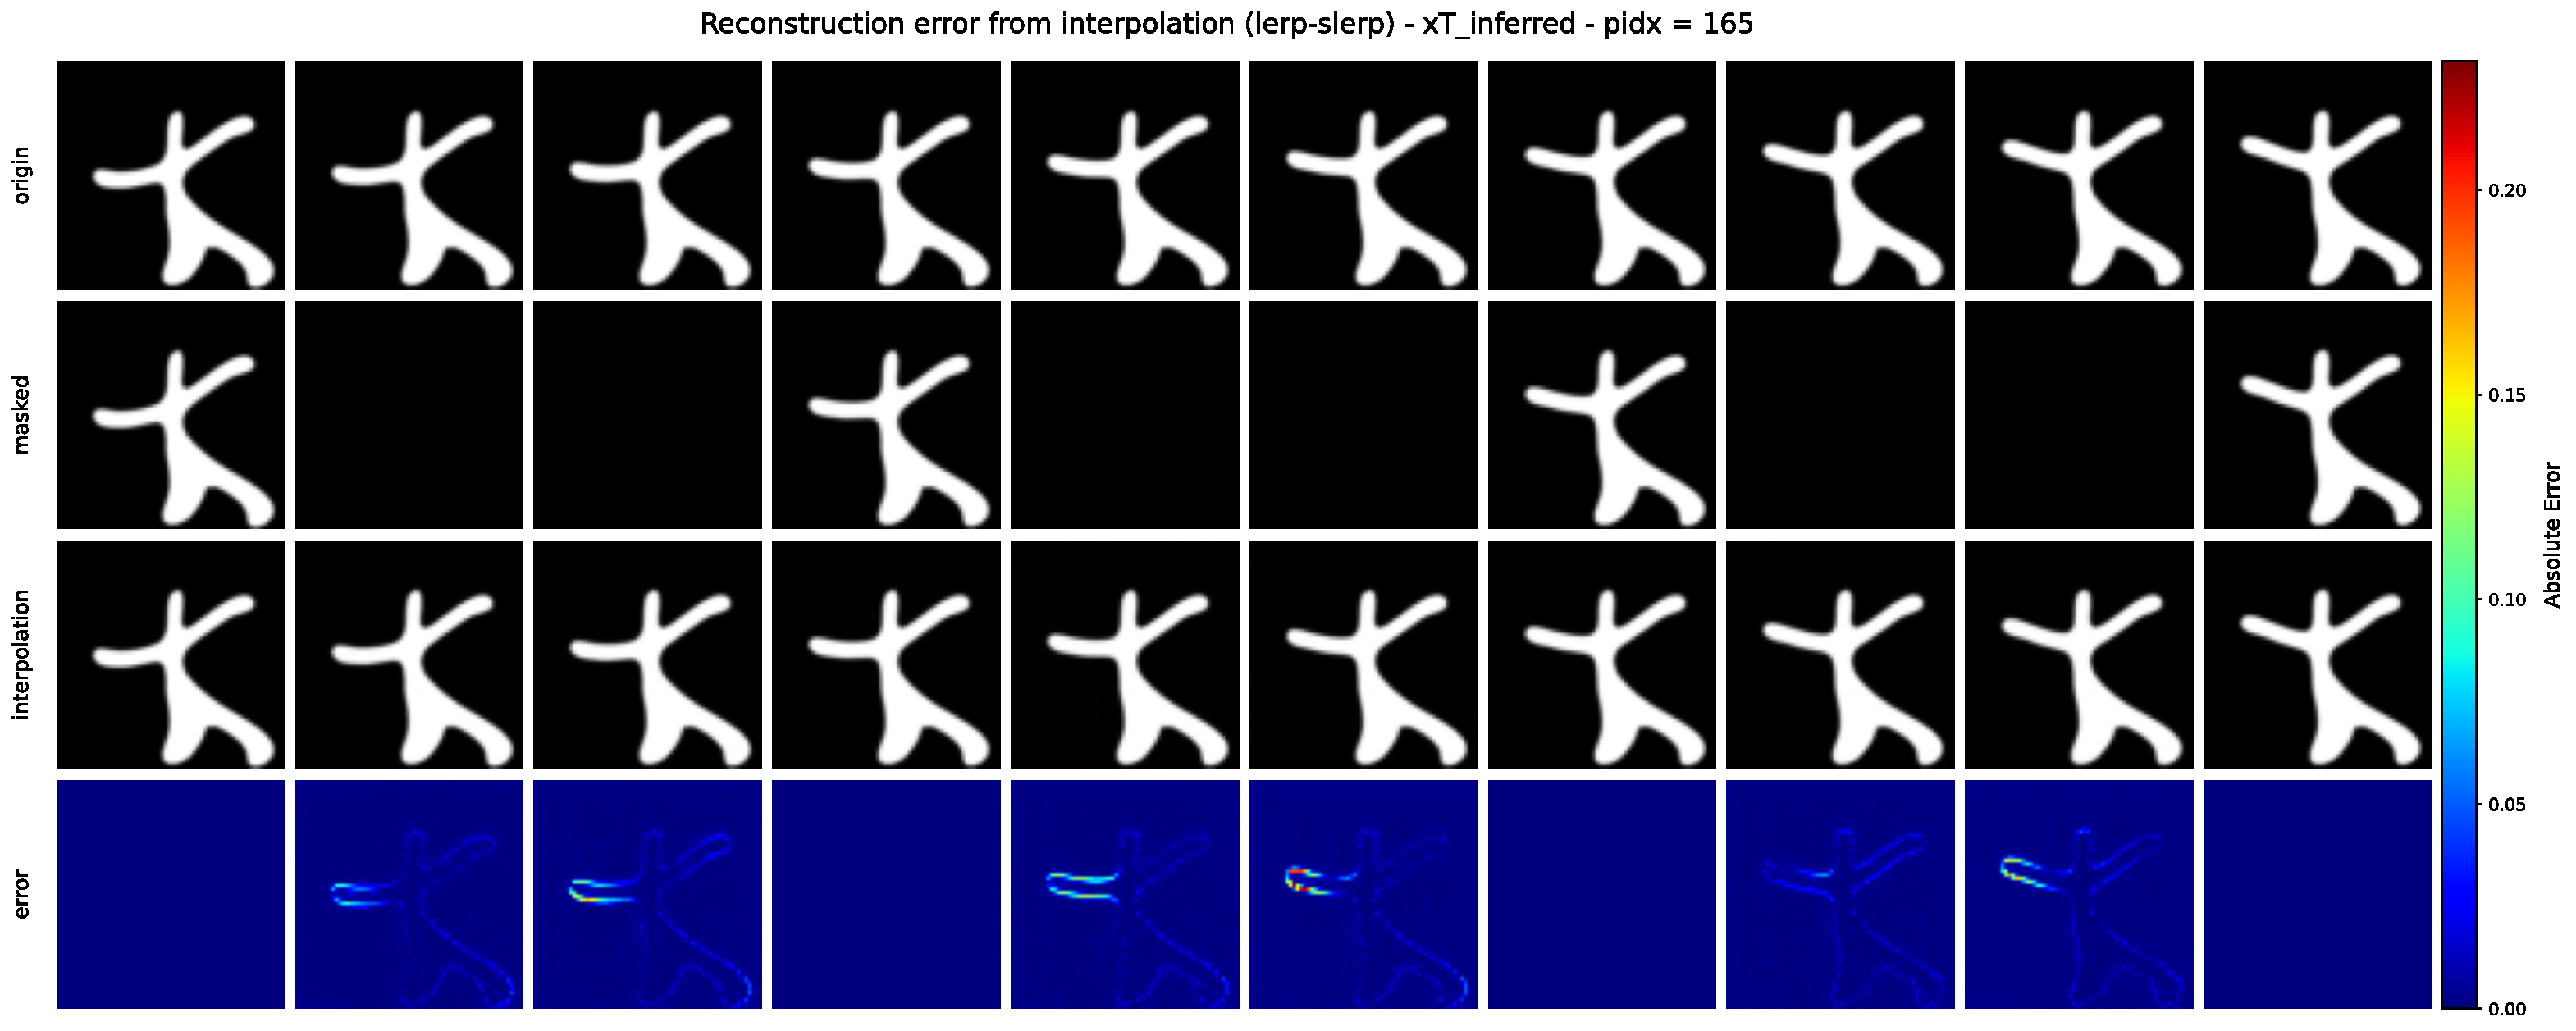
\includegraphics[width=\linewidth]{figures/interpolation-lerp-slerp-id-50.pdf}
    \caption{\texttt{lerp-slerp} interpolation}
  \end{subfigure}
  \caption{Interpolation from stochastic subcode for healthy subject. }
  \label{fig:interpolation-healthy}
\end{figure}

\begin{figure}[htbp]
  \centering
  \begin{subfigure}{0.8\linewidth}
    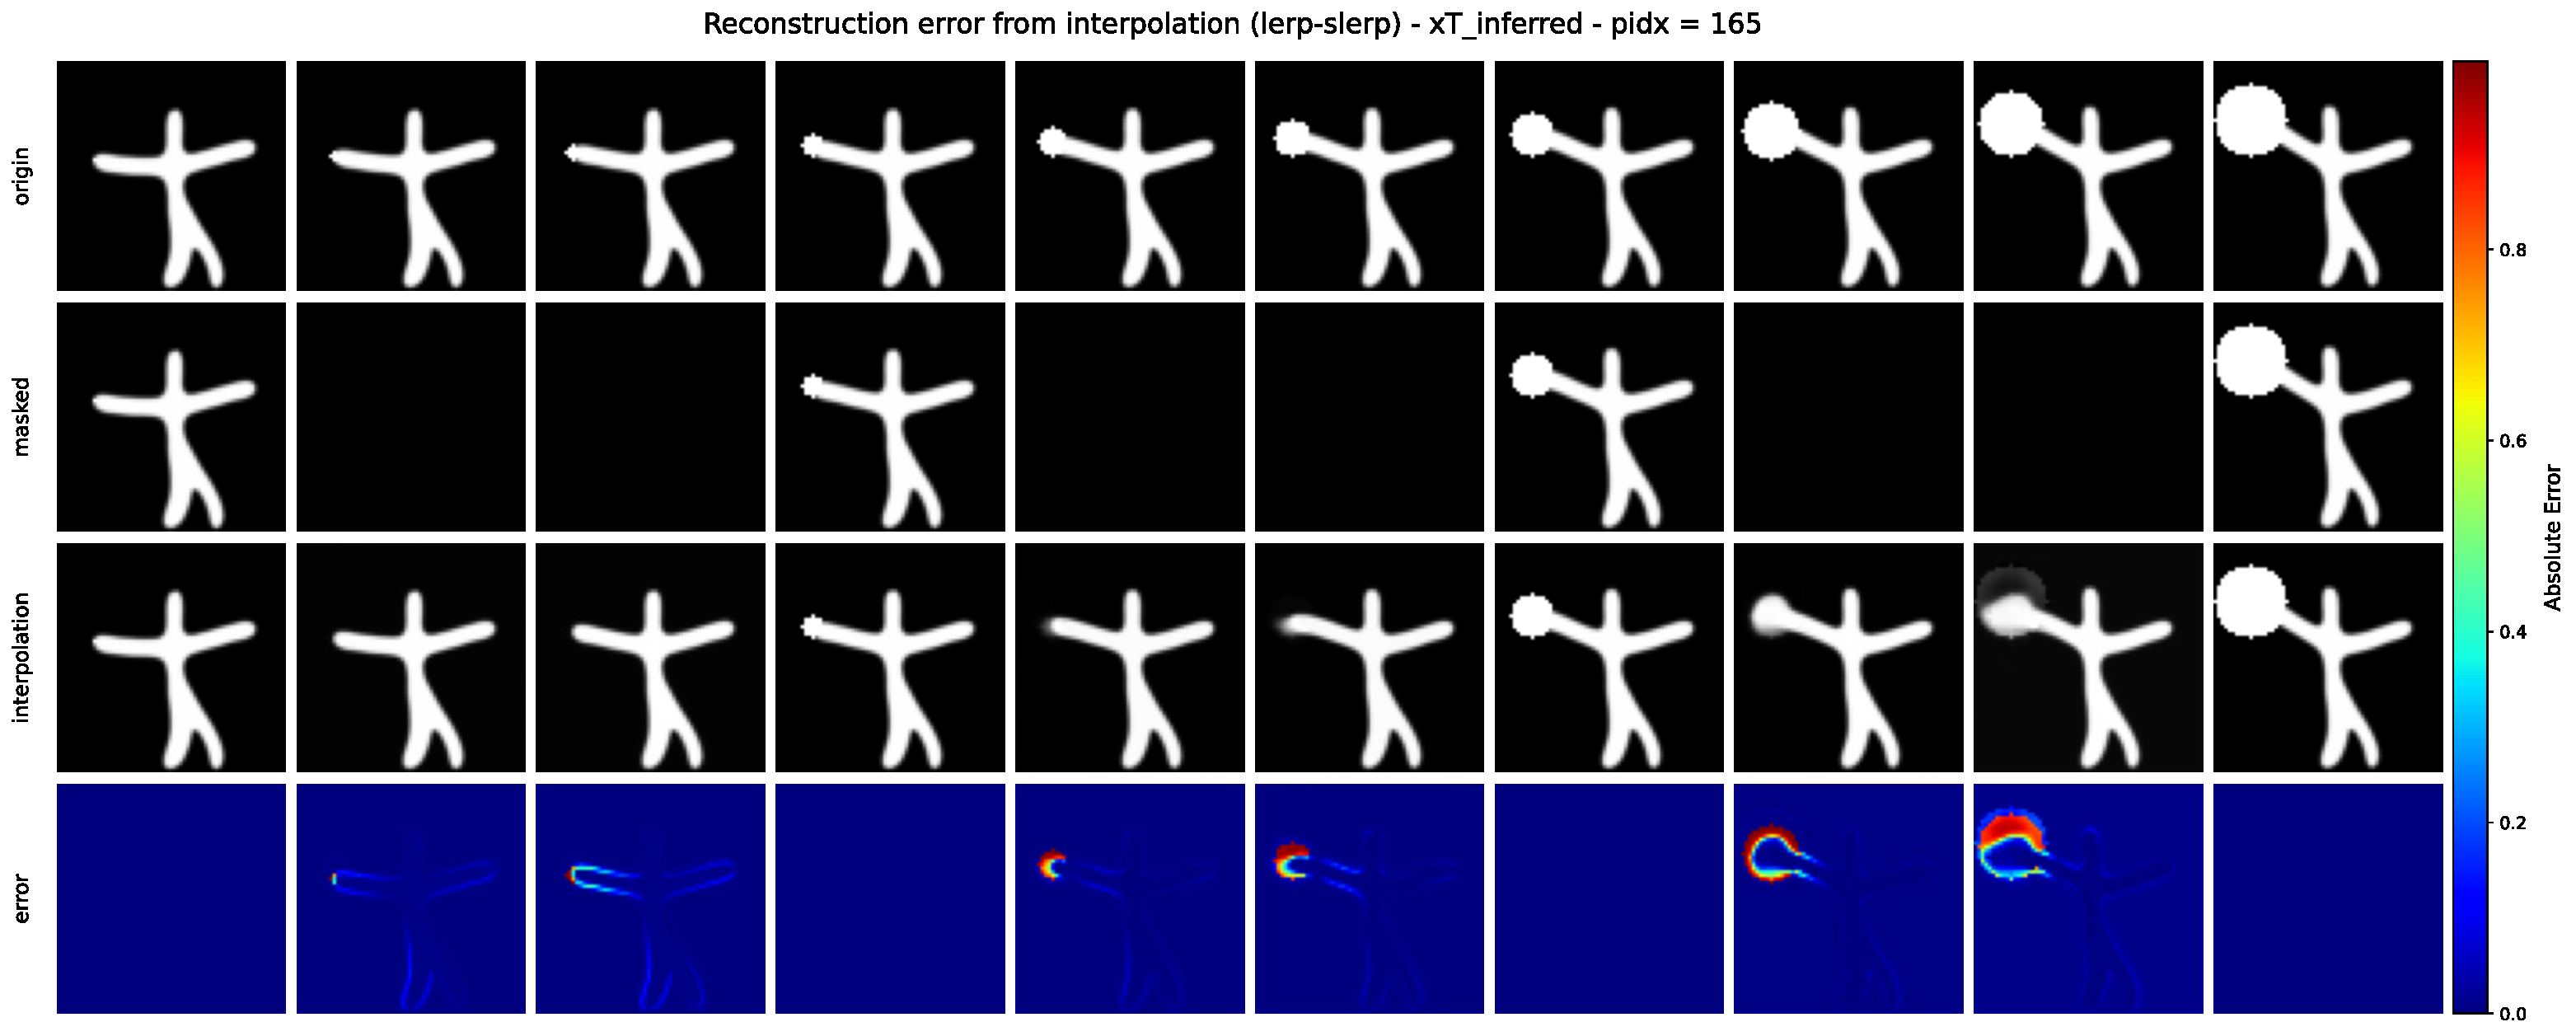
\includegraphics[width=\linewidth]{figures/interpolation-lerp-lerp-id-165.pdf}
    \caption{\texttt{lerp-lerp} interpolation}
  \end{subfigure}

  \begin{subfigure}{0.8\linewidth}
    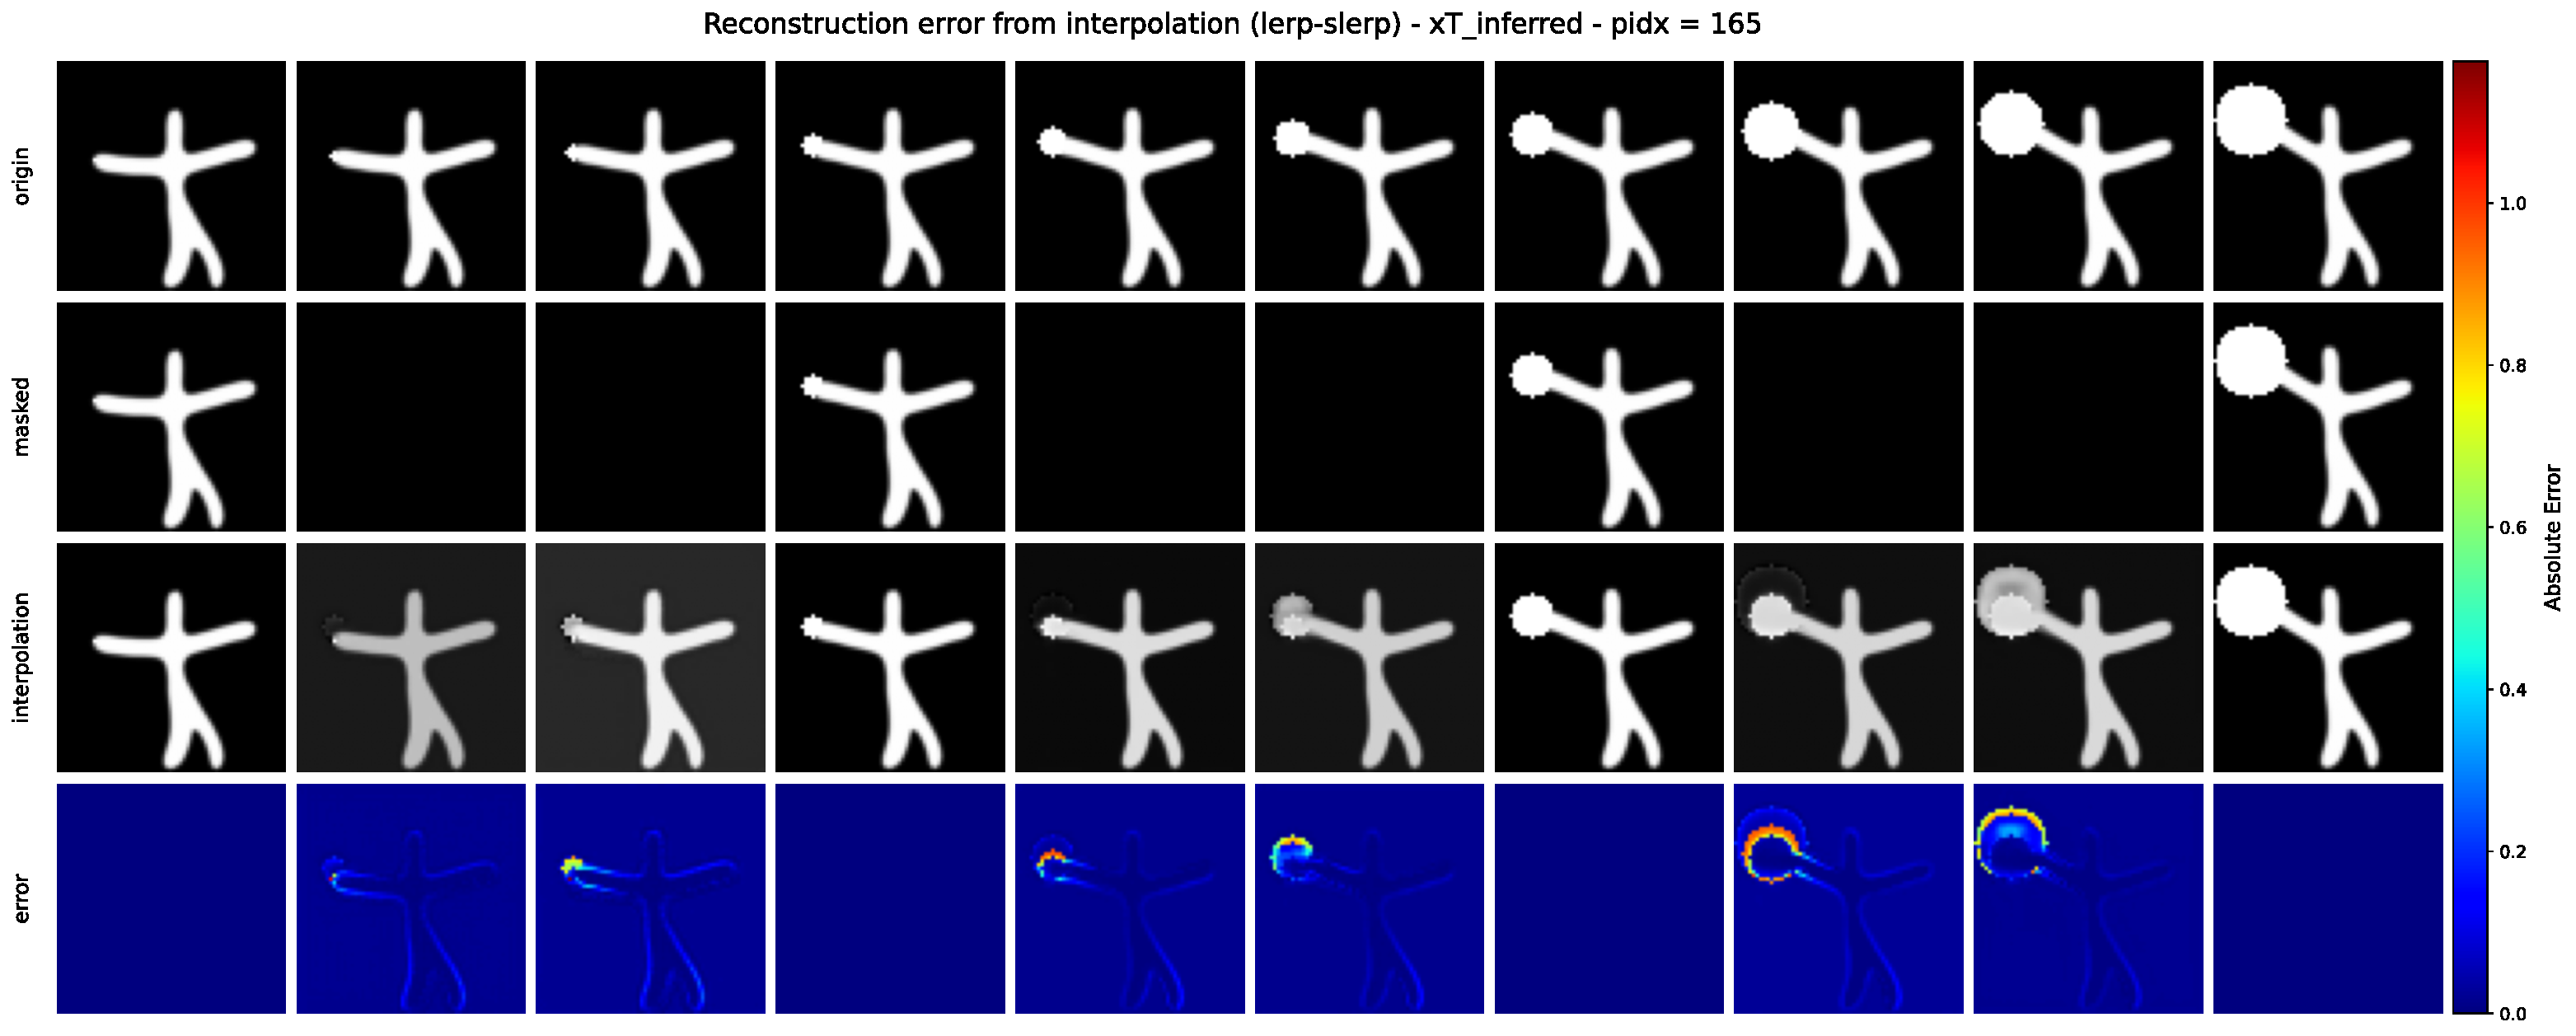
\includegraphics[width=\linewidth]{figures/interpolation-lerp-slerp-id-165.pdf}
    \caption{\texttt{lerp-slerp} interpolation}
  \end{subfigure}
  \caption{Interpolation from stochastic subcode for healthy subject. }
  \label{fig:interpolation-ano}
\end{figure}

% \clearpage
\chapter{More examples of LAFM Anomaly score maps}
\begin{figure}[htbp]
  \centering
  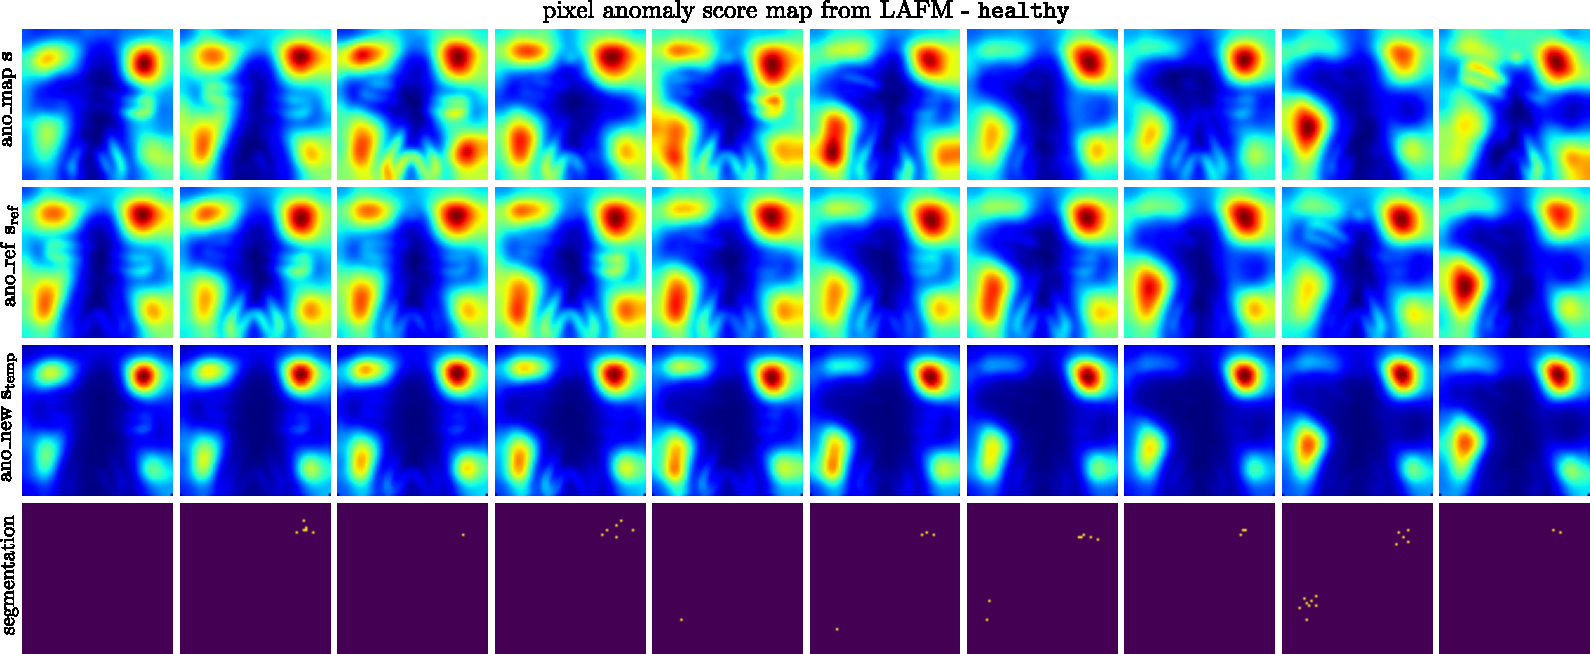
\includegraphics[width=0.75\linewidth]{figures/app-lafm-healthy.pdf}
  \caption[Example: anomaly segmentation from LAFM - \texttt{healthy} subject]{Example of anomaly score map from LAFM for healthy subject. From top to bottom: input score map (from FAM), anomaly map references, updated score map (LAFM), anomaly segmentation (Yen threshold).}
\end{figure}

\begin{figure}[htbp]
  \centering
  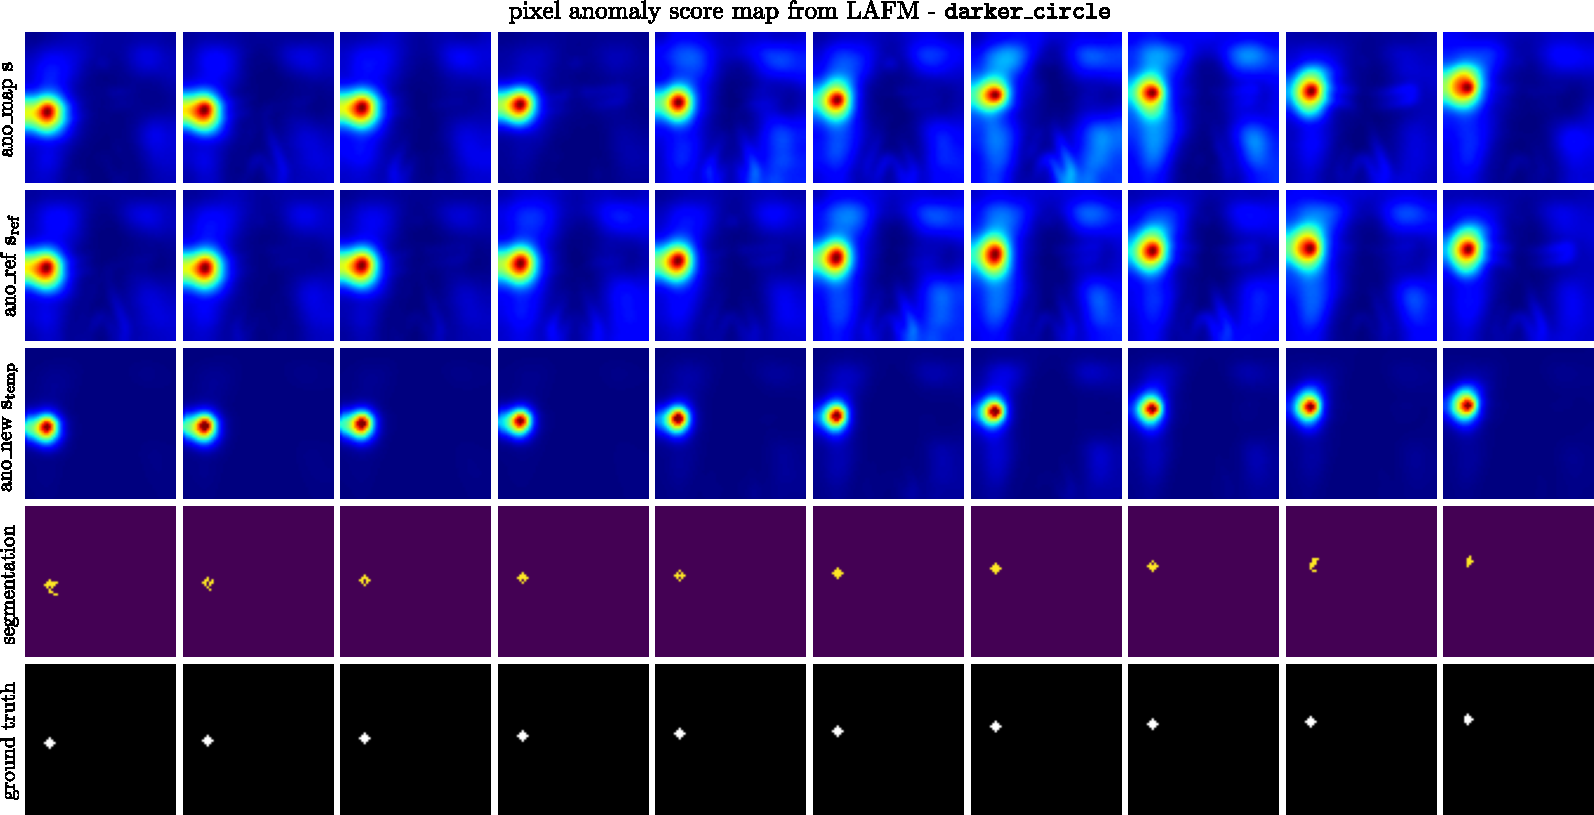
\includegraphics[width=0.75\linewidth]{figures/app-lafm-darkercircle.pdf}
  \caption[Example: anomaly segmentation from LAFM - \texttt{darker\_circle}]{Example of anomaly score map from LAFM for anomaly \texttt{darker\_circle} subject. From top to bottom: input score map (from FAM), anomaly map references, updated score map (LAFM), anomaly segmentation (Yen threshold) and ground truth annotation.}
\end{figure}

\begin{figure}[htbp]
  \centering
  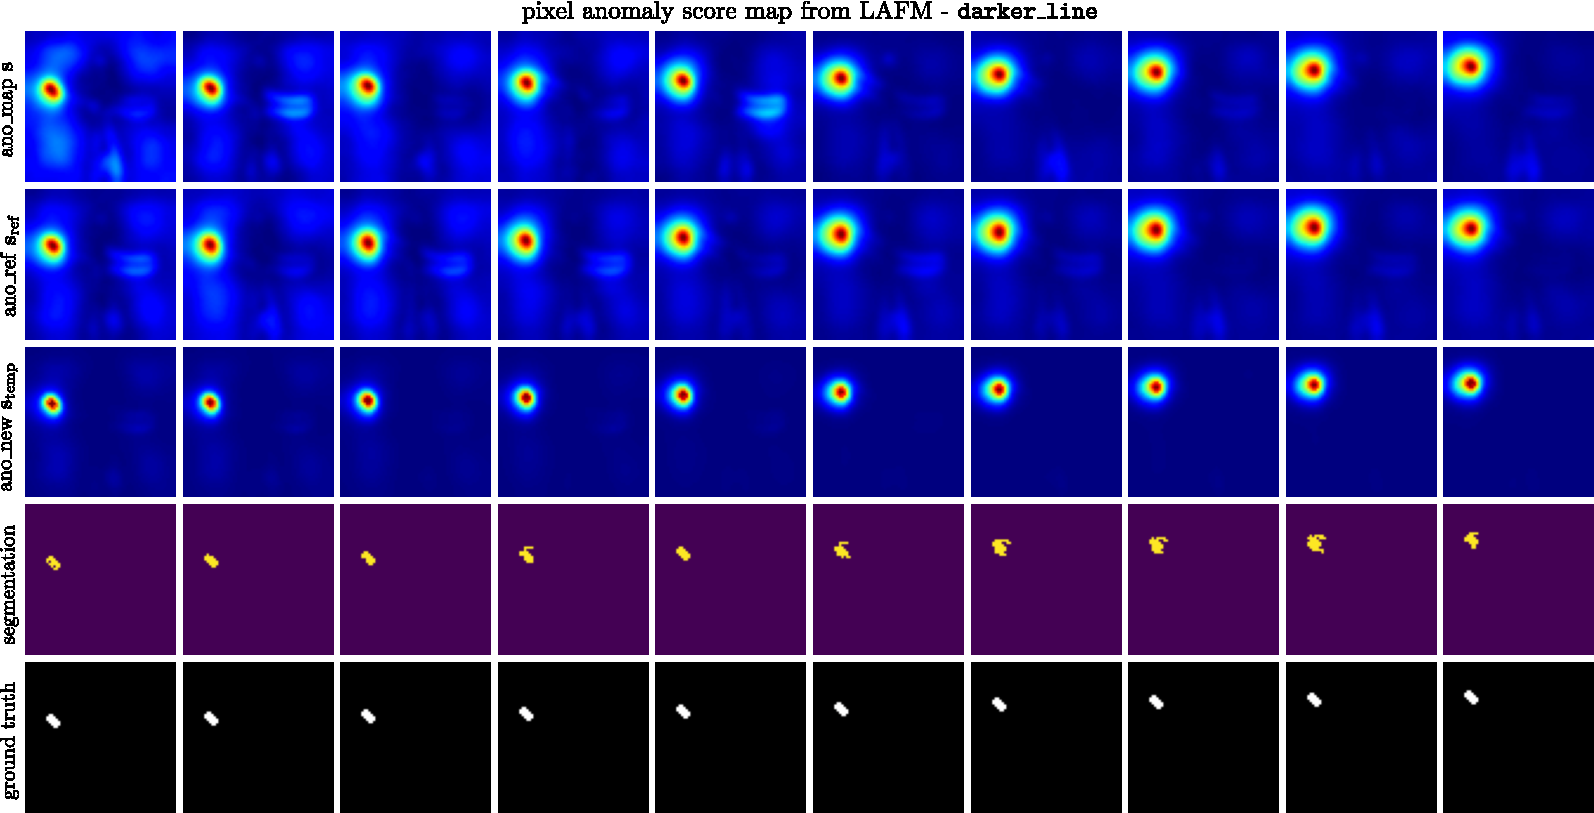
\includegraphics[width=0.75\linewidth]{figures/app-lafm-darkerline.pdf}
  \caption[Example: anomaly segmentation from LAFM - \texttt{darker\_line}]{Example of anomaly score map from LAFM for anomaly \texttt{darker\_line} subject. From top to bottom: input score map (from FAM), anomaly map references, updated score map (LAFM), anomaly segmentation (Yen threshold) and ground truth annotation.}
\end{figure}
\FloatBarrier


\end{document}